% ---------------------------------------------------------------------------------
% Main tex file
% $Id: Thesis.tex,v 1.55 2012/07/23 16:36:02 matsch Exp $

\documentclass[
twoside=true,
headsepline,     % Line under page header
headings=normal,
open=right,
numbers=noenddot, % Otherwise there will be a dot after the chapter numbering in case letters are used somewhere e.g. in the appendix
a4paper
]{scrreprt} %report scrreprt
\addtolength{\topmargin}{-0.2cm}
\setlength{\textwidth}{15cm}
\setlength{\textheight}{22.4cm}
\setlength{\oddsidemargin}{0cm}
\setlength{\evensidemargin}{0.85cm} 

\usepackage[automark,headsepline]{scrpage2}
\pagestyle{scrheadings}
\clearscrheadfoot
\ihead{\headmark}
\ohead{\pagemark}
\cfoot{}
\setcounter{secnumdepth}{3}
\setcounter{tocdepth}{3}

% Alter some LaTeX defaults for better treatment of figures,
% from http://mintaka.sdsu.edu/GF/bibliog/latex/floats.html
% See p.105 of "TeX Unbound" for suggested values.
% See pp. 199-200 of Lamport's "LaTeX" book for details.
% General parameters, for ALL pages:
\renewcommand{\topfraction}{0.9}	% max fraction of floats at top
\renewcommand{\bottomfraction}{0.8}	% max fraction of floats at bottom
% Parameters for TEXT pages (not float pages):
%\setcounter{topnumber}{2}
%\setcounter{bottomnumber}{2}
%\setcounter{totalnumber}{4}     % 2 may work better
%\setcounter{dbltopnumber}{2}    % for 2-column pages
\renewcommand{\dbltopfraction}{0.9}	% fit big float above 2-col. text
\renewcommand{\textfraction}{0.07}	% allow minimal text w. figs
% Parameters for FLOAT pages (not text pages):
\renewcommand{\floatpagefraction}{0.7}	% require fuller float pages
% N.B.: floatpagefraction MUST be less than topfraction !!
\renewcommand{\dblfloatpagefraction}{0.7}	% require fuller float pages
% remember to use [htp] or [htpb] for placement



\usepackage{amsfonts}
\usepackage{amsmath}  % Correct size switching in mathmode when using \text{} instead of \textrm{}
\usepackage{amssymb} 
\usepackage{amstext} 
\usepackage{cite}
\usepackage{graphicx}
\usepackage{booktabs}
\usepackage{tabularx}
\usepackage{multirow}
\usepackage{setspace}
\usepackage{rotating}
\usepackage{float}
\usepackage{afterpage}
\usepackage{verbatim}
% \usepackage{ptdr-definitions}

%\usepackage{setspace}
%\doublespacing

\hyphenation{Super-sym-me-try}
\hyphenation{maximum-like-li-hood}

% ---------------------------------------------------------------------------------
% Collection of user-defined commands
% $Id: definitions.tex,v 1.46 2012/07/23 16:36:01 matsch Exp $

\usepackage{amsmath}
\usepackage{xspace}

\newcommand{\figmultican}[1]{
  \centering
  \includegraphics[width=0.85\textwidth]{figures/#1}
}
\newcommand{\figone}[1]{
  \centering
  \includegraphics[width=0.49\textwidth]{figures/#1}
}
\newcommand{\figtwo}[2]{
  \centering
  \begin{tabular}{@{}c@{}p{0.02\textwidth}@{}c@{}}
    \includegraphics[width=0.49\textwidth]{figures/#1} & &
    \includegraphics[width=0.49\textwidth]{figures/#2} \\
  \end{tabular}
}
\newcommand{\figthree}[3]{
  \centering
  \begin{tabular}{@{}c@{}p{0.02\textwidth}@{}c@{}}
    \includegraphics[width=0.49\textwidth]{figures/#1} & &
    \includegraphics[width=0.49\textwidth]{figures/#2} \\
    \includegraphics[width=0.49\textwidth]{figures/#3} & & \\
  \end{tabular}
}
\newcommand{\figfour}[4]{
  \centering
  \begin{tabular}{@{}c@{}p{0.02\textwidth}@{}c@{}}
    \includegraphics[width=0.49\textwidth]{figures/#1} & &
    \includegraphics[width=0.49\textwidth]{figures/#2} \\
    \includegraphics[width=0.49\textwidth]{figures/#3} & &
    \includegraphics[width=0.49\textwidth]{figures/#4} \\
  \end{tabular}
}
\newcommand{\figfive}[5]{
  \centering
  \begin{tabular}{@{}c@{}p{0.2\textwidth}@{}c@{}}
    \includegraphics[width=0.4\textwidth]{figures/#1} & &
    \includegraphics[width=0.4\textwidth]{figures/#2} \\
    \includegraphics[width=0.4\textwidth]{figures/#3} & &
    \includegraphics[width=0.4\textwidth]{figures/#4} \\
    \includegraphics[width=0.4\textwidth]{figures/#5} & & \\
  \end{tabular}
}
\newcommand{\figsix}[6]{
  \centering
  \begin{tabular}{@{}c@{}p{0.1\textwidth}@{}c@{}}
    \includegraphics[width=0.4\textwidth]{figures/#1} & &
    \includegraphics[width=0.4\textwidth]{figures/#2} \\
    \includegraphics[width=0.4\textwidth]{figures/#3} & &
    \includegraphics[width=0.4\textwidth]{figures/#4} \\
    \includegraphics[width=0.4\textwidth]{figures/#5} & &
    \includegraphics[width=0.4\textwidth]{figures/#6}  \\
  \end{tabular}
}


\newcommand{\emptybox}[1]{\parbox[c][#1]{0pt}{}}

%\newcommand{\tobechecked}{\textcolor{red}{\textbf{(to be checked)}}}
%\newcommand{\alreadydefined}[1]{\textcolor{red}{\textbf{(#1 already defined?)}}}
%\newcommand{\todo}[1]{\textcolor{blue}{{\textbf{TODO: }\textit{#1}}}}
%\newcommand{\fixme}[1]{\textcolor{red}{{\textbf{FIXME: }\textit{#1}}}}
%\newcommand{\addref}{\textcolor{blue}{ADD REFERENCE}}
%\newcommand{\addfig}[1]{\textcolor{red}{\textbf{ADD FIGURE: }\textit{#1}}}

% Sectioning
\newcommand{\qsec}[1]{Section~\ref{#1}}
\newcommand{\qsecs}[2]{Sections~\ref{#1} and~\ref{#2}}
\newcommand{\qsectosec}[2]{Sections~\ref{#1} to~\ref{#2}}
\newcommand{\cfqsec}[1]{cf.\ Section~\ref{#1}}
\newcommand{\figs}{Figs.}
\newcommand{\qfig}[1]{Fig.~\ref{#1}}
\newcommand{\qfigs}[2]{Figs.~\ref{#1} and~\ref{#2}}
\newcommand{\qfigtofig}[2]{Figs.~\ref{#1} to~\ref{#2}}
\newcommand{\cfqfig}[1]{cf.\ Fig.~\ref{#1}}
\newcommand{\qsubfig}[2]{Fig.~\ref{#1}~(\textit{#2})}
\newcommand{\qtab}[1]{Table~\ref{#1}}
\newcommand{\qtabs}[2]{Tables~\ref{#1} and~\ref{#2}}
\newcommand{\qtabtotab}[2]{Tables~\ref{#1} to~\ref{#2}}
\newcommand{\cfqtab}[1]{cf.\ Table~\ref{#1}}
\newcommand{\qeq}[1]{Eq.~\eqref{#1}}

% Units
\newcommand{\tev}{\ensuremath{\,\text{Te}\kern-0.06667em\text{V}}\xspace}
\newcommand{\gev}{\ensuremath{\,\text{Ge}\kern-0.06667em\text{V}}\xspace}
\newcommand{\mev}{\ensuremath{\,\text{Me}\kern-0.06667em\text{V}}\xspace}
\newcommand{\kev}{\ensuremath{\,\text{ke}\kern-0.06667em\text{V}}\xspace}
\newcommand{\ev}{\ensuremath{\,\text{e}\kern-0.06667em\text{V}}\xspace}
\newcommand{\tevnospace}{\ensuremath{\text{Te}\kern-0.06667em\text{V}}\xspace}
\newcommand{\gevnospace}{\ensuremath{\text{Ge}\kern-0.06667em\text{V}}\xspace}
\newcommand{\mevnospace}{\ensuremath{\text{Me}\kern-0.06667em\text{V}}\xspace}
\newcommand{\kevnospace}{\ensuremath{\text{ke}\kern-0.06667em\text{V}}\xspace}
\newcommand{\evnospace}{\ensuremath{\text{e}\kern-0.06667em\text{V}}\xspace}
\newcommand{\km}{\ensuremath{\,\text{km}}\xspace}
\newcommand{\m}{\ensuremath{\,\text{m}}\xspace}
\newcommand{\cm}{\ensuremath{\,\text{cm}}\xspace}
\newcommand{\mm}{\ensuremath{\,\text{mm}}\xspace}
\newcommand{\mum}{\ensuremath{\,\mu\text{m}}\xspace}
\newcommand{\second}{\ensuremath{\,\text{s}}\xspace}
\newcommand{\ns}{\ensuremath{\,\text{ns}}\xspace}
\newcommand{\kg}{\ensuremath{\,\text{kg}}\xspace}
\newcommand{\tons}{\ensuremath{\,\text{t}}\xspace}
\newcommand{\tesla}{\ensuremath{\,\text{T}}\xspace}
\newcommand{\kelvin}{\ensuremath{\,\text{K}}\xspace}
\newcommand{\mb}{\ensuremath{\,\text{mb}}\xspace}
\newcommand{\pb}{\ensuremath{\,\text{pb}}\xspace}
\newcommand{\nbinv}{\ensuremath{\,\text{nb}^{-1}}\xspace}
\newcommand{\pbinv}{\ensuremath{\,\text{pb}^{-1}}\xspace}
\newcommand{\pbinvnospace}{\ensuremath{\text{pb}^{-1}}\xspace}
\newcommand{\fbinv}{\ensuremath{\,\text{fb}^{-1}}\xspace}
\newcommand{\hz}{\ensuremath{\,\text{Hz}}\xspace}
\newcommand{\khz}{\ensuremath{\,\text{kHz}}\xspace}
\newcommand{\mhz}{\ensuremath{\,\text{MHz}}\xspace}
\newcommand{\dgrc}{\ensuremath{^{\circ}\text{C}}\xspace}

% Quantities
% NEW
\newcommand{\ecalo}{\ensuremath{E^{\Delta R<0.5}_{\text{calo}}}\xspace}
\newcommand{\pttrk}{\ensuremath{p_{\text{T}}^{\text{trk}}}\xspace}
\newcommand{\ptfirstjet}{\ensuremath{p_{\text{T}}^{\text{1.\,jet}}}\xspace}
\newcommand{\nhits}{\ensuremath{N_{\text{hits}}}\xspace}
\newcommand{\ias}{\ensuremath{I_{\text{as}}}\xspace}
\newcommand{\ihtwo}{\ensuremath{I_{\text{h2}}}\xspace}
\newcommand{\dedxfrac}{\ensuremath{\frac{dE}{dx}}\xspace}
\newcommand{\dedx}{\ensuremath{dE/dx}\xspace}
\newcommand{\ctau}{\ensuremath{\text{c}\tau}\xspace}
\newcommand{\chipm}{\ensuremath{\tilde{\chi}^{\pm}_{1}}\xspace}
\newcommand{\chimp}{\ensuremath{\tilde{\chi}^{\mp}_{1}}\xspace}
\newcommand{\chiO}{\ensuremath{\tilde{\chi}^{0}_{1}}\xspace}
\newcommand{\mpv}{\ensuremath{\,\text{MPV}}\xspace}

\newcommand{\et}{\ensuremath{E_{\text{T}}}\xspace}
\newcommand{\met}{\ensuremath{\slash\mkern-12mu{E}_{\text{T}}}\xspace}
\newcommand{\metvec}{\ensuremath{\slash\mkern-12mu{\vec{E}}_{\text{T}}}\xspace}
\newcommand{\HT}{\ensuremath{H_{\text{T}}}\xspace}
\newcommand{\HTvec}{\ensuremath{\vec{H}_{\text{T}}}\xspace}
\newcommand{\HThlt}{\ensuremath{H^{\text{HLT}}_{\text{T}}}\xspace}
\newcommand{\HTlone}{\ensuremath{H^{\text{L1}}_{\text{T}}}\xspace}
\newcommand{\MHT}{\ensuremath{\slash\mkern-12mu{H}_{\text{T}}}\xspace}
\newcommand{\MHTvec}{\ensuremath{\slash\mkern-12mu{\vec{H}}_{\text{T}}}\xspace}
\newcommand{\MHThlt}{\ensuremath{\slash\mkern-12mu{H}^{\text{HLT}}_{\text{T}}}\xspace}
\newcommand{\pt}{\ensuremath{p_{\text{T}}}\xspace}
\newcommand{\ptvec}{\ensuremath{\vec{p}_{\text{T}}}\xspace}
\newcommand{\pti}[1]{\ensuremath{p_{\text{T},#1}}\xspace}
\newcommand{\ptivec}[1]{\ensuremath{\vec{p}_{\text{T},#1}}\xspace}
\newcommand{\ptsub}[1]{\ensuremath{p_{\text{T},#1}}\xspace}
\newcommand{\ptvecsub}[1]{\ensuremath{\vec{p}_{\text{T},#1}}\xspace}
\newcommand{\ptdijet}{\ensuremath{p^{\text{dijet}}_{\text{T}}}\xspace}
\newcommand{\ptave}{\ensuremath{p^{\text{ave}}_{\text{T}}}\xspace}
\newcommand{\ptavei}[1]{\ensuremath{p^{\text{ave}}_{\text{T,#1}}}\xspace}
\newcommand{\ptavemin}{\ensuremath{p^{\text{ave}}_{\text{T,min}}}\xspace}
\newcommand{\ptavemax}{\ensuremath{p^{\text{ave}}_{\text{T,max}}}\xspace}
\newcommand{\ptgen}{\ensuremath{p^{\text{gen}}_{\text{T}}}\xspace}
\newcommand{\ptgenave}{\ensuremath{p^{\text{gen,ave}}_{\text{T}}}\xspace}
\newcommand{\ptgeni}[1]{\ensuremath{p^{\text{gen}}_{\text{T},#1}}\xspace}
\newcommand{\ptgenivec}[1]{\ensuremath{\vec{p}^{\;\text{gen}}_{\text{T},#1}}\xspace}
\newcommand{\pthat}{\ensuremath{\hat{p}_{\text{T}}}\xspace}
\newcommand{\pthatmin}{\ensuremath{\hat{p}^{\text{min}}_{\text{T}}}\xspace}
\newcommand{\pthatmax}{\ensuremath{\hat{p}^{\text{max}}_{\text{T}}}\xspace}
\newcommand{\pttrue}{\ensuremath{p^{\text{true}_{}}_{\text{T}}}\xspace}
\newcommand{\pttruei}[1]{\ensuremath{p^{\text{true}_{}}_{\text{T,}#1}}\xspace}
\newcommand{\ptreco}{\ensuremath{p^{\text{reco}_{}}_{\text{T}}}\xspace}
\newcommand{\ptmin}{\ensuremath{p^{\text{min}_{}}_{\text{T}}}\xspace}
\newcommand{\ptmax}{\ensuremath{p^{\text{max}_{}}_{\text{T}}}\xspace}
\newcommand{\ptparticle}{\ensuremath{p^{\text{particle}_{}}_{\text{T}}}\xspace}
\newcommand{\ptparton}{\ensuremath{p^{\text{parton}_{}}_{\text{T}}}\xspace}
\newcommand{\ptref}{\ensuremath{p^{\text{ref}_{}}_{\text{T}}}\xspace}
\newcommand{\ptavehlt}{\ensuremath{p^{\text{ave}}_{\text{T,HLT}}}\xspace}
\newcommand{\ptlone}{\ensuremath{p^{\text{L1}}_{\text{T}}}\xspace}
\newcommand{\ppgen}{\ensuremath{p^{\text{gen}}_{||}}\xspace}
\newcommand{\ppgeni}[1]{\ensuremath{p^{\text{gen}}_{||,#1}}\xspace}
\newcommand{\ppi}[1]{\ensuremath{p_{||,#1}}\xspace}
\newcommand{\ptimbal}{\ensuremath{p^{\text{imbal}}_{\text{T}}}\xspace}
\newcommand{\ptimbalrel}{\ensuremath{\alpha^{\text{imbal}}}\xspace}
\newcommand{\etamin}{\ensuremath{\eta^{\text{min}}}\xspace}
\newcommand{\etamax}{\ensuremath{\eta^{\text{max}}}\xspace}
\newcommand{\etagen}{\ensuremath{\eta^{\text{gen}}}\xspace}
\newcommand{\alphat}{\ensuremath{\alpha_{\text{T}}}\xspace}
\newcommand{\planckscl}{\ensuremath{\Lambda_{\text{P}}}\xspace}
\newcommand{\xtrue}{\ensuremath{p^{\text{true}}_{\text{T}}}\xspace}
\newcommand{\meanxtrue}{\ensuremath{\bar{p}^{\text{true}}_{\text{T}}}\xspace}
\newcommand{\xmeasi}[1]{\pti{#1}}
\newcommand{\xave}{\ptave}
\newcommand{\npu}{\ensuremath{N_{\text{PU}}}\xspace}
\newcommand{\nvtx}{\ensuremath{N_{\text{Vtx}}}\xspace}
\newcommand{\dex}{\ensuremath{\delta\sigma_{\text{ex}}}\xspace}
\newcommand{\ptrel}{\ensuremath{\alpha}\xspace}
\newcommand{\ptrelmax}{\ensuremath{\alpha_{\text{max}}}\xspace}
\newcommand{\ptrelmaxi}[1]{\ensuremath{\alpha_{\text{max,#1}}}\xspace}
\newcommand{\ptrelthres}[1]{\mbox{$\ptrel < #1$}\xspace}
\newcommand{\ptgenrel}{\ensuremath{\alpha^{\text{gen}}}\xspace}
\newcommand{\ptgenrelmax}{\ensuremath{\alpha^{\text{gen}}_{\text{max}}}\xspace}

% Symbols
\newcommand{\dif}[1]{\ensuremath{\text{d}#1}\xspace}
\newcommand{\e}{\,\text{e}}
\newcommand{\nup}[1]{$^{\text{\scriptsize #1}}$}
\newcommand{\dgr}{\ensuremath{^{\circ}}\xspace}
\newcommand{\mean}[1]{\ensuremath{\langle#1\rangle}}
\newcommand{\gqq}[1]{\ensuremath{\glqq#1\grqq}}
\newcommand{\rarr}{\ensuremath{\rightarrow}\xspace}
\newcommand{\ket}[1]{\ensuremath{\left|#1\right>}\xspace}
\newcommand{\bra}[1]{\ensuremath{\left<#1\right|}\xspace}
\newcommand{\bracket}[2]{\ensuremath{\left<#2\right|#1\left|#2\right>}\xspace}

% Particles and forces
\newcommand{\lel}{\ensuremath{e}\xspace}
\newcommand{\lelr}{\ensuremath{e_{R}}\xspace}
\newcommand{\lmu}{\ensuremath{\mu}\xspace}
\newcommand{\ltau}{\ensuremath{\tau}\xspace}
\newcommand{\nue}{\ensuremath{\nu_{e}}\xspace}
\newcommand{\nuer}{\ensuremath{\nu_{e,R}}\xspace}
\newcommand{\numu}{\ensuremath{\nu_{\mu}}\xspace}
\newcommand{\nutau}{\ensuremath{\nu_{\tau}}\xspace}
\newcommand{\qu}{\ensuremath{u}\xspace}
\newcommand{\qd}{\ensuremath{d}\xspace}
\newcommand{\qc}{\ensuremath{c}\xspace}
\newcommand{\qs}{\ensuremath{s}\xspace}
\newcommand{\qt}{\ensuremath{t}\xspace}
\newcommand{\qb}{\ensuremath{b}\xspace}
\newcommand{\photon}{\ensuremath{\gamma}\xspace}
\newcommand{\Z}{\ensuremath{Z}\xspace}
\newcommand{\W}{\ensuremath{W}\xspace}
\newcommand{\Wpm}{\ensuremath{W^{\pm}}\xspace}
\newcommand{\Wp}{\ensuremath{W^{+}}\xspace}
\newcommand{\Wm}{\ensuremath{W^{-}}\xspace}
\newcommand{\Hi}{\ensuremath{H}\xspace}
\newcommand{\alphaem}{\ensuremath{\alpha_{\text{em}}}\xspace}
\newcommand{\alphas}{\ensuremath{\alpha_{\text{s}}}\xspace}
\newcommand{\renosc}{\ensuremath{\mu_{R}}\xspace}
\newcommand{\lambdaqcd}{\ensuremath{\Lambda_{\text{QCD}}}\xspace}

% Processes
\newcommand{\ZInv}{\ensuremath{Z\rightarrow\nu\bar{\nu}}\xspace}
\newcommand{\ZInvJets}{\ensuremath{Z\rightarrow\nu\bar{\nu}\,+\,\text{jets}}\xspace}
\newcommand{\Zlep}{\ensuremath{Z\rightarrow\ell\bar{\ell}}\xspace}
\newcommand{\ZlepJets}{\ensuremath{Z\rightarrow\ell\bar{\ell}\,+\,\text{jets}}\xspace}
\newcommand{\ttbar}{\ensuremath{t\bar{t}}\xspace}
\newcommand{\ttbarJets}{\ensuremath{t\bar{t}\,+\,\text{jets}}\xspace}
\newcommand{\WJets}{\ensuremath{W+\text{jets}}\xspace}
\newcommand{\photonJet}{\ensuremath{\text{photon}+\text{jet}}\xspace}
\newcommand{\photonJets}{\ensuremath{\text{photon}+\text{jets}}\xspace}
\newcommand{\ZJet}{\ensuremath{Z+\text{jet}}\xspace}
\newcommand{\ZJets}{\ensuremath{Z+\text{jets}}\xspace}
\newcommand{\photonZJet}{\ensuremath{\text{photon}/Z+\text{jet}}\xspace}

% Programmes
\newcommand{\isajet}{\textsc{IsaJet}\xspace}
\newcommand{\madgraph}{\textsc{Madgraph}\xspace}
\newcommand{\prospino}{\textsc{Prospino}\xspace}
\newcommand{\pythia}{\textsc{Pythia}\xspace}
\newcommand{\herwig}{\textsc{Herwig++}\xspace}
\newcommand{\geant}{\textsc{GEANT4}\xspace}
\newcommand{\lvmini}{\textsc{LVMINI}\xspace}
\newcommand{\minuit}{\textsc{MINUIT}\xspace}

% Experiments, facilities, and collaborations
\newcommand{\cern}{CERN\xspace}
\newcommand{\desy}{DESY\xspace}
\newcommand{\tevatron}{Tevatron\xspace}
\newcommand{\lhc}{LHC\xspace}
\newcommand{\hera}{HERA\xspace}
\newcommand{\lep}{LEP\xspace}
\newcommand{\atlas}{ATLAS\xspace}
\newcommand{\cms}{CMS\xspace}
\newcommand{\lhcb}{LHCb\xspace}
\newcommand{\alice}{ALICE\xspace}
\newcommand{\dzero}{D\O\xspace}
\newcommand{\cteq}{CTEQ\xspace}

% SUSY related
\newcommand{\susy}{SUSY\xspace}
\newcommand{\mssm}{MSSM\xspace}
\newcommand{\cmssm}{CMSSM\xspace}
\newcommand{\lsp}{LSP\xspace}
\newcommand{\mzero}{\ensuremath{m_{0}}\xspace}
\newcommand{\monehalf}{\ensuremath{m_{1/2}}\xspace}
\newcommand{\msquark}{\ensuremath{m_{\tilde{q}}}\xspace}
\newcommand{\mgluino}{\ensuremath{m_{\tilde{g}}}\xspace}
\newcommand{\tanbeta}{\ensuremath{\tan\beta}\xspace}

% Other words and characters
\newcommand{\sm}{SM\xspace}
\newcommand{\dm}{DM\xspace}
\newcommand{\de}{DE\xspace}
\newcommand{\CLs}{\ensuremath{\text{CL}_{s}}\xspace}
\newcommand{\CL}{\ensuremath{\text{CL}}\xspace}
\newcommand{\cp}{CP\xspace}
\newcommand{\ratwo}{jets\,+\;\MHT}
\newcommand{\hadtau}{hadronic-$\tau$\xspace}
\newcommand{\lostlep}{lost-lepton\xspace}
\newcommand{\PF}{PF\xspace}
\newcommand{\calo}{Calo\xspace}
\newcommand{\jpt}{JPT\xspace}
\newcommand{\pf}{PF\xspace}
\newcommand{\antikt}{anti-$k_{T}$\xspace}
\newcommand{\resp}{\ensuremath{\mathcal{R}}\xspace}
\newcommand{\asym}{\ensuremath{\mathcal{A}}\xspace}
\newcommand{\datasimratio}{\ensuremath{\rho}\xspace}
\newcommand{\coreratio}{\ensuremath{\rho_{\text{res}}}\xspace}
\newcommand{\RS}{R+S\xspace}%{\ensuremath{\text{R}+\text{S}}\xspace}

% Symbols for tail studies
\newcommand{\dfex}{\ensuremath{\delta f_{\text{ex}}}\xspace}
\newcommand{\sigac}{\ensuremath{\sigma_{c}}\xspace}
\newcommand{\asymmc}{\ensuremath{\mathcal{A}_{\text{MC}}}\xspace}
\newcommand{\asymdata}{\ensuremath{\mathcal{A}_{\text{data}}}\xspace}
\newcommand{\asymtail}{\ensuremath{\mathcal{A}_{\text{tail}}}\xspace}
\newcommand{\asymtaileff}{\ensuremath{\hat{\mathcal{A}}_{\text{tail}}}\xspace}
\newcommand{\fasym}{\ensuremath{f_{\text{asym}}}\xspace}
\newcommand{\fasymdata}{\ensuremath{f^{\text{data}}_{\text{asym}}}\xspace}
\newcommand{\fasymmc}{\ensuremath{f^{\text{mc}}_{\text{asym}}}\xspace}
\newcommand{\fasymtoy}{\ensuremath{f^{\text{toy}}_{\text{asym}}}\xspace}
\newcommand{\fasymgauss}{\ensuremath{f^{\text{gauss}}_{\text{asym}}}\xspace}
\newcommand{\fresp}{\ensuremath{f_{\text{resp}}}\xspace}
\newcommand{\frespdata}{\ensuremath{f^{\text{data}}_{\text{resp}}}\xspace}
\newcommand{\frespmc}{\ensuremath{f^{\text{mc}}_{\text{resp}}}\xspace}
\newcommand{\fresptoy}{\ensuremath{f^{\text{toy}}_{\text{resp}}}\xspace}
\newcommand{\tailborder}[1]{\mbox{$\asymtail = #1\,\sigac$}\xspace}
\newcommand{\tailbordernum}[1]{\mbox{$#1\,\sigac$}\xspace}
\newcommand{\tailratio}{\ensuremath{\rho_{\text{tail}}}\xspace}

% Abbrevations
\newcommand{\etc}{e.\,t.\,c.\ }
\newcommand{\wrt}{with respect to\ }%{w.\,r.\,t.\ }
\newcommand{\cf}{cf.\ }
\newcommand{\ie}{i.\,e.\ }
\newcommand{\siehe}{s.\ }
\newcommand{\zb}{z.\,B.\ }
\newcommand{\ca}{ca.\ }
\newcommand{\eg}{e.\,g.\ }
\newcommand{\vs}{vs.\ }

% Constants
\newcommand{\lumiratwo}{\ensuremath{4.98\fbinv}\xspace}
\newcommand{\lumirescore}{\ensuremath{855\pbinv}\xspace}
\newcommand{\lumirestail}{\ensuremath{4.90\fbinv}\xspace}





\author{Matthias Schr\"oder}

% pdflatex packages
\usepackage[pdftex]{hyperref}
% \hypersetup{bookmarks=true}
\hypersetup{pdfmenubar=true}
\hypersetup{pdffitwindow=true}
\hypersetup{unicode=true}
\hypersetup{colorlinks=true,%
  citecolor=black,%
  filecolor=black,%
  linkcolor=black,%
  urlcolor=black}
\hypersetup{pdftitle={A search for for highly ionizing short tracks and a measurement of the jet transverse-momentum resolution at the CMS detector}}
\hypersetup{pdfauthor={Teresa Lenz}}

\begin{document}

\pagenumbering{roman}
% ----- Title page ----------------------------------------------------- 
% \begin{titlepage}
%   \begin{center}
%     \thispagestyle{empty}
%     \vspace*{1cm}
%     \begin{doublespace} 
%       \textbf{\huge A search for for highly ionizing short tracks and a measurement of the jet transverse-momentum resolution at the CMS detector}\\
% %       \textbf{\huge short tracks at the CMS detector}\\
% %       \textbf{\huge and}\\
% %       \textbf{\huge jet energy resolution measurement} \\
%       \vskip1.5cm
%       \begin{Large} 
%         \textbf{Dissertation\\
%           zur Erlangung des Doktorgrades\\
%           des Fachbereichs Physik\\
%           der Universit\"{a}t Hamburg\\}
%       \end{Large}
%       \vskip2cm
%       \begin{large}
%         vorgelegt von\\
%         {\bf Teresa Lenz\\
%         aus Zweibr\"{u}cken}
%         \vfill
%         \noindent{Hamburg\\2016}
%       \end{large}
%     \end{doublespace} 
%   \end{center}
% \end{titlepage}
% 
% 
% \newpage 
% \thispagestyle{empty}
% \quad 
% \newpage
% \thispagestyle{empty}
% 
% \quad
% \vfill
% \noindent{
% \begin{tabular}{ll}
% Gutachter der Dissertation:                & Prof.\ Dr.\ Peter Schleper\\ 
%                                            & Dr.\ Isabell-Alissandra Melzer-Pellmann\\
%                                            & Prof.\ Dr.\ Volker B\"uscher \\
%                                            & \\
% Gutachter der Disputation:                 & Prof.\ Dr.\ Robert Klanner\\ 
%                                            & Prof.\ Dr.\ Christian Sander\\
%                                            & \\
% Datum der Disputation:                     & 13. Juli 2012\\
%                                            & \\
% Vorsitzender des Pr\"{u}fungsausschusses:  & Dr.\ Georg Steinbr\"uck\\
%                                            & \\
% Vorsitzender des Promotionsausschusses:    & Prof.\ Dr.\ Peter Hauschildt\\ 
%                                            & \\
% Leiterin des Fachbereichs Physik:          & Prof.\ Dr.\ Daniela Pfannkuche \\
%                                            & \\
% Dekan der Fakult\"{a}t f\"{u}r Mathematik, & \\
% \quad Informatik und Naturwissenschaften:  & Prof.\ Dr.\ Heinrich Graener \\
% \end{tabular}
% }
% 
% 
% \newpage 
% \thispagestyle{empty}
% \quad 
% \newpage
% % \input{Abstract.tex}
% 
% 
% \newpage 
% \thispagestyle{empty}
% \quad 
% 
% \newpage
%%%%	\tableofcontents

% \cleardoublepage

\pagenumbering{arabic}
\setcounter{page}{1}

% \chapter{Introduction}
% \noindent With the discovery of the Higgs boson at the LHC in the year 2012, the last missing piece of the Standard Model of particle physics was found~\cite{bib:Theory:CMS:HiggsObservation,bib:Theory:Atlas:HiggsObservation}.
Thus, all particles contained in the Standard Model are discovered and all of its parameters are measured, many of them with accuracies at the per-mille level.
Up to now,  the Standard Model has been tested at many particle physics experiments and has proven its ability to explain -~and even predict~- experimental results in a remarkable way.


Nonetheless, there are strong reasons to believe that the Standard Model is not the ultimate theory of particle physics.
Experimental observations as well as theoretical considerations have led to the belief that there exists physics beyond the Standard Model.
For instance, the observation of Dark Matter cannot be explained within the Standard Model since no suitable Dark Matter candidate is contained.
From a theoretical point of view, a major concern is related to the occurrence of quadratic divergencies in the calculation of the Higgs boson mass at higher radiative orders.
The Higgs boson mass is measured at a value of around 125\gev\footnote{Throughout this thesis, natural units ($\hbar = c = 1$) are used.}, which is considered very low regarding the huge radiative corrections at the Planck scale ($\sim 10^{19}\gev$). 
This raises the question of what kind of mechanism is responsible for the stabilisation of the Higgs boson mass at the electroweak scale. 
Among others, these shortcomings of the Standard Model have led to strong efforts to develop theories that go beyond the Standard Model of particle physics. 

One of these theories is able to solve the above mentioned problems by imposing a new symmetry into the Lagrangian formulation of particle physics, a so-called supersymmetry (SUSY).
This symmetry relates bosons and fermions by new fermionic generators and leads to the prediction of a supersymmetric partner particle for each of the particles contained in the Standard Model.
This could have drastic implications for the phenomenology of particle physics, since a doubling of the particle content is predicted.
Therefore, a variety of searches for supersymmetric particles has been performed at many particle physics experiments.\\

This PhD thesis presents a search for supersymmetric particles in 19.7 \fbinv of data, taken in the year 2012 at a centre-of-mass energy of 8\tev at the CMS detector. 
The search is motivated by supersymmetric models with nearly mass-degenerate lightest (\chiO) and next-to-lightest (\chipm) supersymmetric particles that have not yet been targeted by existing SUSY searches.
A small mass splitting between the two particles can lead to a long lifetime of the next-to-lightest supersymmetric particle \chipm because of phase space suppression.
The charged \chipm can therefore appear as a reconstructed track in the inner tracking system of the CMS detector.
At rather low \chipm lifetimes, the \chipm potentially decays inside the tracker and the reconstructed track can be very short.  
Furthermore, since the masses of supersymmetric particles are in general higher than their Standard Model partners, \chipm can be heavy and can therefore deposit much higher energies in the tracker compared to minimally ionising Standard Model particles.
Therefore, the analysis strategy of the here presented analysis is to search for highly ionising, short tracks.
It is the first analysis at CMS that incorporates tracks with down to three measurement and that makes use of the energy information of the silicon pixel tracker, which has been subject to an energy calibration within this thesis.\\

The second research objective of this thesis is a measurement of the jet transverse-momentum resolution at a centre-of-mass energy of 8\tev at CMS.
The knowledge of the jet \pt resolution is a crucial ingredient for many analyses at CMS, \eg the measurement of the dijet cross section~\cite{bib:CMS:QCD_measurements} and searches for physics beyond the Standard Model that rely on a good understanding of missing energy originating from wrongly measured jets~\cite{bib:CMS:RA2_8TeV}.

In order to exploit the good energy resolution of the electromagnetic calorimeter at the CMS experiment, the measurement is performed using \GAMJET events.
Due to the transverse momentum balance of \GAMJET events in the absence of further jet activity, the photon energy can be used as a measure for the true jet transverse momentum.
The applied method is based on earlier measurements~\cite{bib:CMS:JERCPaper_2011,CMS:PAS:JETResolution_7TeV} but is further developed within this thesis in order to consistently account for the influence of additional jet activity on the jet transverse-momentum response.\\

\noindent The thesis is structured into six main parts.
\begin{description} 
%\setlength\itemsep{1em}
\item \textbf{\hyperref[part:Theory]{Part~2:}} This part summarises the theoretical foundations, comprising an introduction to the Standard Model of particle physics as well as to its supersymmetric extensions. A special focus is on the theoretical description and phenomenology of long-lived particles in supersymmetric models. 
\item \textbf{\hyperref[part:Experiment]{Part~3:}} Within this part, the experimental setup is  presented, including an introduction to the Large Hadron Collider and the CMS experiment as well as a description of the algorithms used for event reconstruction and particle identification at CMS. Finally, a short introduction into the techniques of event simulation is given.
\item \textbf{\hyperref[part:analysis]{Part~4:}}  In this part, the search for highly ionising, short tracks is presented. It starts with a motivation and an outline of the general search strategy. Afterwards, the calibration of the silicon pixel tracker is described and its impact on the search is discussed. Subsequently, the event selection is described and the background estimation methods are introduced. Finally, the results are presented and interpreted in the context of supersymmetric models with long-lived \chipm. The last chapter of this part is devoted to a conclusion and discussion of the most important findings.
\item \textbf{\hyperref[part:resolution]{Part~5:}} This part presents the measurement of the jet transverse-momentum resolution in \GAMJET events recorded at CMS at $\sqrt{s}=8\tev$. It starts with a motivation and a presentation of the general approach of the measurement. The introduction of the event selection is followed by a thorough description of the methodology. Afterwards, the systematic uncertainties are discussed. Finally, the results are presented, followed by a conclusion and discussion.
\item \textbf{\hyperref[part:Summary]{Part~6:}} This part concludes and summarises the most important results of this thesis. 
\end{description}



% \chapter{The standard model of particle physics and supersymmetric extensions} \label{ch:Theory}
% %%%%%%%%%%%%%%%%%%%%%%%%%%%%%%%%%%%%%%%%%%%%%%%%%%%%%%%%%%%%%%%%%%%%%%%%%%%%%%%%%%%%%%%%%%%%%%%%%%%%%%%%%%%%%%%%%%%%%%%%%%%%%%%%%%%%%%%%%%%%%%%%%%%%%%%%%%%%%%%%%%%%%%%%%%%%%%%%%%%%%%%%%%%%%%%%%%%%%%%%%%%%%%%%%%%%%%%%%%%%%%%%%%%
\chapter{The Standard Model of particle physics}

%With the formulation of a relativistic quantum field theory and of spontaneous supersymmetry breaking by the Higgs mechanism, it was made possible to explain almost all observations of particle physics up to today.
The formulation of a relativistic quantum field theory and of spontaneous symmetry breaking (SSB) by the Brout-Englert-Higgs mechanism, allowed to build a theory which is capable of explaining almost all observations of particle physics at colliders until today. %~\cite{bib:Theory:GFitter}.
This theory is known as the Standard Model (SM) of particle physics.
Its last missing piece, the Higgs boson, was found at the LHC in the year 2012~\cite{bib:Theory:CMS:HiggsObservation,bib:Theory:Atlas:HiggsObservation}.

The Standard Model is a $SU(3)_C  \times SU(2)_L \times U(1)_Y$ non-abelian gauge theory.
``After'' spontaneous symmetry breaking, its symmetries are reduced to $SU(3)_C \times U(1)_{EM}$.
All particles that were found until today are contained in it\footnote{One can argue, that the right-handed neutrino, which is proven to exist, is not contained. But as at least the left-handed neutrino is embedded, we want to ignore that for a moment.}.
Furthermore, it is able to describe three of the four fundamental forces: the strong, weak and electromagnetic force.\\

Despite its great success, there are many open questions that cannot be addressed within the Standard Model.
These ``shortcomings'' of the Standard Model will be discussed in Section~\ref{sec:Limitations}.
Before, however, a small introduction to the theory (Sections~\ref{sec:ParticleContent_SM}-\ref{sec:HiggsMechanism}) of the Standard Model is given.
It is not meant as a complete description.
For a thorough and extensive introduction, the reader is referred to~\cite{bib:SM_book_Peskin,bib:SM_book_Ryder,bib:SM_book_Griffiths}. 

\section{The particle content}
\label{sec:ParticleContent_SM}
%First, it should be noted, that since the Standard Model is a quantum field theory, every particle corresponds to a field (to be more precise to one degree of freedom of a field) and vice versa.
First, it should be noted, that since the Standard Model is a quantum field theory, each type of field corresponds to a different particle type and vice versa.


The Standard Model of particle physics contains three different particle types, or three different types of fields.
First, there are the so-called ``matter particles'', which are all spin\,1/2 particles in the SM.
Second, the forces are described by spin\,1 vector bosons.
And finally, in order to give masses to all particles, the Standard Model embeds the Higgs boson, a scalar spin~0 particle.

\subsection*{Fermions in the Standard Model}
The fermionic content can be further subdivided into leptons and quarks.
In contrast to quarks, leptons are not strongly interacting, thus they only couple weakly and - in case they carry a non-zero charge - electromagnetically to other particles.
Both, the quarks and the leptons are ordered into three different families.
Across these families, all quantum numbers are conserved.
They only differ by their mass.

All left-handed particles of each family form a $SU(2)_L$ doublet, which causes the coupling via the weak force.
The right-handed partners form $SU(2)$ singlets, thus, don't couple via the weak interaction.
As quarks carry one further quantum number, the colour, they are additionally grouped into $SU(3)_C$ triplets.
%All fermions form singlets under $U(1)_Y$ with different hypercharges.

\subsection*{Vector bosons in the Standard Model}
As mentioned before, the vector bosons describe three of the four fundamental forces.
There is one gauge boson corresponding to every generator of the above mentioned gauge groups.
For $U(1)_Y$, it is the $B$-boson, for $SU(2)_L$, there are three gauge bosons $W^{1,2,3}$ and finally eight gauge bosons $G^{1...8}$ for $SU(3)_C$, which are called gluons.
As the $B$-field and the neutral $W^3$-field can mix, a change in the basis is possible ``after'' SSB and leads to the well known photon and $Z$-boson.

\subsection*{The Higgs boson}
The Higgs boson which was already predicted 50 years ago by Peter Higgs~\cite{bib:Higgs_Prediction,bib:Higgs_Prediction_2} and was found by the LHC experiments CMS and ATLAS in 2012~\cite{bib:Theory:CMS:HiggsObservation,bib:Theory:Atlas:HiggsObservation} plays a somehow extraordinary role.
This particle is a consequence of spontaneous symmetry breaking after rotating three of the four degrees of freedom of the Higgs field to the longitudinal components of the $W$-and $Z$-bosons.
It is the only known fundamental scalar particle.\\


An overview of all Standard Model particles and their transformation properties are shown in Table~\ref{tab:ParticleContent_SM}.
For the $SU(3)_C$ and $SU(2)_L$ gauge groups, the corresponding representations are given for each of the particle types.
For the $U(1)_Y$ gauge group, the corresponding quantum number, the so-called hypercharge, is depicted.
If particles transform as singlets under $SU(2)_L$ or $SU(3)_C$, they don't couple via the corresponding force.
The hypercharges $Y$ are determined by $Q=Y+I_3$, where $Q$ is the electric charge and $I_3$ is the third component of the weak isospin with $I^a = \sigma^a/2$, $\sigma^a$ being the Pauli matrices. 

\renewcommand{\arraystretch}{1.4}
\begin{table}[!h]
\centering
\caption{All particles contained in the Standard Model and their transformation properties under $SU(3)_C  \times SU(2)_L \times U(1)_Y$. 
         For the gauge groups $SU(3)_C$ and $SU(2)_L$, the representations are listed whereas for $U(1)_Y$ the hypercharge is given.}
\label{tab:ParticleContent_SM}
\makebox[0.99\textwidth]{
\begin{tabular}{llll}
\multicolumn{4}{c}{} \\
\toprule
                              & $SU(3)_C$         & $SU(2)_L$    & $U(1)_Y$            \\
\midrule
Fermions:                     &                   &              &                     \\
\midrule
$\left( \nu_L , e_L \right)^T$ & \textbf{1}         & \textbf{2}            & $-1$ \\
$e_R$                          & \textbf{1}        & \textbf{1}             & $-2$ \\ 
$\left( u_L , d_L \right)^T$   & \textbf{3}         & \textbf{2}              & $+\frac{1}{3}$ \\
$u_R$                          & \textbf{3}        & \textbf{1}             & $+\frac{4}{3}$ \\ 
$d_R$                          & \textbf{3}        & \textbf{1}             & $-\frac{2}{3}$ \\ 
\midrule
 Vector bosons:                &        &          &             \\
\midrule
$B_{\mu}$                       & \textbf{1}        & \textbf{1}             & 0 \\ 
$W_{\mu}^{a}$                    & \textbf{1}        & \textbf{3}             & 0 \\ 
$G_{\mu}^{a}$                    & \textbf{8}        & \textbf{1}             & 0 \\ 
\midrule

Higgs boson: $H$            &  \textbf{1}        & \textbf{2}             & $-1$ \\ 
\bottomrule
\multicolumn{4}{c}{} \\
\end{tabular}}
\end{table}  


\section{The Lagrangian density}
In particle physics, the dynamics of a particle system is described by the Lagrangian density.
The Lagrangian density of the Standard Model is the most general set of Lagrangian terms, that are renormalisable and contain all up to date known particles as well as the above mentioned symmetries.
The full SM Lagrangian density reads as follows:
\begin{equation}
\begin{split}
 \mathcal{L} =& \left( D_{\mu} \Phi \right)^{\dagger} \left( D^{\mu} \Phi \right) -\mu^2\Phi^{\dagger} \Phi -\frac{\lambda}{4} \left( \Phi^{\dagger} \Phi \right)^2\\
 & + \bar{L}^L_i i \slashed{D} L^{L}_i + \bar{e}^{R}_i i \slashed{D} e^{R}_i +  \bar{Q}^L_{i\,b} i \slashed{D} Q^L_{i\,b} + \bar{u}^{R}_{i\,b} i \slashed{D} u^{R}_{i\,b} +
\bar{d}^{R}_{i\,b} i \slashed{D} d^{R}_{i\,b}\\
& - \left( Y^e_{ij} \bar{L}^L_i \Phi e^R_j + Y^u_{ij} \bar{Q}^L_{i\,b} \Phi^c u^R_{j\,b} + Y^d_{ij} \bar{Q}^L_{i\,b} \Phi d^R_{j\,b} + h.c. \right)\\
& - \frac{1}{4} \left( B_{\mu\nu}  B^{\mu\nu} +  W^a_{\mu\nu} W^{a\,\mu\nu} +  G^a_{\mu\nu} G^{a\,\mu\nu}    \right),
\end{split}
\label{eq:LagrangianDensity}
\end{equation}
with $\slashed{D} = \gamma_{\mu} D^{\mu}$ and the covariant derivative $D^{\mu}=\partial^{\mu} + i g' Y_W B^{\mu} - i g C_1  I^a W_a^{\mu}  - i g_S C_2 T^a G_a^{\mu}$ including the three gauge couplings $g$, $g'$ and $g_S$.
$I^a$ and $T^a$ denote the generators of the $SU(2)_L$ and $SU(3)_C$, respectively.
They are connected to the three Pauli matrices and the eight Gell-Mann matrices by $I^a = \frac{\sigma^a}{2}$ and $T^a = \frac{\lambda^a}{2}$.
The sum of the hypercharge $Y_W$ and the third component of the weak isospin yields the electrical charge $Q=Y_W + I_3$.
Furthermore, it is $C_1=1 $ for doublets and $C_1=0$ for singlets under $SU(2)_L$, $C_2=1$ for triplets and $C_2=0 $ for singlets under $SU(3)_C$.  

The first line in Eq.~\eqref{eq:LagrangianDensity} corresponds to the kinetic term of the Higgs field and its potential.
Via this Higgs field, it is possible to give masses to the $Z$-and $W^{\pm}$-bosons as well as the fermions.
This will be explained in detail in the following Section~\ref{sec:HiggsMechanism}.
The second line describes the kinetic terms of the leptons and quarks.
The index $i$ represents the three different families ($i=1,2,3$).
Since they are spin\,1/2 particles, they can be described with the help of Dirac spinors.
The left-handed leptons and quarks are described as $SU(2)_L$ doublets, $L_I^L = \left( \nu_{e\,L},e_L\right)_i$, $Q_I^L = \left( u_{L},d_L\right)_i$,  the right-handed as singlets under $SU(2)_L$ $e_i^R$, $u_i^R$, $d_i^R$.
Quarks carry a further quantum number, the colour, which is indicated by the index $b$ with $b=1,2,3$.
Quarks transform as triplets under the $SU(3)_C$ gauge group.
The third line contains the interaction terms between the fermions and the Higgs boson, called Yukawa interactions.
After SSB, these terms lead to the fermion mass terms as can be seen later.
The last line correspond to the kinetic terms of the gauge fields.
These are connected to the field strength tensors by
\begin{equation}
 \begin{split}
  B^{\mu\nu} \equiv &\ \partial^{\mu} B^{\nu} - \partial^{\nu} B^{\mu}\\  
  W^{\mu\nu} \equiv &\ \partial^{\mu} W^{\nu} - \partial^{\nu} W^{\mu} -i g \left[W^{\mu}, W^{\nu} \right]\\
             =& \left( \partial^{\mu} W_i^{\nu} -\partial^{\nu} W_i^{\mu} + g\, \epsilon_{ijk} W_j^{\mu} W_k^{\nu}  \right) \frac{\sigma_i}{2} \equiv \frac{\sigma_i}{2} W_a^{\mu\nu}\\
  G^{\mu\nu} \equiv &\ \partial^{\mu} G^{\nu} - \partial^{\nu} G^{\mu} - i g_S \left[G^{\mu}, G^{\nu} \right] \\
            =& \left( \partial^{\mu} G_a^{\nu} -\partial^{\nu} G_a^{\mu} + g_S f_{abc} G_b^{\mu} G_b^{\nu}  \right) \frac{\lambda_a}{2} \equiv \frac{\lambda_a}{2} G_a^{\mu\nu}.\\
 \end{split}
\end{equation}
The factors $\epsilon_{ijk}$ and $f_{abc}$ are the structure constants of the corresponding Lie groups.
The notation implies a summation over all indices that appear twice.

\section{The Brout-Englert-Higgs mechanism}
\label{sec:HiggsMechanism}
An essential ingredient of the Standard Model is the Brout-Englert-Higgs mechanism (BEH mechanism), earlier also called Higgs mechanism.
It was developed by Peter Higgs, Robert Brout and Fran\c{c}ois Englert in the 1960s~\cite{bib:HiggsMechanism_Brout_Englert,bib:Higgs_Prediction,bib:Higgs_Prediction_2,bib:HiggsMechanism_Guralnik_Hagen_Kibble,bib:HiggsMechanism_Higgs_1966,bib:HiggsMechanism_Kibble_1967}. Based on work from Sheldon Glashow~\cite{bib:HiggsMechanism_Glashow_1961}, it was later applied by Steven Weinberg and Abdus Salam to a $SU(2) \times U(1)$ gauge theory~\cite{bib:HiggsMechanism_Weinberg_1967,bib:HiggsMechanism_Salam_1968}.
By this, a renormalisable theory of the weak and the electromagnetic interactions was born.
%Together with the theory of strong interaction, quantum chromodynamics, the formulation of the Standard Model was thus complete by the early 1970s.

\subsection*{Mass terms of the gauge bosons}
Due to the BEH mechanism, it is possible to give masses to the $W^{\pm}$-and Z-bosons.
A scalar field $\Phi$ (Higgs field) is required, which has a non-zero vacuum expectation value.
This is possible, if the mass parameter $\mu$ in front of the bilinear term in line one of Eq.~\eqref{eq:LagrangianDensity} is smaller than zero and $\lambda>0$ at the same time.

The resulting potential of the Higgs field is then the famous ``Mexican hat'' potential.
Expanding the Lagrangian density around the minimum of $\Phi = \left( 0,v \right)$, the gauge symmetries of $SU(2)_L \times U(1)_Y$ are spontaneously broken and only the electrical charge conserving symmetry $U(1)_{EM}$ remains.
After a unitary transformation, three of the four degrees of freedom of the Higgs field are absorbed by the gauge fields.
Thus, ``after'' SSB, the part of the Lagrangian containing the scalar field is as follows
\begin{equation}
\begin{split}
\mathcal{L}_{\text{Higgs}} =& \frac{1}{2} \left( \partial_{\mu} h^0 \right)^{\dagger} \left( \partial^{\mu} h^0 \right) - \mu^2 \left(h^0\right)^2 + \frac{1}{2} v^2 g^2 W_{\mu}^- W^{+\,\mu}
                    + \frac{1}{4} v^2 \left(g^2 + g'^2  \right)  Z_{\mu} Z^{\mu}\\
  &+ \text{interaction terms}
\end{split}
\label{eq:LHiggs}
\end{equation}
One kinetic and one mass term for one of the degrees of freedom of the Higgs fields remains, which is the Higgs boson ($h^0$).
Furthermore, three of the four gauge bosons acquire a mass.
The remaining gauge boson, the photon, remains massless because of the conserved $U(1)_{EM}$ gauge symmetry.

The mass eigenstates of the gauge bosons in Eq.~\eqref{eq:LHiggs} are obviously different to the interaction eigenstates in Eq.~\eqref{eq:LagrangianDensity}.
The diagonalisation of the neutral mass matrices is described by the Weinberg angle $\theta_W$
\begin{equation}
 \begin{pmatrix} A_{\mu} \\ Z_{\mu} \end{pmatrix} = 
   \begin{pmatrix} \cos \theta_W & - \sin \theta_W \\ \sin \theta_W  & \cos \theta_W \end{pmatrix} \begin{pmatrix} B_{\mu} \\ W^3_{\mu} \end{pmatrix}.
\end{equation}
For the charged gauge bosons, the relation between $W_{1,2}$ and $W^{\pm}$ is the following
\begin{equation}
 W_{\mu}^{\pm}= \frac{1}{\sqrt{2}} \left[ W_{\mu}^1 \mp W_{\mu}^2  \right].
\end{equation}
Consequently, the masses of the gauge bosons are the following (with $\sin{\theta_W} = \frac{g'}{\sqrt{g^2 + g'^2}}$)
\begin{equation}
 \begin{split}
  M_H =\,&  \sqrt{2} \mu\\
  M_W =\,& \frac{g}{\sqrt{2}}\, v\\
  M_Z =\,& \frac{1}{\sqrt{2}}\, v \sqrt{g^2 + g'^2}\\
  M_{\gamma} =\,& 0.
 \end{split}
\end{equation}
The first direct observation of the $Z$-and $W^{\pm}$-bosons was made in $p\overline{p}$-collisions in the year 1983 at the Super Proton Synchrotron (SPS) at CERN~\cite{bib:W_discovery,bib:Z_discovery}.
The experimental values of the masses are $m_{Z}=91.1876\pm0.0021\gev$ and $m_{W^{\pm}}=80.385\pm0.015\gev$~\cite{bib:PDG_2014}.
Finally, as mentioned several times before, the Higgs boson was found at the LHC in the year 2012~\cite{bib:Theory:CMS:HiggsObservation,bib:Theory:Atlas:HiggsObservation}.
The mass is measured to $m_{h^0}=125.09 \pm 0.21\text{(stat.)} \pm 0.11\text{(sys.)}\gev$~\cite{bib:HiggsMass}.

\subsection*{Mass terms of the fermions}
Fermion mass terms cannot be easily inserted into the Lagrangian density in Eq.~\eqref{eq:LagrangianDensity}, since they would violate the imposed gauge symmetries.
With the help of the BEH mechanism it is possible to generate fermion mass terms via the Yukawa interaction terms (line three of Eq.~\eqref{eq:LagrangianDensity}).
After spontaneous symmetry breaking, the Yukawa interactions lead to the following mass terms (colour indices are suppressed)
\begin{equation}
 \begin{split}
  \mathcal{L}_{\text{Yukawa}} = & - \left( Y^e_{ij}\, v\, \bar{e}^L_i  e^R_j + Y^u_{ij}\, v\, \bar{u}^L_i  u^R_j 
+ Y^d_{ij}\, v\, \bar{d}^L_i  d^R_j + h.c. \right) \\
    &+ \text{interaction terms}
 \end{split}
\end{equation}
The fermion masses are thus described by the following mass matrices
\begin{align}
 M_{ij}^e = Y_{ij}^e \, v && M_{ij}^u =  Y_{ij}^u \, v && M_{ij}^d =  Y_{ij}^d \, v 
\end{align}
Since the Standard Model does not contain right-handed neutrinos, there are no gauge invariant Yukawa interactions, that could produce mass terms for neutrinos.

%As said before, the Standard Model contains nine different massive fermions, three leptons and six quarks.
%The leptonic masses are measured to the following values~\cite{bib:PDG_2014}
%\begin{equation}
%\begin{split}
%m_e     &= 0.510998929 \pm 0.000000011\mev  \\
%m_{\mu}  &= 105.6583715 \pm 0.0000035\mev  \\
%m_{\tau} &=  1776.82 \pm 0.16 \mev 
%\end{split}
%\end{equation}

%Since quarks cannot exists freely, because of the strong interaction, the definition of mass is a problematic concept for quarks.
%In the $\overline{MS}$ scheme, the values are the following~\cite{bib:PDG_2014}
%\begin{equation}
%\begin{split}
%m_u     &=  2.3^{+0.7}_{-0.5}\mev   \\
%m_d     &=  4.8^{+0.5}_{-0.3}\mev   \\
%m_s     &=  95 \pm 5 \mev        \\
%m_c     &=  1.275 \pm 0.025 \gev \\
%m_b     &=  4.18 \pm 0.03 \gev   \\
%m_t     &=  160^{+5}_{-4} \gev.
%\end{split}
%\end{equation}
%The last fermion that was discovered in the year xxx is the top quark, 

\section{Limitations of the Standard Model}
\label{sec:Limitations}
Despite the great success of the Standard Model, there remain observations and theoretical considerations that cannot be answered within the SM.
In the following, the most important of such ``limitations'' shall be reviewed.\\

First of all, the Standard Model suffers from the so-called hierarchy problem.
It is caused by the occurrence of quadratic divergencies in the calculation of the Higgs mass.
The appearance of infinities is not uncommon in higher order calculations and happens for all particles. 
Still, for scalar particles the infinite term is quadratically divergent, which makes a huge difference compared to the logarithmic divergencies for fermion self-energies. 
When considering the Standard Model valid up to the Planck scale, an extraordinary fine-tuning would be needed to cancel a large bare mass with large counter terms 
\begin{equation}
 m^{\text{ren}\,2}_{h^0} = m_{h^0}^{\text{bare}\,2} + \Delta m^2_{h^0}
\end{equation}
to end up with a Higgs mass of about 125\gev.
Thus, this renormalisation procedure, even if mathematically possible, is regarded as highly unnatural.
This raises the question why the Higgs mass is so small, despite the presence of such massive radiative corrections to the bare bass.
A formulation of naturalness was given by t'Hooft in 1977~\cite{bib:Naturalness_tHooft}. 
He stated, that a small parameter can only be regarded natural, if the symmetries of the theory are enhanced by setting this parameter to zero.
In the Standard Model, though, there is no enhancement of the symmetries of the Lagrangian by setting $\mu=0$.
Thus, the small mass of the Higgs boson compared to the Planck scale is considered as highly unnatural.


%The question to solve ois thus, why is the higgs mass so small, 
%In particle physics, a parameter is regarded as natural 
%Among particle physisists, 
%Naturalness was inter alia defined by 
%The deeper reason for having a quadraticaaly divergent term for scalar particles is founded symmetry explanation.
%A good definition for naturalnbess was given by ..., who defined it as ""
%the higgs mass is not protected from getting large radiative corrections to the bare mass ($m_{h^0}^{\text{bare}\,2}$).
%The bare mass refers to the parameter of the higgs mass in the Lagrangian density.
%It becomes infinite when calculating higher oder contributions to the measured mass.
%The appearance of infinities, on the other hand, is not unusual in particle physics and can be mathematically be handeld by the concept of renormalisation.
%Still, in particle physics ...
%look it up at home!


 


A further and probably the most striking shortcoming of the Standard Model is the missing fourth fundamental force, the gravitational force.
Within the SM, it is not possible to add renormalisable terms, that can describe the gravitational force.
Although, gravity is not important for particle physics at energies that are accessible at current particle colliders (it only becomes important at the Planck scale $\sim 10^{19}\gev$), the fact that it cannot be embedded into the Standard Model leads to an understanding of the SM as an effective theory, only valid for low energies.
Thus, it is obviously not an ultimate theory and something must be beyond.

Furthermore, in particle physics there is always the wish to describe nature with a theory as simple as possible.
This usually implies the effort to embed the Standard Model into a higher symmetry group.
To achieve a simplification by unifying the three fundamental forces is usually done within so-called Grand-Unified-Theories (GUTs).
Calculating the running of the coupling constants in the Standard Model, the couplings seem to meet at a scale of $M_{\text{GUT}} \sim 10^{15}\gev$.
Unfortunately, they don't meet exactly.
Therefore, a unification is not achievable in the Standard Model under the assumption that there are no new particles up to the GUT scale.


Finally, there is experimental evidence that cannot be explained within the Standard Model.
Astrophysical observations suggest that there is a large amount of dark matter (DM) in the universe, that cannot be explained with the particle content of the Standard Model.
Measurements of the velocity curves of galaxies, \eg M33~\cite{bib:DM:RotationCurves} show discrepancies between the observed velocities and the predicted velocities by the visible matter.
Furthermore, observations of the cosmic microwave background~\cite{FIXME} as well as Supernova red shifts~\cite{FIXME} and baryon acoustic oscillations~\cite{FIXME} strongly suggests the existence of Dark Matter.
The share of non-visible matter to the total amount of matter in the universe is estimated to be $~84\%$~\cite{bib:Planck_2015}.
Unfortunately, there is no suitable (only weakly interacting) candidate within the SM, that can make up the full DM contribution.\\

%Finally, the different abundance of baryonic and antibaryonic matter~\cite{bib:PDG_2014}, the so-called baryon-antibaryon asymmetry is not explainable within the SM.
%In the Standard Model,the only source for CP-violation, which is needed to give rise to a matter-antimatter asymmetry is contained in the CKM matrix, which appears in the SM due to the weak interaction in the quark sector.
%The complex phase in this matrix is however to small to explain the full asymmetry~\cite{bib:Matter_Antimatter}.\\


%There are far more open questions, not all addressed here.
%The reader is referred to~\cite{} to get a more detailed overview about the limitations of the SM.

In the following Chapter~\ref{ch:Supersymmetry}, a theory is introduced, that can address most of the above mentioned problems.
This theory is called supersymmetry.


\chapter{Supersymmetry}
\label{ch:Supersymmetry}

As noted in the last chapter, the Higgs boson mass suffers from quadratic divergencies through radiative corrections.
The reason for the quadratic divergencies is due to the fact, that the Lagrangian density does not contain further symmetries for $\mu\rightarrow 0 $.
This behaviour is typical for scalar particles.
For fermions, on the other hand, there is a further symmetry for $m_f=0$. 
The Lagrangian density becomes invariant under chiral transformations of the form $\Psi \rightarrow e^{i\vec{\alpha}\frac{\vec{\sigma}}{2} \gamma_5} \Psi$.
Although the mass terms of the fermions break this symmetry, it protects the fermions against large radiative corrections.

Due to these considerations, it seems natural to transfer the mechanism of protecting fermion masses by a chiral symmetry to scalar masses as well.
This can only be done by connecting fermions with bosons and vice versa.
In the 1970s, exactly this linking between the different particle types was achieved.
A work from Golfand and Likhtman in the year 1971 stated that an extension of the Poincar\'e  algebra is possible via fermionic generators~\cite{bib:Golfand_Likhtman_1971}.
R.~Haag, J.~Lopuszanski and M.~Sohnius finalised these considerations by showing that with the help of fermionic generators a connection between space-time symmetries and internal symmetries is possible~\cite{bib:Haag_1974}.
The extensions of a symmetry group by fermionic generators is called supersymmetry (SUSY).
These were the foundation of supersymmetric theories.\\

In the following, the most important aspects of supersymmetric theories are discussed.
For a detailed introduction the reader is referred to~\cite{bib:Drees_1996,bib:Aitchison_2005,bib:Drees_2004}.

In the subsequent sections, the description is restricted to the case of $\mathcal{N}=1$ supersymmetry, \ie there is only one supersymmetric generator and thus only one supersymmetric partner for every particle.
A supersymmetric transformation transfers every bosonic state into a fermionic state and vice versa  
\begin{equation}
\begin{split}
 Q\, |\text{boson}\rangle  &= |\text{fermion}\rangle\\ 
 Q\, |\text{fermion}\rangle  &= |\text{boson}\rangle.
\end{split}
\end{equation}
The most important (anti-) commutation relations for SUSY algebra with fermionic generators Q are
\begin{align}
\label{eq:SUSYal}
 \{Q_{\alpha},Q_{\beta} \} &=  \{Q^{\dagger}_{\dot{\alpha}},Q^{\dagger}_{\dot{\beta}} \} = 0,\nonumber \\
   [Q_{\alpha} , P_{\mu}] &=  [Q^{\dagger}_{\dot{\alpha}}, P_{\mu}] = 0 ,\\
\{Q_{\alpha},  Q^{\dagger}_{\dot{\alpha}}\} &= 2 \sigma_{\alpha\dot{\alpha}}^{\mu} P_{\mu} \nonumber.
\end{align}
Here, $P_{\mu}$ denotes the four component generator of translations and $\sigma^{\mu} = \left( \mathbbm{1}, \sigma_i  \right)$ with the Pauli matrices $\sigma_i$.
From the second relation in~\eqref{eq:SUSYal} follows
\begin{align}
\label{eq:Massen}
 [Q_{\alpha} , P^2] &=  [Q^{\dagger}_{\dot{\alpha}}, P^2] = 0.
\end{align}
Equation~\ref{eq:Massen} implies, that particles that are transformed into each other with the generator $Q$ need to have the same eigenvalues of $P^2$, thus, also the same masses.
This obviously imposes a problem, since no ``scalar electron'' was ever found with a mass of 0.51\mev.
Therefore, SUSY must be broken.
There are many ideas how the breaking can actually happen.
However, since up to now, only little is known about the breaking mechanism, usually further terms which break SUSY explicitly, are added by hand to the Lagrangian density.
These terms can parametrise SUSY breaking without any knowledge about the breaking mechanism.
One condition is however imposed on the supersymmetry breaking terms: they should not spoil the naturalness of the new theory, \ie no new quadratic divergencies shall occur due to these terms.
Therefore, they are called soft-breaking terms.
How they actually look, will be explained in the Section~\ref{sec:MSSM}.\\

Finally, it shall be discussed how a supersymmetric extension of the Standard Model can give possible answers to the shortcomings of the Standard Model, discussed in Section~\ref{sec:Limitations}.

Radiative corrections by fermions always have a factor $-1$ compared to bosonic corrections.
Thus, calculating radiative corrections of the Higgs boson mass in a supersymmetric theory leads in addition to the corrections by SM particles to further corrections by SUSY particles.
If SUSY were exact, the quadratic divergencies $\Delta m^2_{h^0}$ would exactly cancel. 
However, as argued, SUSY must be broken.
The cancellation of quadratic divergencies can therefore only be assured, if the breaking is not too drastic and only logarithmic divergencies remain.
%To avoid a new source of fine-tuning, the soft-breaking parameters should be of the order $M_{\rm soft} \sim 100\gev - 1000\gev$.

Embedding gravity into a four dimensional quantum field theory proves difficult because of the non-renormalisability of the resulting theory.
A possible answer, beyond quantum field theory, are string theories~\cite{bib:Strings_1974}, where the existence of a fundamental length - that of the strings - regularises the ultraviolet behaviour and allows for a quantum description of objects in curved space.
Yet, the only known procedure to incorporate fermions within a string Lagrangian density consists in adding supersymmetry as a condition. 
Supersymmetry thus appears as a fundamental ingredient for a description of quantum gravity. % and it might be partially preserved at low energy (close to the TeV scale).

%It is not possible to implement gravity within a renormalisable $\mathcal{N}=1$ supersymmetric extension of the Standard Model.
%However, so-called string theories are able to incorporate quantum gravity and, furthermore, string theories that allow for bosons and fermions are based on supersymmetry.
%Therefore, supersymmetry is considered as a crucial ingredient for the description of a quantum field theory of gravity.


The renormalisation group equations change under a supersymmetric extension of the Standard Model.
By this, a unification of the gauge couplings at a GUT scale of about $10^{16}\gev$ is possible, as can be seen in Fig.~\ref{fig:Unification}.
It can be nicely seen, that all three gauge couplings cross each other within the uncertainties.
\begin{figure}[!t]
  \centering
      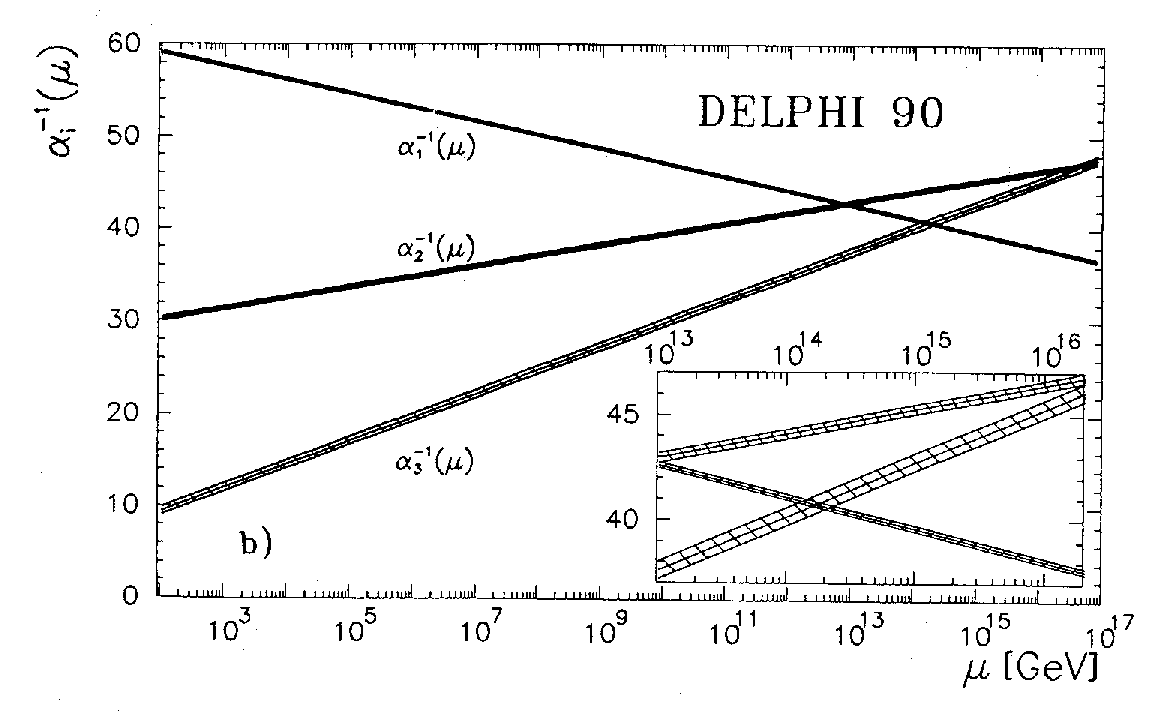
\includegraphics[width=0.49\textwidth]{figures/theory/running_couplings_SM}
      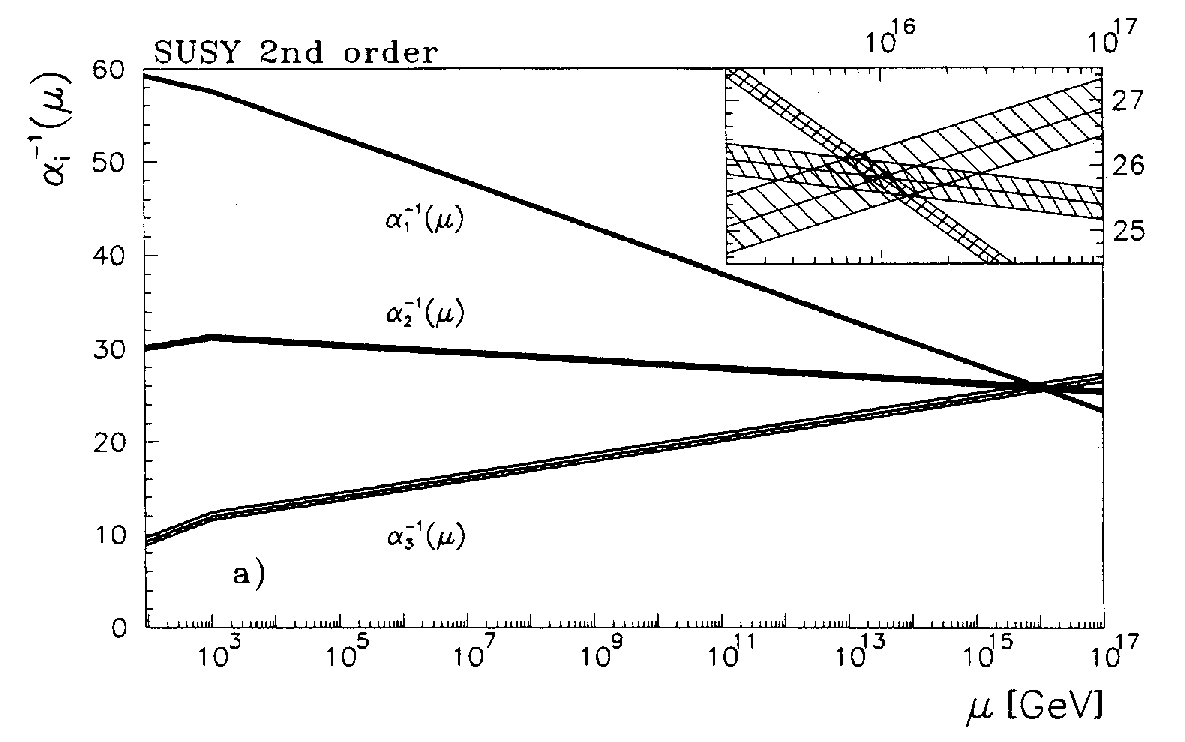
\includegraphics[width=0.49\textwidth]{figures/theory/running_couplings_MSSM}
  \caption{The running of the gauge couplings in the Standard Model (left) and in the minimal supersymmetric extension of the SM (right). Taken from~\cite{bib:Unification}.}  
  \label{fig:Unification}
\end{figure}

Besides these arguments, SUSY can also provide an answer to the problem of non-visible matter in the universe.
If the conservation of the so-called R-parity is required, the lightest supersymmetric particle (LSP) is stable.
If this particle is only weakly interacting, it can serve as a good candidate to explain fully or partially the sources of the relic density. 
R-parity is a multiplicative quantum number with 
\begin{equation}
\begin{aligned}
P_R & =  1 \qquad &&\text{SM particles}\\
P_R & = -1 &&\text{SUSY particles}.
\end{aligned}
\end{equation}
If R-parity is conserved, only terms are allowed in the Lagrangian density, that contain an even number of supersymmetric particles.
Therefore, no single SUSY particle can decay into only SM particles and thus, the LSP is stable.
The following discussions are restricted to R-parity conserving supersymmetric models.



\section{The MSSM}
\label{sec:MSSM}
The supersymmetric extension of the Standard Model with a minimal particle content is called the Minimal Supersymmetric Standard Model (MSSM).
In the following section, the particle content of the MSSM is introduced.

\subsection{The particle content of the MSSM}
In $\mathcal{N}=1$ supersymmetry, every SM particle has exactly one supersymmetric partner particle, which leads to a doubling of the particle content in the MSSM with respect to the SM\footnote{The supersymmetric partner particles of the fermions are called sfermions, whereas the partner particles of the gauge (Higgs) bosons are referred to as gauginos (higgsinos).}.
Additionally, it is necessary to introduce a second Higgs doublet to ensure the holomorphicity of the superpotential in the presence of mass terms for the up-type particles.
Furthermore, the MSSM only stays free from anomalies if there is a further Higgs doublet~\cite{bib:SUSYPrimer}.
This leads to the fact, that in the MSSM, there are five Higgs bosons instead of only one as in the SM.

\renewcommand{\arraystretch}{1.5}
\begin{table}[!b]
\centering
\caption{Chiral supermultiplets in the MSSM.}
\label{tab:chiral_multiplets}
\makebox[0.99\textwidth]{
\begin{tabular}{l|c|c|c}
\multicolumn{4}{c}{} \\
\toprule
                     &   spin 0                                     & spin $\frac{1}{2}$              & $SU(3)_C,\ SU(2)_L,\ U(1)_Y$\\ 
\midrule
   squarks/quarks    & $\left(\tilde{u}_L,\tilde{d}_L \right)$      & $\left(u_L,d_L\right)$           & $\mathbf{3},\ \mathbf{2},\ +\frac{1}{3}$\\ \cline{2-4}  
                     & $\tilde{\bar{u}}_L = \tilde{u}_R^{\dagger} $   & $\bar{u}_L = (u_R)^c$            & $\mathbf{\bar{3}},\ \mathbf{1},\ -\frac{4}{3}$\\ \cline{2-4}  
                     & $\tilde{\bar{d}}_L = \tilde{d}_R^{\dagger}$    & $\bar{d}_L = (d_R)^c$            & $\mathbf{\bar{3}},\ \mathbf{1},\ +\frac{2}{3}$\\ 
\midrule
   sleptons/leptons  & $\left(\tilde{\nu}_{eL},\tilde{e}_L\right)$   & $\left(\nu_{eL},e_L\right)$      & $\mathbf{1},\ \mathbf{2},\ -1$\\ \cline{2-4} 
                     & $\tilde{\bar{e}}_L = \tilde{e}_R^{\dagger}$    & $\bar{e}_L = (e_R)^c$            & $\mathbf{\bar{1}},\ \mathbf{1},\ +2$\\ 
\midrule
   Higgs/higgsinos   & $\left(H_u^+,H_u^0\right)$        & $\left(\tilde{H}_u^+,\tilde{H}_u^0\right)$   & $\mathbf{1},\ \mathbf{2},\ +1$\\ \cline{2-4}
                     & $\left(H_d^0,H_d^-\right)$        & $\left(\tilde{H}_d^0,\tilde{H}_d^-\right)$   & $\mathbf{1},\ \mathbf{2},\ -1$ \\ 
\bottomrule
\multicolumn{4}{c}{} 
\end{tabular}}
\end{table}  
\renewcommand{\arraystretch}{1.5}
\begin{table}[!b]
\centering
\caption{Vector supermultiplets in the MSSM.}
\label{tab:vector_multiplets}
\makebox[0.99\textwidth]{
\begin{tabular}{l|c|c|c}
\multicolumn{4}{c}{} \\
\toprule
                      &   spin $\frac{1}{2}$                                  & spin 1                 & $SU(3)_C,\ SU(2)_L,\ U(1)_Y$\\ 
\midrule
   gluinos/gluons     & $\tilde{g}$                       & $g$                 & $\mathbf{8},\ \mathbf{1},\ 0$\\ 
\midrule
   winos/$W$-bosons   & $\tilde{W}^{\pm},\ \tilde{W}^0$  & $W^{\pm},\ W^0$     & $\mathbf{1},\ \mathbf{3},\ 0$\\
\midrule
   bino/$B$-boson     & $\tilde{B}$                      & $B$                 & $\mathbf{1},\ \mathbf{1},\ 0$ \\  
\bottomrule
\multicolumn{4}{c}{}
\end{tabular}}
\end{table} 
In supersymmetry, all particles and their partner particles are described by so-called supermultiplets.
Since the generators of the gauge group commute with the generators of supersymmetry, all particles within one supermultiplet have same quantum numbers, besides the spin.
In a renormalisable theory, there are two different types of supermultiplets: chiral multiplets, which contain a two-component Weyl spinor describing the fermionic degrees of freedom and a complex scalar field for the bosonic degrees of freedom; vector multiplets containing a vector field and a two-component Weyl spinor.
The complete particle content of the MSSM is depicted in Tables~\ref{tab:chiral_multiplets} and~\ref{tab:vector_multiplets}. 
Since in supersymmetric theories only left-handed Weyl spinors appear in the Lagrangian density, the right-handed particles are described as charge conjugated spinors of the left-handed spinors.





\subsection{The Lagrangian density of the MSSM}
\label{sec:Lagrange_MSSM}
In the following, only the most important parts of the MSSM Lagrangian density will be described.
For a complete description of the Lagrangian density, the reader is again referred to~\cite{bib:Drees_2004}.

\subsubsection*{The superpotential}
The superpotential of the MSSM contains the self interaction terms of the Higgs bosons and generates the interaction terms of the Higgs bosons with the fermions and their superpartners.
As already noted, it is very common to assume R-parity conservation.
Hence, no terms appear in the Lagrangian that would violate lepton or baryon number conservation and the lightest supersymmetric particle is stable.
Thus, all possible terms are
\begin{equation}
\label{eq:SPMSSM}
 W_{\text{MSSM}} = \mu H_u \cdot H_d - Y_u^{ij} H_u \cdot Q_L^i u_R^{c\,j} + Y_d^{ij} H_d \cdot Q_L^i d_R^{\,c\,j} + Y_e^{ij} H_d \cdot L_L^i e_R^{c\,j},
\end{equation}
with the dot product defined as in~\cite{bib:Aitchison_2005} 
\begin{equation}
 A \cdot B = \epsilon^{\alpha\beta} A_{\alpha} B_{\beta} = A_1 B_2 - A_2 B_1.
\end{equation}

\subsubsection*{The soft-breaking Lagrangian density}
Since supersymmetry is broken, explicit SUSY breaking terms are added to the Lagrangian density.
In order not to introduce new sources of quadratic divergencies, only bilinear and trilinear terms appear in the soft-breaking Lagrangian
\begin{equation}
 \begin{split}
  - \mathcal{L}^{MSSM}_{soft} =\,& m_{H_u}^2 H_u^{\dagger} \cdot H_u +m_{H_d}^2 H_d^{\dagger} \cdot H_d + \left(B\mu\, H_u \cdot H_d + h.c.\right) \\
  & + m_{\tilde{Q}\,ij}^2 \tilde{Q}_{L\,i}^{\dagger} \cdot \tilde{Q}_{L\,j}+ m_{\tilde{u}\,ij}^2 \tilde{u}_{R\,i}^{c\,\dagger} \cdot \tilde{u}_{R\,j}^c
+ m_{\tilde{d}\,ij}^2 \tilde{d}_{R\,i}^{\,c\,\dagger} \cdot \tilde{d}_{R\,j}^{\,c}\\
& + m_{\tilde{L}\,ij}^2 \tilde{L}_{L\,i}^{\dagger} \cdot \tilde{L}_{L\,j}+ m_{\tilde{e}\,ij}^2 \tilde{e}_{R\,i}^{\,c\,\dagger} \cdot \tilde{e}_{R\,j}^{\,c}\\
& +\left(- \left( A_u Y_u \right)_{ij} H_u \cdot \tilde{Q}_{L\,i} \tilde{u}_{R\,j}^c +\left( A_d Y_d \right)_{ij} H_d \cdot \tilde{Q}_{L\,i} \tilde{d}_{R\,j}^{\,c} \right.\\
& \left. +\left( A_e Y_e \right)_{ij} H_d \cdot \tilde{L}_{L\,i} \tilde{e}_{R\,j}^{\,c} + h.c. \right)\\
& + \left(M_1 \tilde{B} \tilde{B} + M_2 \tilde{W}_a \tilde{W}_a + M_3 \tilde{g}_i \tilde{g}_i + h.c \right)
 \end{split}
\label{eq:SoftTerms}
\end{equation}
The first line contains mass terms for the Higgs bosons, the second and third line for the sfermions.
In the fourth and fifth line the trilinear couplings between the Higgs bosons and the sfermions appear.
Finally, the last line gives rise to mass terms for the gauginos (gluinos, winos, bino).

Because of the soft-breaking terms, the MSSM contains more than 100 free parameters.
Constraining the MSSM is thus a difficult task and usually in experimental particle physics, constrained versions of the MSSM or assumptions at the GUT scale are used to report the impact of searches on SUSY. 
In the following a short introduction of the phenomenological MSSM is given.
With its reduced parameter space, it allows to elaborate on long-lived particles in the MSSM in a much easier way.

\subsection{The phenomenological MSSM}
\label{subsec:pMSSM}
The phenomenological MSSM (pMSSM) imposes constraints that are reasonable in the sense that the pMSSM fulfils current observations and still keeps the phenomenological variety of the MSSM~\cite{bib:pMSSM}.
The following assumptions are imposed (in~\cite{bib:pMSSM} more detailed information about these assumptions can be found):
\begin{itemize}
\item No new sources of CP violation,
\item No flavour changing neutral currents,
\item First and second generation universality.
\end{itemize}
These assumption reduce the number of SUSY parameters to only 19.
The remaining free parameters are the following:
\begin{itemize}
\item $\tan \beta$ (the ratio of the vacuum expectation values of the two Higgs doublets)
\item $M_A$ (the mass of the pseudo-scalar Higgs boson)  
\item $\mu$ (the Higgs mass parameter)
\item $M_1$,$M_2$,$M_3$ (bino, wino and gluino mass parameters, respectively)
\item $m_{\tilde{q}}$, $m_{\tilde{l}}$, $m_{\tilde{u}}$, $m_{\tilde{d}}$ and $m_{\tilde{e}}$ (the first and second generation mass parameters)
\item  $m_{\tilde{Q}}$, $m_{\tilde{L}}$, $m_{\tilde{t}}$, $m_{\tilde{b}}$ and $m_{\tilde{\tau}}$ (the third generation mass parameters)
\item $A_t$, $A_b$ and $A_{\tau}$ (third generation trilinear couplings).
\end{itemize}

\section{Supersymmetry breaking}
As already noted, the mechanism of supersymmetry breaking is unknown.
There exist, however, several ideas how to spontaneously break supersymmetry.
All mechanisms have in common that they need to happen at high energies in a hidden sector.
``Messenger'' particles are introduced which mediate the breaking to the TeV scale.
This, however, implies that supersymmetry breaking is a question of extraordinary high energies and one can parametrise the breaking by the soft breaking terms introduced in Section~\ref{sec:Lagrange_MSSM}.

The most popular breaking mediation mechanisms are gravity-mediated supersymmetry breaking~\cite{bib:GravityMediation} and gauge-mediated supersymmetry breaking~\cite{bib:GaugeMediation}.

\chapter{Long-lived particles in the MSSM}
\label{ch:Longlived_Particles}
There are various mechanisms how particles can be long-lived, such as small couplings or (almost) conserved quantum numbers.
For a comprehensive review, the reader is referred to~\cite{bib:LonglivedParticles_Overview}.

In this thesis, the focus is set on particles that have a long lifetime due to a small decay phase space. 
A phase space suppression is possible when the mass splitting between the decaying particle and one of the decay products is very small.
In Part~\ref{part:analysis}, a search for highly ionising, short tracks is presented.
This search is motivated by long-lived charginos, that are nearly mass-degenerate with the lightest supersymmetric particle, the neutralino.
The underlying mechanism of this mass-degeneracy in the MSSM will be addressed in the next paragraphs.

In the MSSM, the lightest chargino (\chipm) and the lightest neutralino (\chiO) can be almost mass-degenerate, if the wino mass parameter ($M_2$) is smaller than the bino ($M_1$) and higgsino ($\mu$) mass parameters.
This can be seen from the chargino and neutralino mass matrices.
The chargino mass matrix in the basis $\Psi^+_i= \left(-i \tilde{W}^+,\tilde{h}_u^+  \right)$ and \mbox{$\Psi^-_i= \left(-i \tilde{W}^-,\tilde{h}_d^-  \right)$} is given by 
\begin{flalign}
\label{eq:CharginoMassMatrix}
\mathcal{M}_{\Psi^{\pm}} = 
\begin{pmatrix} 
M_2    & g v_d                    \\
g v_u  & \mu                  
\end{pmatrix}.
\end{flalign} 
The mass eigenstates can be deduced with the help of orthogonal matrices $V$ and $U$, \mbox{$\chi^+_i=V_{ij}\Psi^+_j$} and \mbox{$\chi^-_i = U_{ij} \Psi^-_j$}.

The neutralino mass matrix in the basis  $\Psi_i^0= \left(-i\tilde{B},-i\tilde{W}^0,\tilde{h}_u^0,\tilde{h}_d^0\right)$ is
\begin{flalign}
\label{eq:NeutralinoMassMatrix}
\mathcal{M}_{\Psi^0} = 
\begin{pmatrix} 
M_1                     & 0                       & \frac{g'v_u}{\sqrt{2}}  & -\frac{g'v_d}{\sqrt{2}}  \\
0                       & M_2                     & -\frac{g v_u}{\sqrt{2}} & \frac{g v_d}{\sqrt{2}}   \\
\frac{g'v_u}{\sqrt{2}}  & -\frac{g v_u}{\sqrt{2}} & 0                       & -\mu                     \\
-\frac{g'v_d}{\sqrt{2}} & \frac{g v_d}{\sqrt{2}}  & -\mu                    &  0                      
\end{pmatrix}.
\end{flalign}
The mass matrix can be diagonalised with an orthogonal matrix $N$ leading to four different mass eigenstates of $\tilde{\chi}^0_i = N_{ij} \Psi_j^0  $.

It can be easily seen from the mass matrices~\eqref{eq:CharginoMassMatrix} and~\eqref{eq:NeutralinoMassMatrix}, that in first order approximation - neglecting the off-diagonal elements which are of electroweak strength - the lightest chargino and the lightest neutralino are both wino-like for $M_2 < M_1,\mu$ with a mass of $m_\chi \simeq M_2$. 
Thus, the mass difference between \chipm and \chiO is only determined by higher order corrections: radiative corrections as well as tree-level mixing with other states.\\

%The following expressions are approximate neutralino and chargino mass terms for $M_2 \mu > m_W^2 \sin 2\beta$ and $|M_2 \pm \mu|$, $|M_1 \pm \mu| \gg m_Z$ (taken from~\cite{bib:PAS:CMS:pMSSM_2013})
%\begin{align}
%\label{eq:gaugino_masses}
%\begin{split}
%m_{\tilde{B}}    &\simeq  M_1   + \frac{m_Z^2 \left( M_1 + \mu \sin 2\beta  \right) \sin^2 \theta_W}{M_1^2 - \mu^2} \\
%m_{\tilde{W}}    &\simeq  M_2   + \frac{m_Z^2 \left( M_2 + \mu \sin 2\beta  \right) \cos^2 \theta_W}{M_2^2 - \mu^2} \\
%m_{\tilde{H}_1^0} &\simeq  |\mu| + \frac{m_Z^2 \left( 1 - \sin 2\beta \right) \left( \mu + M_2 \sin^2 \theta_W + M_1 \cos^2 \theta_W \right) sqn\left(\mu \right)}{2 \left(\mu +M_2 \right)\left(\mu +M_1 \right)} \\
%m_{\tilde{H}_2^0} &\simeq  |\mu| + \frac{m_Z^2 \left( 1 + \sin 2\beta \right) \left( \mu - M_2 \sin^2 \theta_W - M_1 \cos^2 \theta_W \right) sqn\left(\mu \right)}{2 \left(\mu -M_2 \right)\left(\mu -M_1 \right)} 
%\end{split}
%\end{align}
%\begin{align}
%\label{eq:chargino_masses}
%\begin{split}
%m_{\tilde{W}^{\pm}} &\simeq  M_2  + m_W^2 \left[ \frac{M_2 + \mu \sin 2\beta}{M_2^2 - \mu^2} \right]\\
%m_{\tilde{H^{\pm}}} &\simeq  |\mu|  + m_W^2 sgn\left( \mu \right) \left[ \frac{\mu + M_2 \sin 2\beta}{\mu^2 - M_2^2} \right]
%\end{split}
%\end{align}
%It is obvious from Eqs.~\ref{eq:gaugino_masses} and~\ref{eq:chargino_masses}, that if $M_2 < M_1,\, |\mu|$, the lightest neutralino state is wino-like and is fully mass-degenerate on tree level with the lightest chargino.


Furthermore, recent analyses of the pMSSM parameter space~\cite{bib:pMSSMScan_2013,bib:pMSSMScan_2012} show, that models with almost pure wino-like neutralinos as LSPs mostly come along with wino-like charginos being the next-to lightest supersymmetric particle (NLSP).
In~\cite{bib:pMSSMScan_2013}, a parameter scan in the pMSSM parameter space is performed, flat in the 19 different SUSY parameters.
Afterwards, the generated 3 million pMSSM models are confronted with theoretical constraints as well as experimental observations.
Theoretical constraints are \eg requiring stable vacua and no colour- or charge breaking minima.
Furthermore, the agreement with precision electroweak data, heavy flavour physics and collider results from LEP, Tevatron and LHC is required.
The accordance with relic density data is only implemented as an upper bound.
Phenomenological MSSM models that survive these constraints and have a wino-like neutralino as lightest supersymmetric particle, do frequently contain  a metastable chargino.
In a fraction of $\sim 25\%$ of these models, the metastable chargino decays inside the tracker, calorimeter or muon chamber.
The mass splitting between chargino and neutralino in these scenarios is typically of the order of $\sim160\mev$~\cite{bib:pMSSMScan_2013}.

Furthermore, a study has been performed within~\cite{bib:CMS:DT_8TeV} which interpretes the results of various beyond Standard Model searches in terms of the fraction of excluded parameter points in the pMSSM.
This study shows, that lifetimes between $1\cm \lesssim c\tau \lesssim 30\cm$ could not yet been accessed by any of the existing searches (cf. Fig.~\ref{fig:pMSSMplot} in Section~\ref{sec:Motivation}).



\section{Previous searches and constraints from indirect searches}

Several previous searches are sensitive on SUSY scenarios with almost mass-degenerate wino-like charginos and neutralinos.
In the following an overview about these previous searches will be given.

\subsection*{Searches at LEP}
Several searches at LEP were hunting for almost mass-degenerate neutralino-chargino scenarios~\cite{bib:PreviousSearches_ALEPH,bib:PreviousSearches_OPAL,bib:PreviousSearches_DELPHI_2003,bib:PreviousSearches_DELPHI}.
These searches were looking for events with a high-energetic initial state radiated photon leading to missing energy in events with chargino-pair production and invisible decay products.
The excluded parameter regions by these searches can be found in~\cite{bib:LEP:SUSY_results} and are depicted in Fig.~\ref{fig:LEP}.
The searches were interpreted for $M_1$ and $M_2$ almost degenerate and with a large unified scalar mass $m_0$ leading to sneutrino masses larger than 500\gev. 
Charginos are excluded up to a mass of 92.4\gev~\cite{bib:LEP:SUSY_results}.
\begin{figure}[!h]
  \centering
      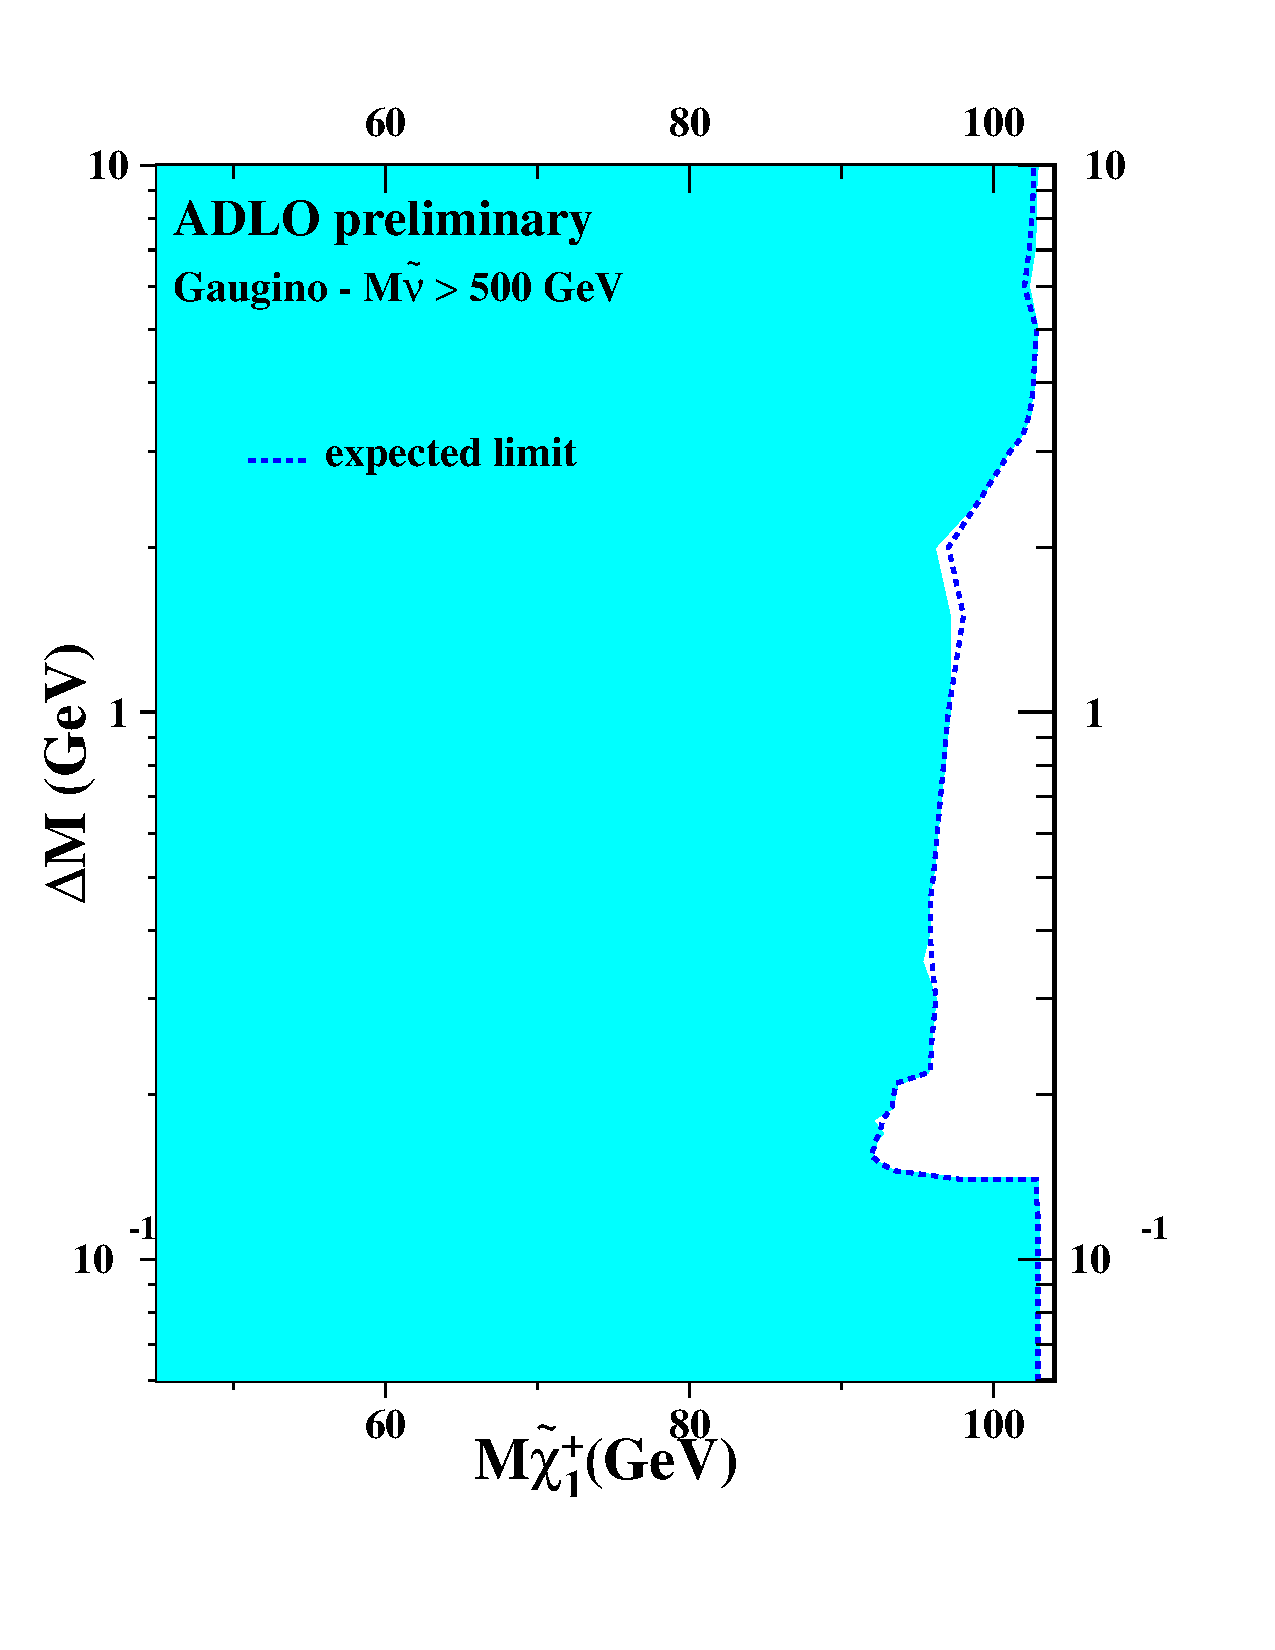
\includegraphics[width=0.45\textwidth]{figures/theory/mass_adlo_gaug_1.pdf}
  \caption{Observed and expected exclusion limits by LEP searches in the $m_{\chipm}-\Delta m \left( \chipm, \chiO \right)$ plane for almost degenerate $M_1$ and $M_2$ and a large unified scalar mass $m_0$. Taken from~\cite{bib:LEP:SUSY_results}.}  
  \label{fig:LEP}
\end{figure}

\subsection*{Searches at ATLAS at 7 and 8\tev}
At the ATLAS experiment at the LHC, searches for events with a disappearing track signature were performed at $\sqrt{s}=7\tev$~\cite{bib:PreviousSearches_Atlas_DT_7TeV} as well as at $\sqrt{s}=8\tev$~\cite{bib:PreviousSearches_Atlas_DT_8TeV}. 
Furthermore, a search for metastable particles with high ionisation losses was performed with $\sqrt{s}=8\tev$ data~\cite{bib:PreviousSearches_ATLAS_DEDX}.
These searches were interpreted within an anomaly-mediated supersymmetry breaking model~\cite{bib:Theory_AMSB_1998} with $\tan\beta=5$ and $\mu>0$.
The excluded parameter space by these searches is shown in Fig.~\ref{fig:ATLAS}.
Models with charginos down to lifetimes of 0.06\ns could be excluded.


\subsection*{Searches at CMS at 7 and 8\tev}
There are several searches at the CMS experiment at the LHC that are sensitive to long-lived wino-like charginos.
Among them is the search for long-lived charged particles~\cite{bib:CMS:HSCP_8TeV}, which searched for heavy particles with large energy deposits in the tracker at $\sqrt{s}=7\tev$  and $\sqrt{s}=8\tev$.
Furthermore, there is the search for disappearing tracks~\cite{bib:CMS:DT_8TeV} which analysed events with disappearing tracks in the tracker with respect to wino-like charginos almost mass-degenerate with the lightest neutralino.
This search was performed at the CMS experiment at a centre-of mass energy of $\sqrt{s}=8\tev$.
Since the latter search is more sensitive to shorter lifetime, only the exclusion limits derived by this search are shown in Fig.~\ref{fig:CMS}.
The disappearing track search by CMS shows a very similar sensitivity as the searches done at the ATLAS experiment.

\begin{figure}[!h]
  \centering
      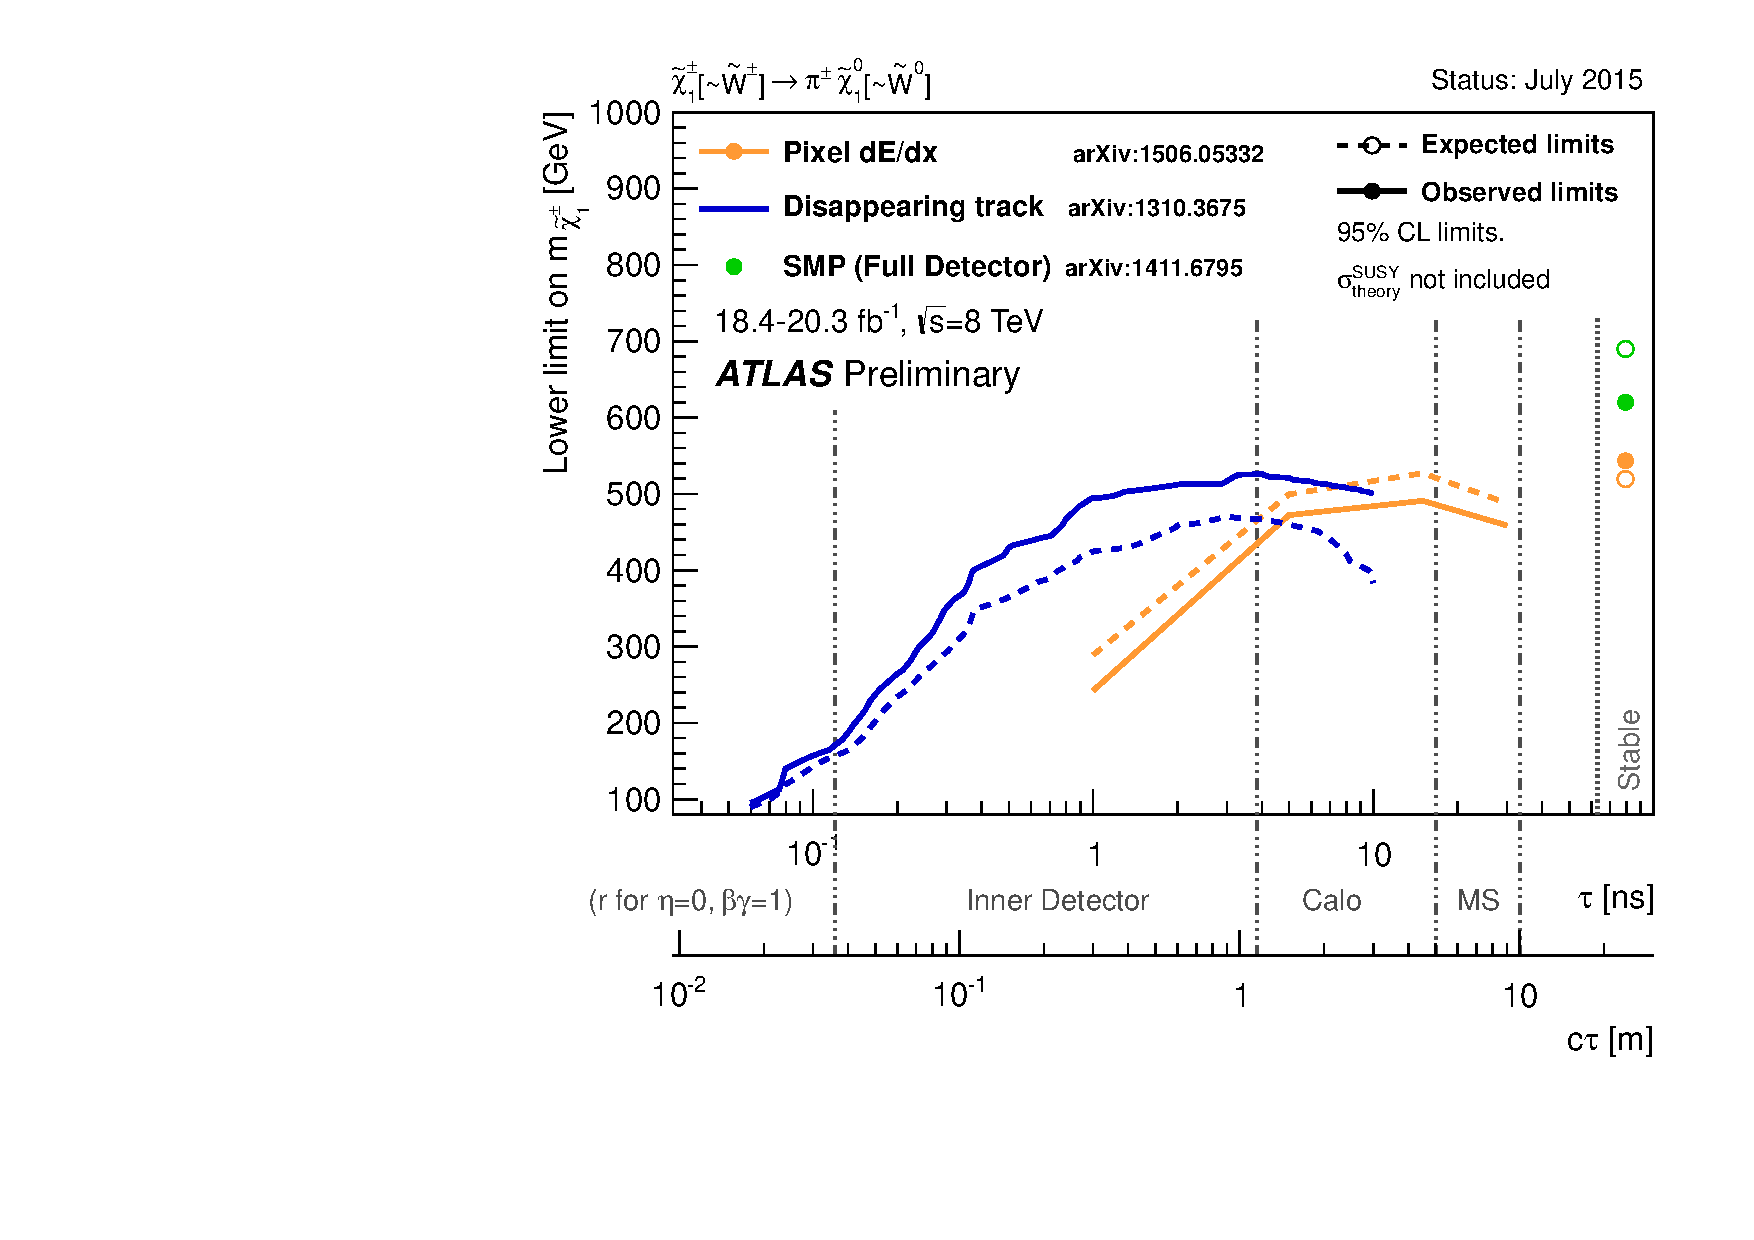
\includegraphics[width=0.54\textwidth]{figures/theory/ATLAS_SUSY_LLPChargino.pdf}
  \caption{Excluded parameter space by ATLAS searches in the $m_{\chipm}-\tau_{\chipm}$ plane for an AMSB model with $\tan\beta=5$ and $\mu>0$. Only chargino pair production is taken into account. The area below the curves is excluded. Taken from~\cite{bib:ATLAS_SUMMARYPLOTS}.}  
  \label{fig:ATLAS}
\end{figure}
\begin{figure}[!h]
  \centering
      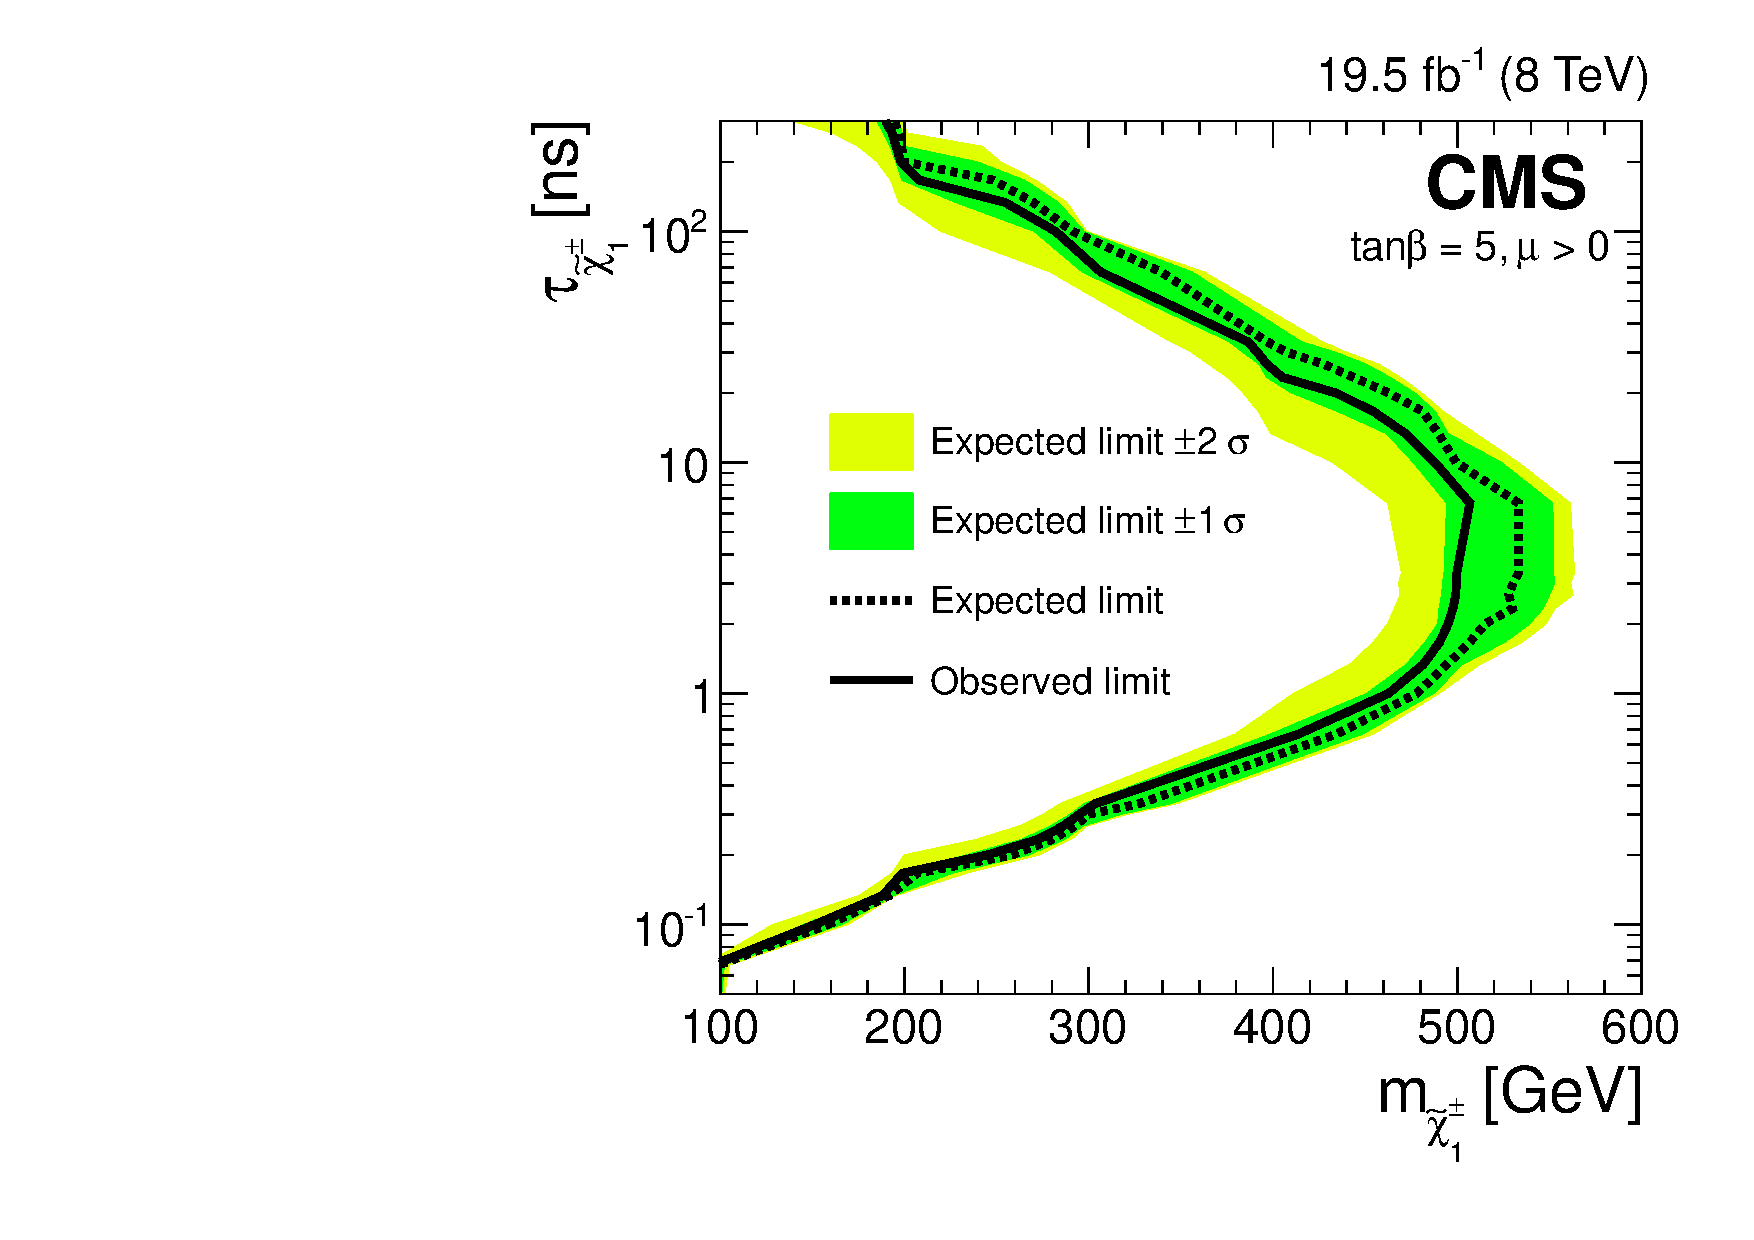
\includegraphics[width=0.54\textwidth]{figures/theory/lifetimeNs_vs_mass.pdf}
  \caption{Excluded parameter space by the Disappearing track search of CMS in the $\tau_{\chipm}-m_{\chipm}$ plane for wino-like charginos. The region left to the curve is excluded. Taken from~\cite{bib:CMS:DT_8TeV}.}  
  \label{fig:CMS}
\end{figure}

\subsection*{Indirect searches}
Finally, also results from indirect dark matter searches constrain the parameter region of SUSY models with wino-like charginos and neutralinos.
The most stringent limits are due to results by the Fermi Gamma-Ray Space Telescope (Fermi)~\cite{bib:Fermi} and the High Energy Spectroscopic System (H.E.S.S.)~\cite{bib:HESS}.

By the comparison of the observed gamma-ray signal to the theoretical prediction, Fermi sets upper limits on the dark matter annihilation cross-section considering six different decay channels~\cite{bib:Fermi_DM}.

H.E.S.S. sets upper limits on the DM annihilation cross section by the observation of the $\gamma$-ray line which is expected near the DM mass~\cite{bib:HESS_DM}.

Recent interpretations of the Fermi and H.E.S.S. data~\cite{bib:IndirectSearches_Fan_2013,bib:IndirectSearches_Cohen_2013,bib:IndirectSearches_Hryczuk_2014,bib:IndirectSearches_Beneke_2015} show that thermally produced wino-like neutralinos can only account for the full relic density for $\sim3.1\tev$~\cite{bib:IndirectSearches_Cohen_2013}, while DM masses between $1.6-3.0\tev$ are excluded by Fermi and H.E.S.S. observations.
Lower masses are still allowed, however, the neutralino cannot make up the full relic density.
%For scenarios with non-thermally produced neutralinos, the full mass region up to 3.1\tev is ruled out for scenarios where the wino-like neutralino is the only source of dark matter~\cite{bib:IndirectSearches_Cohen_2013}. 




% \chapter{Experimental setup/ Experiment and ... Experimental Setup: Collider, detector and algorithms } \label{sec:Detector}
% \section{LHC}
\section{CMS}
\section{Object reconstruction and particle identification}
\section{Event simulation}


% \chapter{Measurement of the jet transverse-momentum resolution} \label{sec:resolution}
% %%%%%%%%%%%%%%%%%%%%%%%%%%%%%%%%%%%%%%%%%%%%%%%%%%%%%%%%%%%%%%%%%%%%%%%%%%%%%%%%%%%%%%%%%%%%%%%%%%%%%%%%%%%%%%%%%%%%%%%%%%%%%%%%%%%%%%%%%%%%%%%%%%%%%%%%%%%%%%%%%%%%%%%%%%%%%%%%%%%%%%%%%%%%%%%%%%%%%%%%%%%%%%%%%%%%%%%%%%%%%%%%%%%%%%%%%%%
%%%%%%%%%%%%%%%%%%%%%%%%%%%%%%%%%%%%%%%%%%%%%%%%%%%%%%%%%%%%%%%%%%%%%%%%%%%%%%%%%%%%%%%%%%%%%%%%%%%%%%%%%%%%%%%%%%%%%%%%%%%%%%%%%%%%%%%%%%%%%%%%%%%%%%%%%%%%%%%%%%%%%%%%%%%%%%%%%%%%%%%%%%%%%%%%%%%%%%%%%%%%%%%%%%%%%%%%%%%%%%%%%%%%%%%%%%%
%%%%%%%%%%%%%%%%%%%%%%%%%%%%%%%%%%%%%%%%%%%%%%%%%%%%%%%%%%%%%%%%%%%%%%%%%%%%%%%%%%%%%%%%%%%%%%%%%%%%%%%%%%%%%%%%%%%%%%%%%%%%%%%%%%%%%%%%%%%%%%%%%%%%%%%%%%%%%%%%%%%%%%%%%%%%%%%%%%%%%%%%%%%%%%%%%%%%%%%%%%%%%%%%%%%%%%%%%%%%%%%%%%%%%%%%%%%
\chapter{Introduction}
\label{ch:Introduction}

The determination and quantification of the quality of the jet transverse momentum measurement is of crucial interest for many analyses with jet final states, 
\eg the measurement of the dijet cross section~\cite{bib:CMS:QCD_measurements} or $\ttbar$ production cross sections \cite{bib:CMS:TopCrossSection_8TeV}. 
Also searches for physics beyond the standard model with missing transverse momentum (\PTm) in the final state need a good knowledge of \PTm originating from wrongly measured jets \cite{}.
For analyses relying on information from simulation it is very important to correct the simulated resolution to the resolution actually present in data.
Therefore, scale factors will be presented to adjust the resolution in simulation to the resolution of the real detector.  
  
In the following sections, a data-based method to measure the jet \pt resolution in $\GAMJET$ events will be presented. 
A similar method was already accomplished in earlier analyses \cite{bib:CMS:JERCPaper_2011,bib:CMS-AN-2010-076,bib:CMS-AN-2010-141,bib:CMS-AN-2011-004} of 7\tev data.  
It is further developed here and applied to 8\tev data.

The method is based on the transverse momentum balance in the $\GAMJET$ system. 
It takes advantage of the high resolution of the electromagnetic calorimeter and hence the excellent measurement of the photon energy.
Without initial and final state radiation, the photon and the jet are balanced in the transverse plane. 
Thus, measuring the photon \pt with high accuracy leads to an estimate of the true jet transverse momentum offering a possibility to quantify the resolution of jet \pt measurements.


%%%%%%%%%%%%%%%%%%%%%%%%%%%%%%%%%%%%%%%%%%%%%%%%%%%%%%%%%%%%%%%%%%%%%%%%%%%%%%%%%%%%%%%%%%%%%%%%%%%%%%%%%%%%%%%%%%%%%%%%%%%%%%%%%%%%%%%%%%%%%%%%%%%%%%%%%%%%%%%%%%%%%%%%%%%%%%%%%%%%%%%%%%%%%%%%%%%%%%%%%%%%%%%%%%%%%%%%%%%%%%%%%%%%%%%%%%%
%%%%%%%%%%%%%%%%%%%%%%%%%%%%%%%%%%%%%%%%%%%%%%%%%%%%%%%%%%%%%%%%%%%%%%%%%%%%%%%%%%%%%%%%%%%%%%%%%%%%%%%%%%%%%%%%%%%%%%%%%%%%%%%%%%%%%%%%%%%%%%%%%%%%%%%%%%%%%%%%%%%%%%%%%%%%%%%%%%%%%%%%%%%%%%%%%%%%%%%%%%%%%%%%%%%%%%%%%%%%%%%%%%%%%%%%%%%
%%%%%%%%%%%%%%%%%%%%%%%%%%%%%%%%%%%%%%%%%%%%%%%%%%%%%%%%%%%%%%%%%%%%%%%%%%%%%%%%%%%%%%%%%%%%%%%%%%%%%%%%%%%%%%%%%%%%%%%%%%%%%%%%%%%%%%%%%%%%%%%%%%%%%%%%%%%%%%%%%%%%%%%%%%%%%%%%%%%%%%%%%%%%%%%%%%%%%%%%%%%%%%%%%%%%%%%%%%%%%%%%%%%%%%%%%%%
\chapter{General approach of the resolution measurement using photon+jet events}
\label{ch:GeneralApproach}

The jet transverse momentum resolution is defined as the standard deviation of the jet transverse momentum response distribution with the response 
defined as the ratio of the reconstructed to the true jet transverse momentum 
\begin{equation}\label{eq:responseFormula}
\mathcal{R} =  \frac{\pt^{\text{reco. jet}}}{\pt^{\text{true}}}.
\end{equation}
The jet transverse momentum resolution will be abbreviated JER throughout the following sections\footnote{This abbreviation is a historical relic from electron-position collider experiments where JER refered to jet energy resolution.}.

\mbox{Figure \ref{fig:TypicalResponse}} shows a typical response distribution for jets in the barrel region. 
\begin{figure}[t]
  \centering
      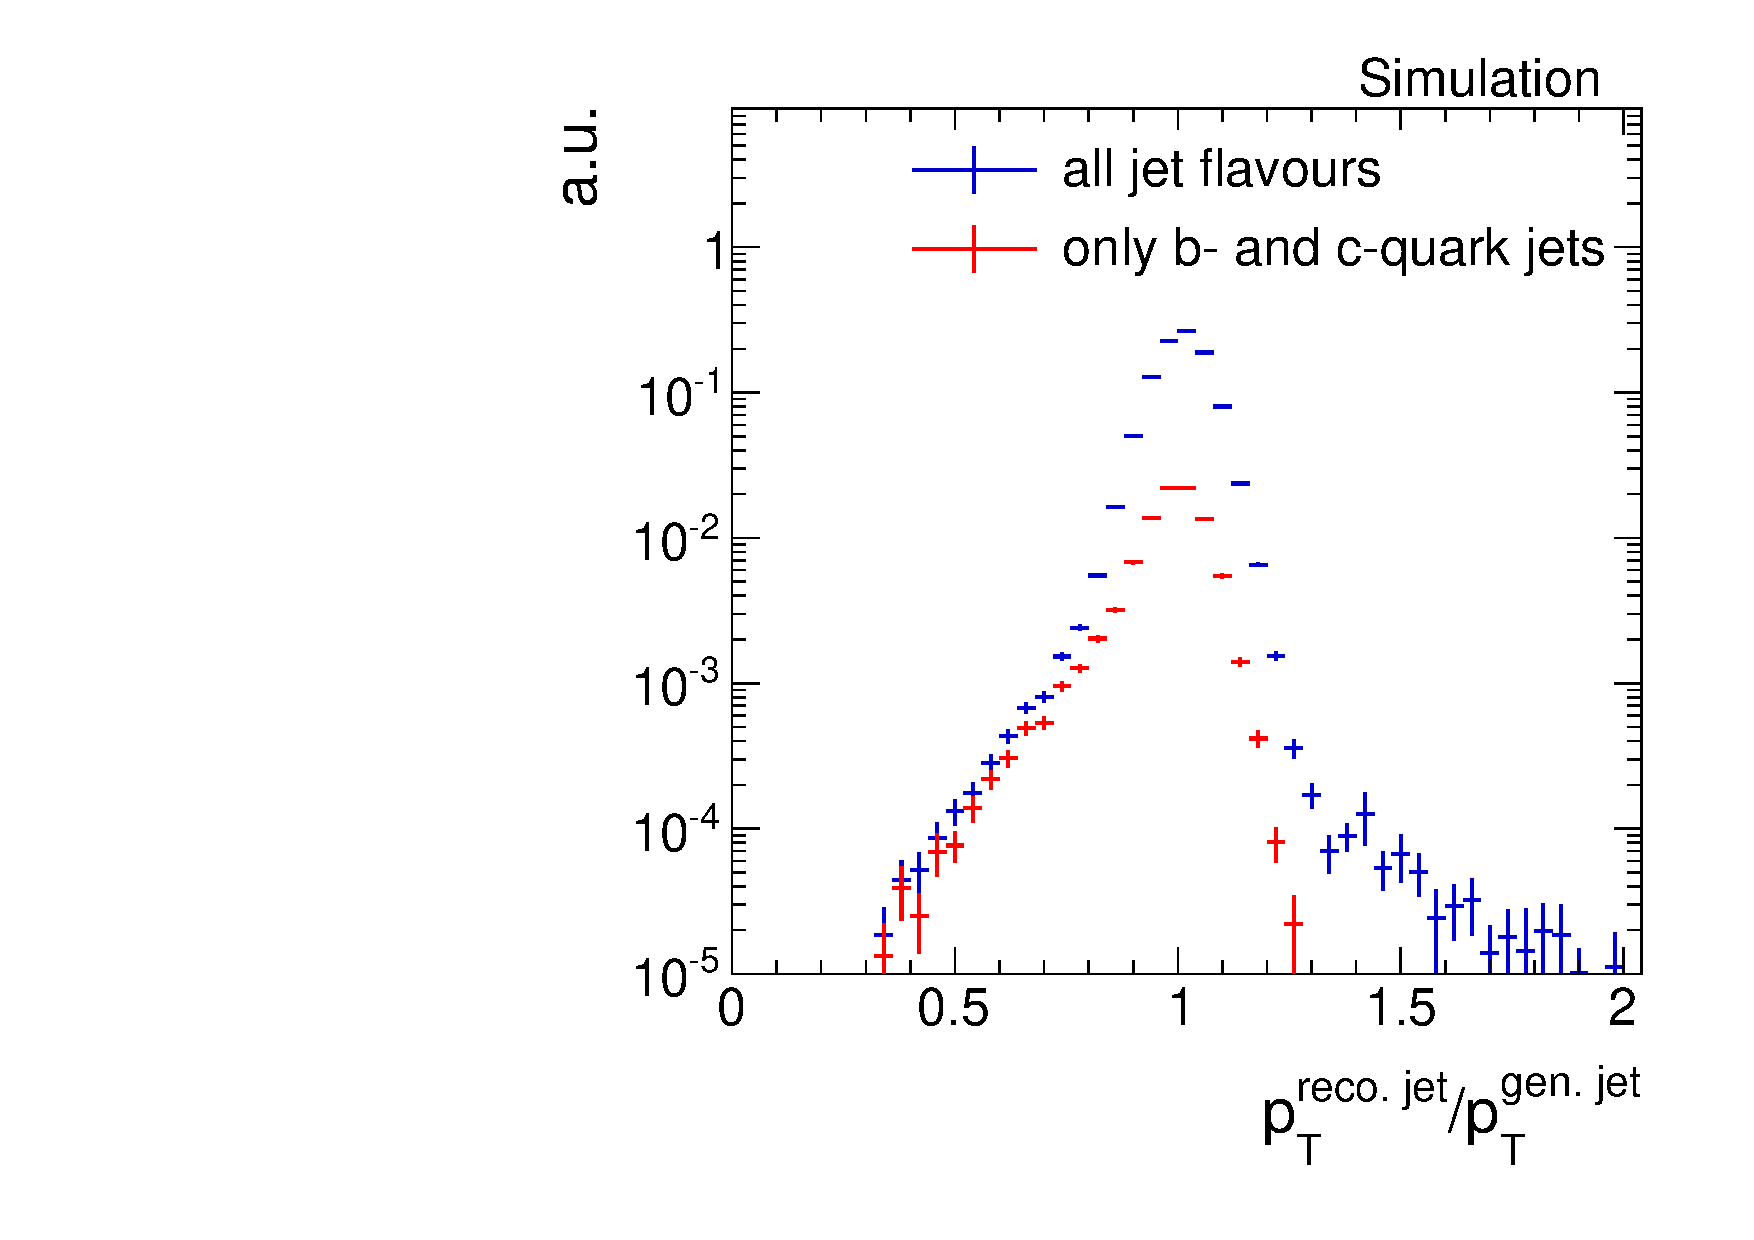
\includegraphics[width=0.49\textwidth]{figures/resolution/generalApproach/intrinsicExampleContributionofBCQuarks.pdf}
  \caption{Number of events over $\frac{\pt^{\text{reco. jet}}}{\pt^{\text{gen. jet}}}$ from a simulated $\GAMJET$ sample. 
           The black dots show the contribution by c- and b-quark jets where the left tail originating from semi-leptonic decays of heavy quarks can be seen.}  
  \label{fig:TypicalResponse}
\end{figure}
The core of the response distribution shows a Gaussian behavior whereas the tails deviate from that functional form.
Physical reasons for the low response tail are inter alia semi-leptonic decays of heavy quarks where the neutrino cannot be detected and the reconstructed transverse momentum of the jet is too small (see \mbox{Fig. \ref{fig:TypicalResponse}}). 
Some instrumental effects, such as a non-linear response of the calorimeter, inhomogeneities of the detector material and electronic noise can contribute to both tails, 
others, like dead calorimeter channels only contribute to the left tail. 
The resolution is therefore determined using only the core of the distribution to avoid the coverage of non-Gaussian tails.

Therefore, in this analysis note the resolution is defined as the standard deviation of the 99\% truncated response histogram devided by the mean of the histogram:

\begin{equation}\label{eq:resolutionFormula}
\text{JER} = \frac{\sigma_{99\%}}{\mu_{99\%}}.
\end{equation}

The determination of the 99\% range of the histogram is done in several steps. 
First the mean of the core is found via a Gaussian fit to the histogram in a 2$\sigma$ range \footnote{The 2$\sigma$ range is defined as the range [$\mu - 2\sigma$,$\mu + 2\sigma$].}. 
This procedure is done in three iteration steps.
Then, a symmetric interval around this mean is determined with its integral equal to 99\% of the integral of the full histogram. 

%The division by the mean is done to make the resolution measurement more insensitive to a variation of the jet energy scale (= mean of the response distribution)
%which has also an effect on the measured width of the distribution. 
%because response distributions with a scale smaller than one are typically narrower while distributions with scales larger than one are broader.

The evaluation of the response distribution as reconstructed over generated jet transverse momentum (\mbox{Eq.~\eqref{eq:responseFormula}})
is only possible for simulated events where generator information is accessible. 
A determination of the resolution in data, however, has to rely on a different approach.

The main idea of a resolution measurement using $\GAMJET$ events is based on the transverse momentum balance of the system and the excellent electromagnetic calorimeter resolution
(which was estimated between 1.1 \% and 2.6\% in the barrel region for photons for $\sqrt{s}= 7 \tev$ data \cite{bib:CMS:ECALresolution_7TeV} 
and is expected to be similar for $\sqrt{s}= 8 \tev$ data).

Several tree-level processes (\mbox{see Fig. \ref{fig:FeynmanDiagrams}}) lead to an event topology with one photon and one jet in the final state. 

\begin{figure}[htp]
  \centering

      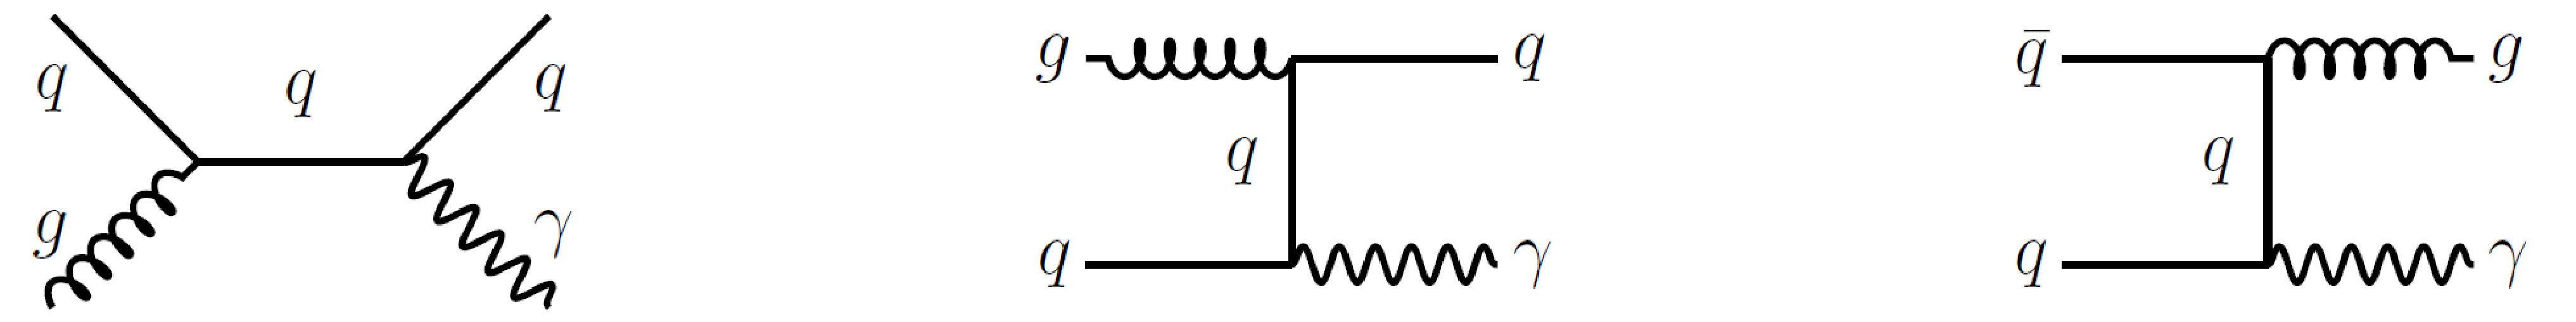
\includegraphics[width=0.99\textwidth]{figures/resolution/generalApproach/FeynmanDiagram.pdf}
 
 
  \caption{Tree-level Feynman diagrams of processes at the LHC in pp collisions with one photon and one jet in the final state.}  
  \label{fig:FeynmanDiagrams}
\end{figure}
Due to momentum conversation, the jet and the photon are back to back in the transverse plane, and therefore, $\vec{p}_{T}^{\gamma} = -\vec{p}_{T}^{\text{jet}}$. 
Because of the good resolution of the electromagnetic calorimeter, photon energies can be very well measured 
and thus can serve as an excellent estimator for the true jet energy.


Unfortunately, such clean events are very rare processes, and usually, the momentum balance is spoiled by initial and final state radiation, which lead to further jets in the event 
(see \mbox{Fig. \ref{fig:FeynmanDiagramsWithRadiation}}). 
However, in order to select events that are balanced to a large extent, a lower bound 
on the angular distance in the transverse plane between the photon and the jet with the highest transverse momentum (leading jet) is required ($\Delta\Phi>2.95\unit{rad}$). 

Additionally, the variable 

\begin{equation}\label{eq:alphaDef}
\alpha \doteq \frac{\pt^{\text{\nth{2} reco. jet}}}{\pt^{\gamma}}
\end{equation} 
is defined as a measure of further jet activity in an event. 
It is, however, not sufficient to require only an upper bound on $\alpha$. 
Instead, the jet energy resolution is measured in bins of $\alpha$ (with max($\alpha$) = 0.2), 
and the \mbox{extrapolated} value to zero further jet energy ($\alpha=0$) is taken as the measured resolution of the jet energy in the absence of further jets.


\begin{figure}[t]
  \centering

      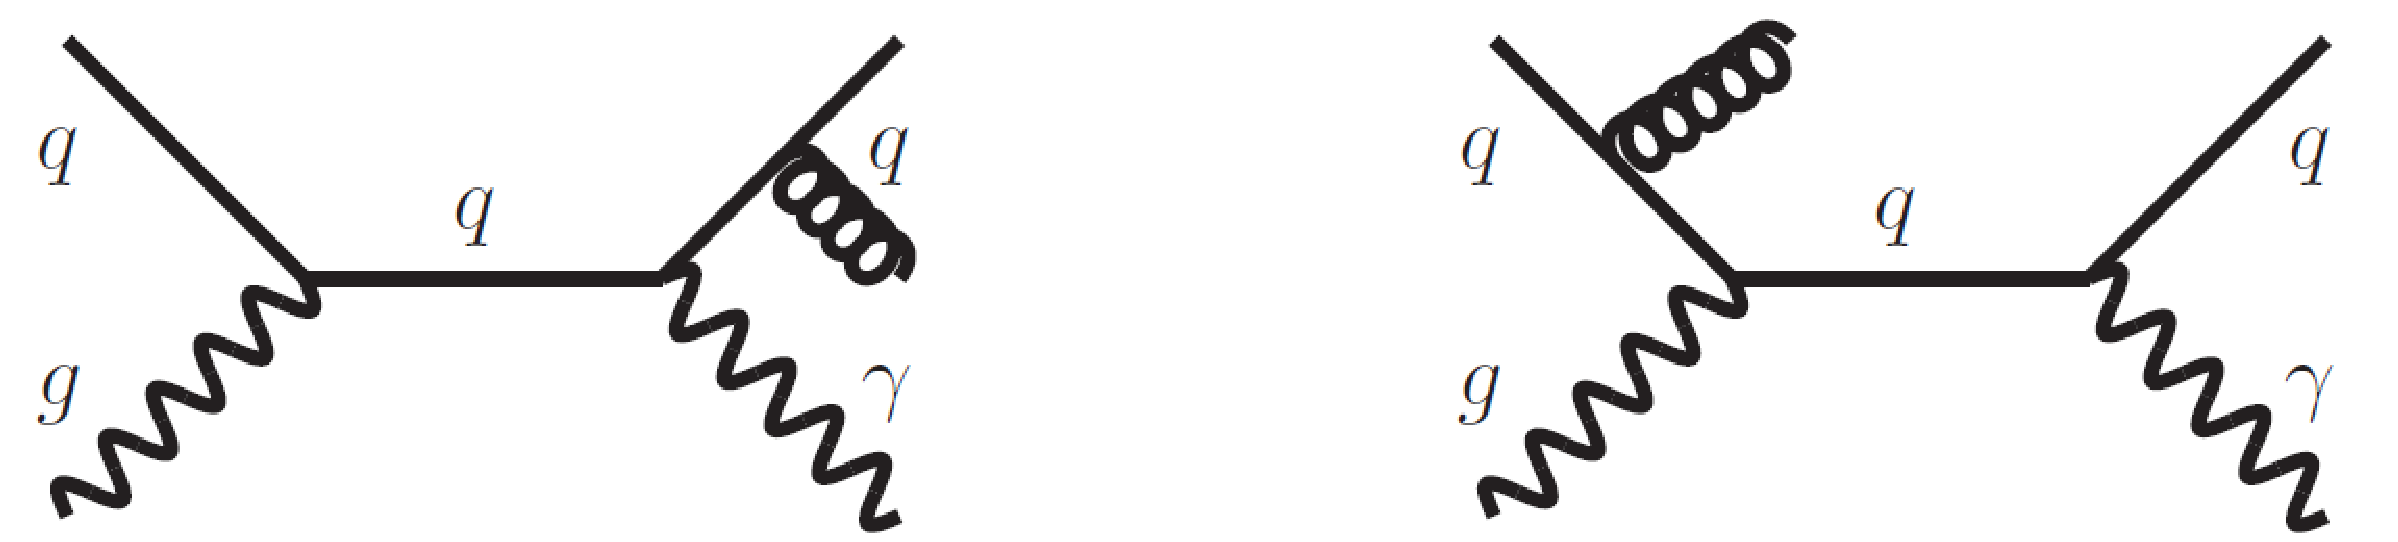
\includegraphics[width=0.60\textwidth]{figures/resolution/generalApproach/FeynmanDiagramsWithRadiation.pdf}
  
  \caption{Tree-level Feynman diagrams with initial and final state radiation.}  
  \label{fig:FeynmanDiagramsWithRadiation}
\end{figure}

Measuring the transverse momentum of the photon instead of taking the generator jet $p_{T}$ leads to the fact that the measured resolution consists out of two parts

\begin{equation}\label{eq:splitting}
\frac{\pt^{\text{reco. jet}}}{\pt^{\gamma}} = \underbrace{\frac{\pt^{\text{reco. jet}}}{\pt^{\text{gen. jet}}}}_{\text{intrinsic}} \cdot \underbrace{\frac{\pt^{\text{gen. jet}}}{\pt^{\gamma}}}_{\text{imbalance}}.
\end{equation}

The intrinsic part is the resolution of interest which is independent of further jets in the event whereas the imbalance is strongly dependent on $\alpha$.

To extract the intrinsic resolution out of the measured one, the residual imbalance $q^{\prime}$ (the imbalance at $\alpha = 0$) is subtracted from the total resolution in the 
limit of vanishing additional jet activity. 
As that information is only available from simulation, the measured resolution in data is corrected by the residual imbalance taken from the simulated data set.
%%%%%%%%%%%%%%%%%%%%%%%%%%%%%%%%%%%%%%%%%%%%%%%%%%%%%%%%%%%%%%%%%%%%%%%%%%%%%%%%%%%%%%%%%%%%%%%%%%%%%%%%%%%%%%%%%%%%%%%%%%%%%%%%%%%%%%%%%%%%%%%%%%%%%%%%%%%%%%%%%%%%%%%%%%%%%%%%%%%%%%%%%%%%%%%%%%%%%%%%%%%%%%%%%%%%%%%%%%%%%%%%%%%%%%%%%%%

%%%%%%%%%%%%%%%%%%%%%%%%%%%%%%%%%%%%%%%%%%%%%%%%%%%%%%%%%%%%%%%%%%%%%%%%%%%%%%%%%%%%%%%%%%%%%%%%%%%%%%%%%%%%%%%%%%%%%%%%%%%%%%%%%%%%%%%%%%%%%%%%%%%%%%%%%%%%%%%%%%%%%%%%%%%%%%%%%%%%%%%%%%%%%%%%%%%%%%%%%%%%%%%%%%%%%%%%%%%%%%%%%%%%%%%%%%%
%%%%%%%%%%%%%%%%%%%%%%%%%%%%%%%%%%%%%%%%%%%%%%%%%%%%%%%%%%%%%%%%%%%%%%%%%%%%%%%%%%%%%%%%%%%%%%%%%%%%%%%%%%%%%%%%%%%%%%%%%%%%%%%%%%%%%%%%%%%%%%%%%%%%%%%%%%%%%%%%%%%%%%%%%%%%%%%%%%%%%%%%%%%%%%%%%%%%%%%%%%%%%%%%%%%%%%%%%%%%%%%%%%%%%%%%%%%
\chapter{Datasets and event selection}

\begin{itemize}
\item  selection - take from AN
\end{itemize}

Pictures as root file available:
\begin{itemize}
\item BLA
\end{itemize}

Picture \textcolor{red}{NOT} as root file available:
\begin{itemize}
\item BLA
\end{itemize}
%%%%%%%%%%%%%%%%%%%%%%%%%%%%%%%%%%%%%%%%%%%%%%%%%%%%%%%%%%%%%%%%%%%%%%%%%%%%%%%%%%%%%%%%%%%%%%%%%%%%%%%%%%%%%%%%%%%%%%%%%%%%%%%%%%%%%%%%%%%%%%%%%%%%%%%%%%%%%%%%%%%%%%%%%%%%%%%%%%%%%%%%%%%%%%%%%%%%%%%%%%%%%%%%%%%%%%%%%%%%%%%%%%%%%%%%%%%

%%%%%%%%%%%%%%%%%%%%%%%%%%%%%%%%%%%%%%%%%%%%%%%%%%%%%%%%%%%%%%%%%%%%%%%%%%%%%%%%%%%%%%%%%%%%%%%%%%%%%%%%%%%%%%%%%%%%%%%%%%%%%%%%%%%%%%%%%%%%%%%%%%%%%%%%%%%%%%%%%%%%%%%%%%%%%%%%%%%%%%%%%%%%%%%%%%%%%%%%%%%%%%%%%%%%%%%%%%%%%%%%%%%%%%%%%%%
%%%%%%%%%%%%%%%%%%%%%%%%%%%%%%%%%%%%%%%%%%%%%%%%%%%%%%%%%%%%%%%%%%%%%%%%%%%%%%%%%%%%%%%%%%%%%%%%%%%%%%%%%%%%%%%%%%%%%%%%%%%%%%%%%%%%%%%%%%%%%%%%%%%%%%%%%%%%%%%%%%%%%%%%%%%%%%%%%%%%%%%%%%%%%%%%%%%%%%%%%%%%%%%%%%%%%%%%%%%%%%%%%%%%%%%%%%%
\chapter{Methodology of the measurement}

\begin{itemize}
\item Take from AN
\end{itemize}

Pictures as root file available:
\begin{itemize}
\item BLA
\end{itemize}

Picture \textcolor{red}{NOT} as root file available:
\begin{itemize}
\item BLA
\end{itemize}
%%%%%%%%%%%%%%%%%%%%%%%%%%%%%%%%%%%%%%%%%%%%%%%%%%%%%%%%%%%%%%%%%%%%%%%%%%%%%%%%%%%%%%%%%%%%%%%%%%%%%%%%%%%%%%%%%%%%%%%%%%%%%%%%%%%%%%%%%%%%%%%%%%%%%%%%%%%%%%%%%%%%%%%%%%%%%%%%%%%%%%%%%%%%%%%%%%%%%%%%%%%%%%%%%%%%%%%%%%%%%%%%%%%%%%%%%%%

%%%%%%%%%%%%%%%%%%%%%%%%%%%%%%%%%%%%%%%%%%%%%%%%%%%%%%%%%%%%%%%%%%%%%%%%%%%%%%%%%%%%%%%%%%%%%%%%%%%%%%%%%%%%%%%%%%%%%%%%%%%%%%%%%%%%%%%%%%%%%%%%%%%%%%%%%%%%%%%%%%%%%%%%%%%%%%%%%%%%%%%%%%%%%%%%%%%%%%%%%%%%%%%%%%%%%%%%%%%%%%%%%%%%%%%%%%%
%%%%%%%%%%%%%%%%%%%%%%%%%%%%%%%%%%%%%%%%%%%%%%%%%%%%%%%%%%%%%%%%%%%%%%%%%%%%%%%%%%%%%%%%%%%%%%%%%%%%%%%%%%%%%%%%%%%%%%%%%%%%%%%%%%%%%%%%%%%%%%%%%%%%%%%%%%%%%%%%%%%%%%%%%%%%%%%%%%%%%%%%%%%%%%%%%%%%%%%%%%%%%%%%%%%%%%%%%%%%%%%%%%%%%%%%%%%
\chapter{Systematic uncertainties}

\begin{itemize}
\item difficult to take from AN
\end{itemize}

Pictures as root file available:
\begin{itemize}
\item BLA
\end{itemize}

Picture \textcolor{red}{NOT} as root file available:
\begin{itemize}
\item BLA
\end{itemize}
%%%%%%%%%%%%%%%%%%%%%%%%%%%%%%%%%%%%%%%%%%%%%%%%%%%%%%%%%%%%%%%%%%%%%%%%%%%%%%%%%%%%%%%%%%%%%%%%%%%%%%%%%%%%%%%%%%%%%%%%%%%%%%%%%%%%%%%%%%%%%%%%%%%%%%%%%%%%%%%%%%%%%%%%%%%%%%%%%%%%%%%%%%%%%%%%%%%%%%%%%%%%%%%%%%%%%%%%%%%%%%%%%%%%%%%%%%%

%%%%%%%%%%%%%%%%%%%%%%%%%%%%%%%%%%%%%%%%%%%%%%%%%%%%%%%%%%%%%%%%%%%%%%%%%%%%%%%%%%%%%%%%%%%%%%%%%%%%%%%%%%%%%%%%%%%%%%%%%%%%%%%%%%%%%%%%%%%%%%%%%%%%%%%%%%%%%%%%%%%%%%%%%%%%%%%%%%%%%%%%%%%%%%%%%%%%%%%%%%%%%%%%%%%%%%%%%%%%%%%%%%%%%%%%%%%
%%%%%%%%%%%%%%%%%%%%%%%%%%%%%%%%%%%%%%%%%%%%%%%%%%%%%%%%%%%%%%%%%%%%%%%%%%%%%%%%%%%%%%%%%%%%%%%%%%%%%%%%%%%%%%%%%%%%%%%%%%%%%%%%%%%%%%%%%%%%%%%%%%%%%%%%%%%%%%%%%%%%%%%%%%%%%%%%%%%%%%%%%%%%%%%%%%%%%%%%%%%%%%%%%%%%%%%%%%%%%%%%%%%%%%%%%%%
\chapter{Results}

\begin{itemize}
\item THINK
\end{itemize}

Pictures as root file available:
\begin{itemize}
\item BLA
\end{itemize}

Picture \textcolor{red}{NOT} as root file available:
\begin{itemize}
\item BLA
\end{itemize}
%%%%%%%%%%%%%%%%%%%%%%%%%%%%%%%%%%%%%%%%%%%%%%%%%%%%%%%%%%%%%%%%%%%%%%%%%%%%%%%%%%%%%%%%%%%%%%%%%%%%%%%%%%%%%%%%%%%%%%%%%%%%%%%%%%%%%%%%%%%%%%%%%%%%%%%%%%%%%%%%%%%%%%%%%%%%%%%%%%%%%%%%%%%%%%%%%%%%%%%%%%%%%%%%%%%%%%%%%%%%%%%%%%%%%%%%%%%

%%%%%%%%%%%%%%%%%%%%%%%%%%%%%%%%%%%%%%%%%%%%%%%%%%%%%%%%%%%%%%%%%%%%%%%%%%%%%%%%%%%%%%%%%%%%%%%%%%%%%%%%%%%%%%%%%%%%%%%%%%%%%%%%%%%%%%%%%%%%%%%%%%%%%%%%%%%%%%%%%%%%%%%%%%%%%%%%%%%%%%%%%%%%%%%%%%%%%%%%%%%%%%%%%%%%%%%%%%%%%%%%%%%%%%%%%%%
%%%%%%%%%%%%%%%%%%%%%%%%%%%%%%%%%%%%%%%%%%%%%%%%%%%%%%%%%%%%%%%%%%%%%%%%%%%%%%%%%%%%%%%%%%%%%%%%%%%%%%%%%%%%%%%%%%%%%%%%%%%%%%%%%%%%%%%%%%%%%%%%%%%%%%%%%%%%%%%%%%%%%%%%%%%%%%%%%%%%%%%%%%%%%%%%%%%%%%%%%%%%%%%%%%%%%%%%%%%%%%%%%%%%%%%%%%%
\chapter{Discussion and conclusion}

\begin{itemize}
\item Repeat results
\item cross-check analysis
\item Outlook
\end{itemize}

Pictures as root file available:
\begin{itemize}
\item BLA
\end{itemize}

Picture \textcolor{red}{NOT} as root file available:
\begin{itemize}
\item BLA
\end{itemize}


\chapter{A search for highly ionizing, short tracks at the CMS detector} \label{sec:analysis}

In this chapter a search for highly ionizing, short tracks is presented. The chapter will be structured as follows:
In \mbox{Sec.~\ref{sec:Motivation}} a motivation will be given, followed by an overview of the general search strategy in \mbox{Sec.~\ref{sec:GeneralSearchStrategy}}.
As the variable \dedx plays a crucial role in this analysis, a general introduction and different possible parametrizations will be introduced in \mbox{Sec.~\ref{sec:DeDxMeasurement}}.
In this context also the conducted offline calibration of the silicon pixel detector will be explained.
After presenting the simulated SM and signal samples which were used in this analysis (\mbox{Sec.~\ref{sec:SimulatedSamples}}) the event selection is shown (Sec.~\ref{sec:EventSelection}).
Then, the various sources of background are charecterized (Sec.~\ref{sec:SourcesOfBackgrounds}) and the methods to estimate their size are presented (\ref{sec:BackgroundEstimation}).
As a final step an optimization in the search sensitivity was done, which can be found in Sec.~\ref{sec:Optimization}.
The chapter concludes by presenting the results of this analysis in Sec.~\ref{sec:Results}, and after a short introduction to the statistical methods of limit setting (Sec.~\ref{sec:LimitSetting}), the results will be interpreted in the context of Supersymmetry (Sec.~\ref{sec:Interpretation}).


%%%%%%%%%%%%%%%%%%%%%%%%%%%%%%%%%%%%%%%%%%%%%%%%%%%%%%%%%%%%%%%%%%%%%%%%%%%%%%%%%%%%%%%%%%%%%%%%%%%%%%%%%%%%%%%%%%%%%%%%%%%%%%%%%%%%%%%%%%%%%%%%%%%%%%%%%%%%%%%%%%%%%%%%%%%%%%%%%%%%
\section{Motivation}
\label{sec:Motivation}
As it was already pointed out in Chap.~\ref{ch:Theory}, Supersymmetry is able to offer solutions to unexplained phenomena in astrophysics and can solve the shortcomings of the Standard Model of particle physics.
Unfortunately, due to the unknown mechanism of supersymmetry breaking, the most general parametrization of Supersymmetry introduces over 100 new dimensions which opens up an incredibly huge phenomenalogically rich space, 
leading to very different possible signature at particle colliders. 
During the Phase\,I run at the LHC in 2012, a variety of different seaches, optimized on the hunt for supersymmetry were conducted.
At the CMS and at the ATLAS experiment, taking data from proton-ptoton collsions, a strong focus was put on the search for hints of SUSY in the strong production sector (e.g. \cite{bib:CMS:RA2_8TeV,bib:CMS:MT2_8TeV,bib:ATLAS:JetPlusMET_8TeV}).
This led already to a wide exclusion in SUSY space, which nevertheless still offers some very interesting non-excluded parameter regions.
The search for SUSY in more "exotic" regions gains therefore more and more attention. 
Typical SUSY scenarios which are not easily excluded by the general SUSY searches consists of so-called compressed spectra, where two or more particles are nearly degenerate in their masses.
When mother and daughter particles are almost mass-degenerate, the remaining decay product in a two body decay can be very soft in \pt, making those scenarios very challenging to search for.
Thus supersymmetric scenarios with compressed spectra are usually much weaker constrained than the corresponding scenarios without compressed spectra.\\

In this analysis the focus is put on the possiblity of a lightest chargino ($\chi^{\pm}_1$) which is almost mass degenerate with the lightest neutralino ($\chi^{0}_1$).
As shown in Sec.~\ref{theorySUSY}, long lifetimes are possible for various reasons.
The scenarios presented here lead to long lifetimes of the chargino because of phase space supression.

A chargino can be produced via chargino pair production through a photon or a Z boson exchange. The chargino decays then via a virtual W boson to the lightest neutralino and fermion-fermion pair (e.g. a pion).
This process is illustrated in the Feynman diagram shown in fig. \ref{fig:FeynmanDiagram}.

\begin{figure}[!tb]
  \centering 
  \begin{tabular}{c}
    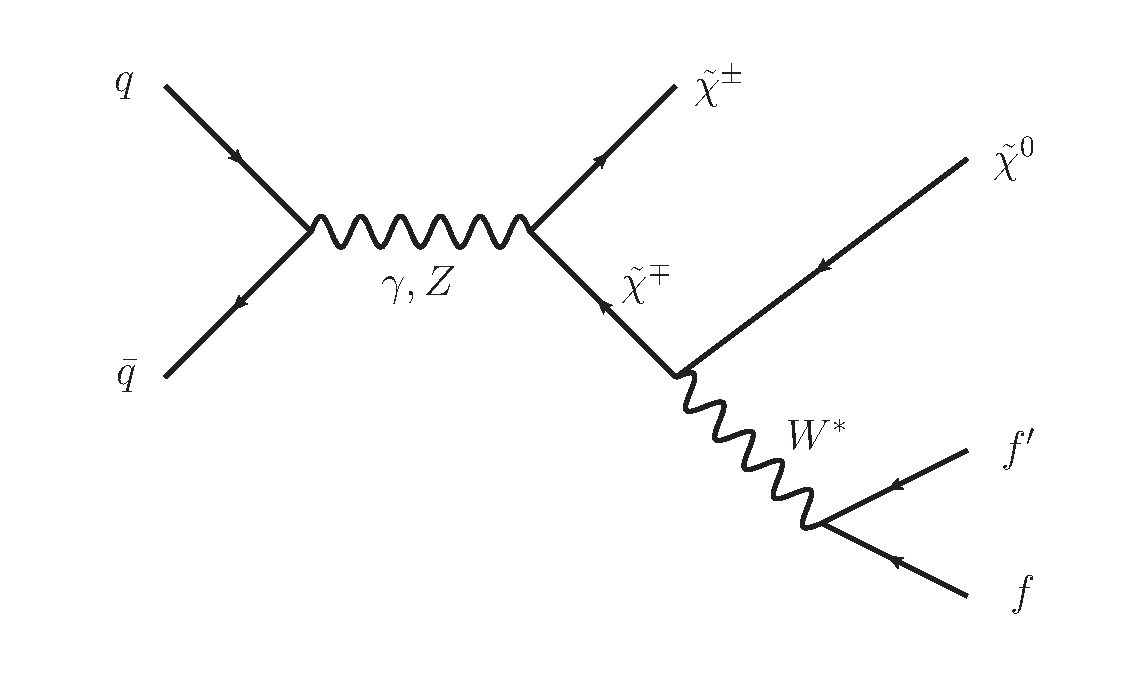
\includegraphics[width=0.75\textwidth]{figures/analysis/ChiChi_ProductionAndDecay.pdf}
  \end{tabular}
  \caption{Feynman diagram showing a possible production mechanism of a chargino pair and the decay channel of a chargino.}
  \label{fig:FeynmanDiagram}
\end{figure}

Other possible production channels are the exchange of a supersymmetric Higgs boson or via a t-channel squark exchange. 
The corresponding Feynman diagrams for the tree level production channels are shown in Fig.~\ref{fig:FeynmanDiagramProductionCharginoPair}.

\begin{figure}[!b]
  \centering 
  \begin{tabular}{c}
    \frame{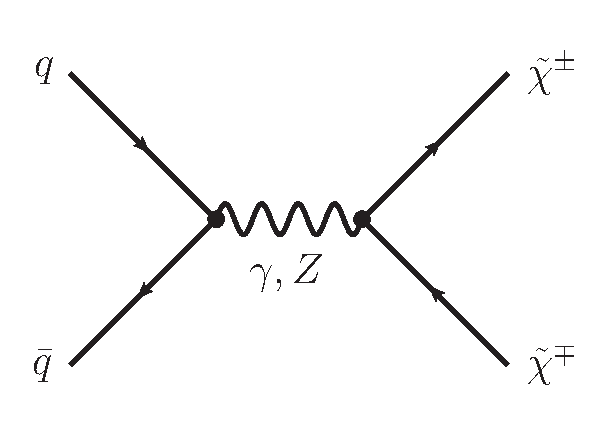
\includegraphics[width=0.33\textwidth]{figures/analysis/ChiChi_GammaZ.pdf}
    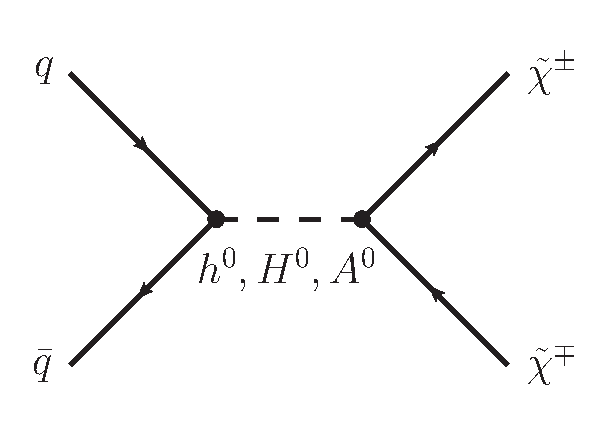
\includegraphics[width=0.33\textwidth]{figures/analysis/ChiChi_Scalar.pdf}
    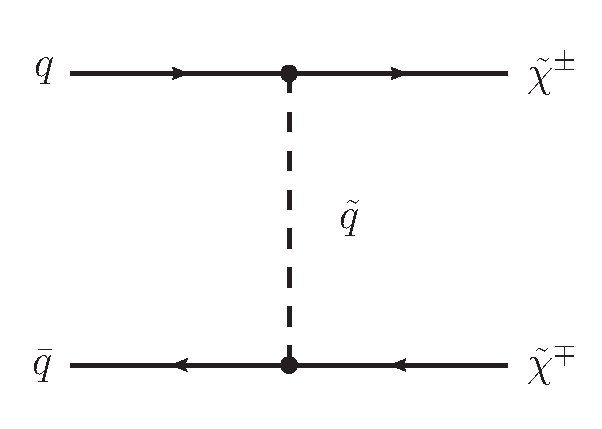
\includegraphics[width=0.33\textwidth]{figures/analysis/ChiChi_Squark.pdf}}
  \end{tabular}
  \caption{Main tree level diagrams for chargino pair production.}
  \label{fig:FeynmanDiagramProductionCharginoPair}
\begin{tabular}{c}
    \frame{    
    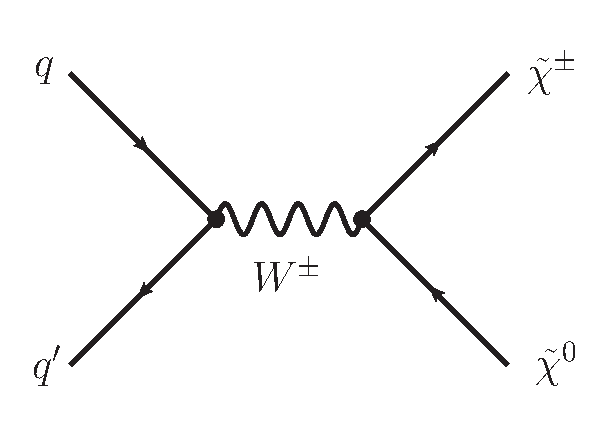
\includegraphics[width=0.33\textwidth]{figures/analysis/ChiChi0_WBoson.pdf}
    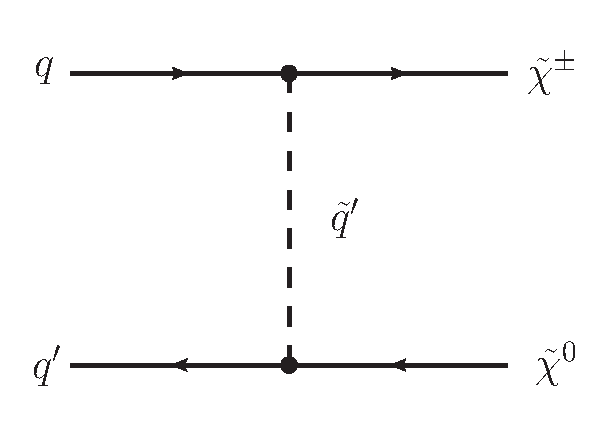
\includegraphics[width=0.33\textwidth]{figures/analysis/ChiChi0_Squark.pdf}
    }
  \end{tabular}
  \caption{Main tree level diagrams for chargino neutralino production.}
  \label{fig:FeynmanDiagramProductionCharginoNeutralino}
\end{figure}
Another possibility of chargino production is the chargino neutralino production channel. 
On tree level, there exist two production mechanism: the s-channel W boson exchange and the t-channel squark exchange, see Fig.~\ref{fig:FeynmanDiagramProductionCharginoNeutralino} for the Feynman diagrams.\\

Even if the presented supersymmetric model where $\chi^{\pm}_1$ and $\chi^{0}_1$ are nearly mass-degenerate leads to more exotic signatures at the CMS experiment, there have been already several analyses conducted in CMS which are in principle (even not all were designed to be) sensitive to these models.
Among those are a search for long-lived charged particles \cite{bib:CMS:HSCP_8TeV}, which was mainly designed for particles which have such a long lifetime that they travel through the full detector without decaying and a search for disappearing tracks \cite{bib:CMS:DT_8TeV} which looked for rather intermediate lifetimes, where the charginos decays already inside the tracker. 
Within \cite{bib:CMS:DT_8TeV}, a study was done, based on an interpretation exercise \cite{bib:CMS:HSCPReinterpreation_PAS} within the phenomenological MSSM (see Sec.~\ref{theorySUSY} for a detailed introduction to the pMSSM), which tests the exclusion power of various analyses done at CMS.

\begin{figure}[!b]
  \centering 
  \begin{tabular}{c}
    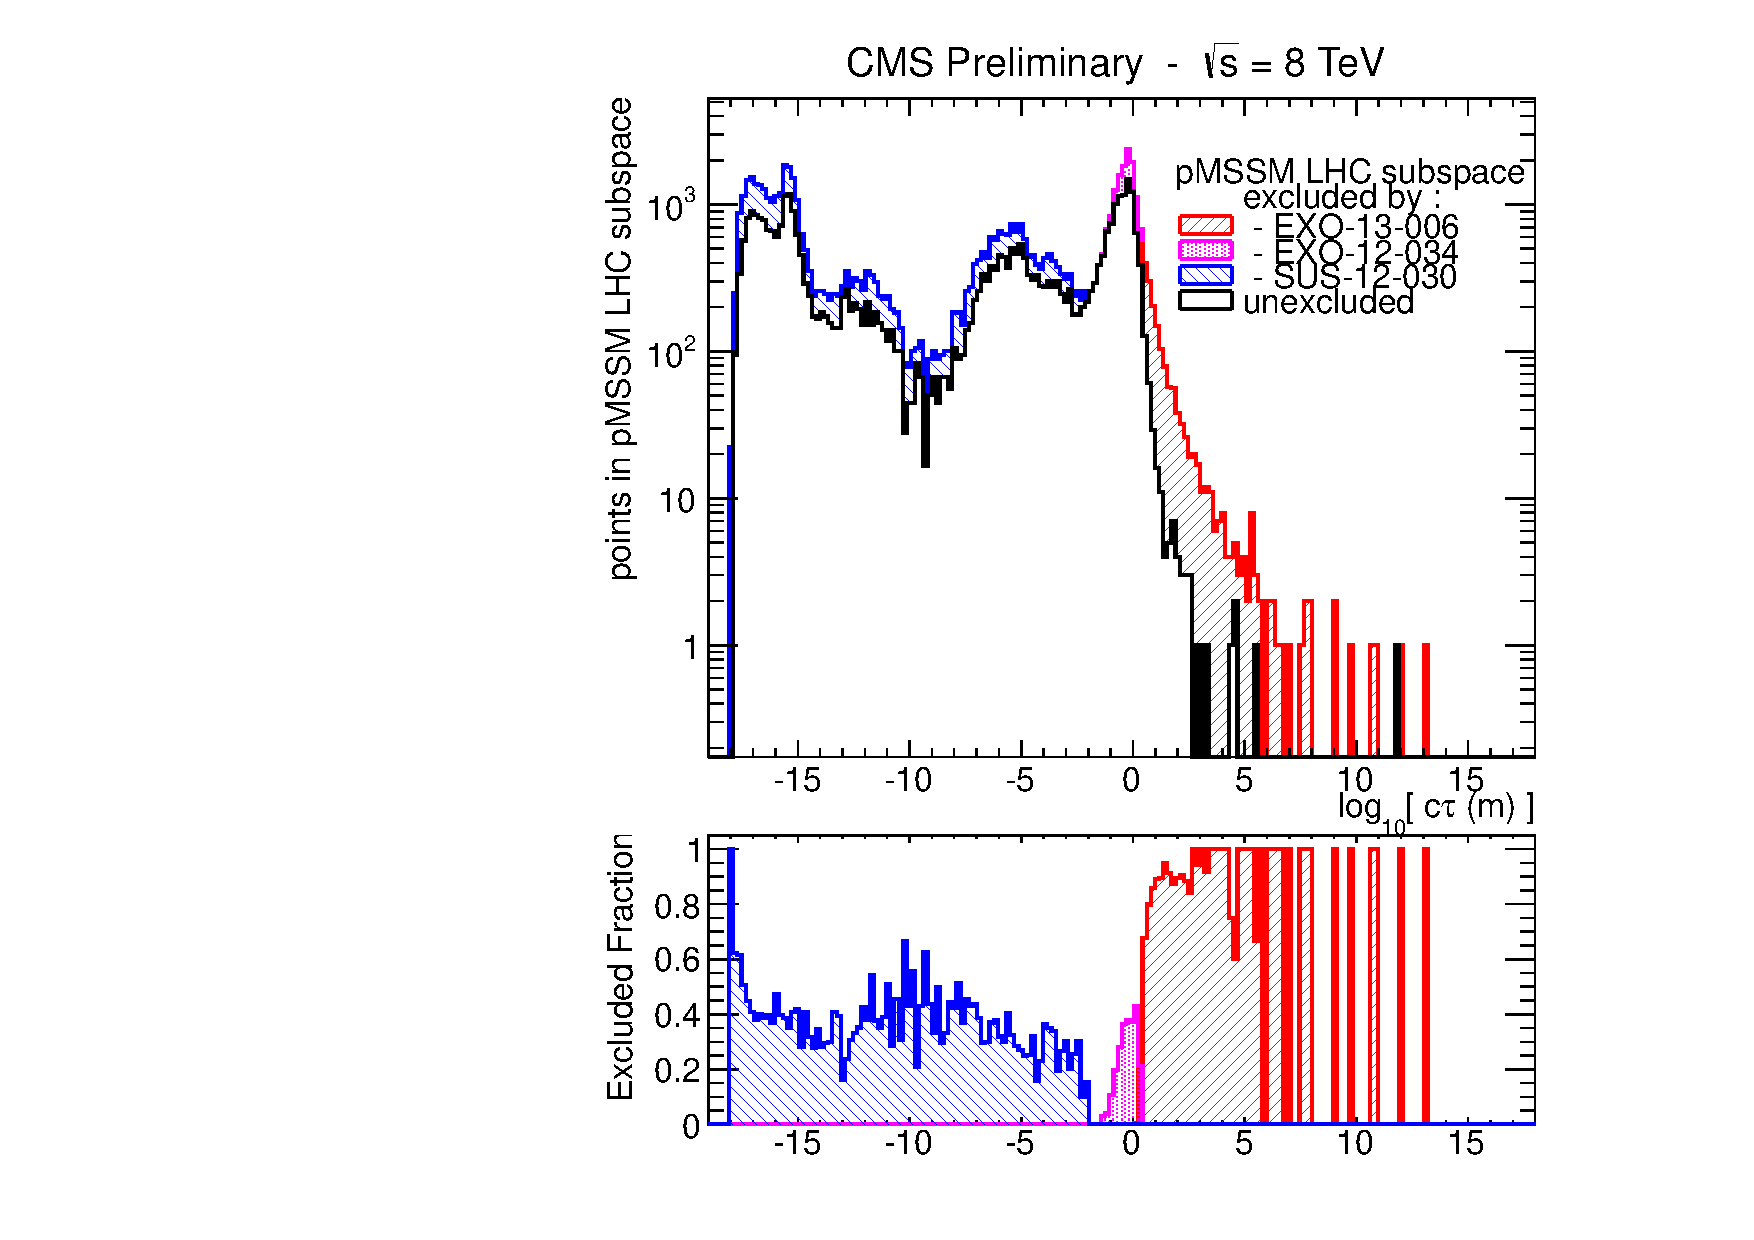
\includegraphics[width=0.75\textwidth]{figures/analysis/pMSSM_vs_ctau.pdf}
  \end{tabular}
  \caption{Exclusion power of various analyses dependent on chargino lifetime [c$\tau$]. Lower part of the plot shows the excluded fraction. Taken from: \href{https://twiki.cern.ch/twiki/bin/view/CMSPublic/PhysicsResultsEXO12034}{click here}.}
  \label{fig:pMSSMplot}
\end{figure}
In Fig.~\ref{fig:pMSSMplot}, the exclusion power of the search for long-live charged particles \cite{bib:CMS:HSCP_8TeV} in red, the search for diasappearing tracks \cite{bib:CMS:DT_8TeV} in purple and a collection of various SUSY analysis from \cite{bib:CMS:pMSSMinterpretation_7TeV_PAS} in blue over the chargino mass is shown. 
In black the distribution of the unexcluded pMSSM parameter points vs. the chargino mass can be seen.
The sampling of the parameter space points was done according to a pre-CMS likehood function, which takes into account electroweak precisicion measurements, etc.
In the lower part of Fig~\ref{fig:pMSSMplot}, the excluded fraction of pMSSM points is shown. 
It can be seen, that the more general SUSY searches are mostly sensitive to shorter chargino lifetimes ($c\tau \lesssim 10 \,\text{cm}$), whereas the search for long-lived particles shows very good sensitivity for lifetimes $>100\,$cm.
The search for disappearing tracks is sensitive on supersymmetric models with chargino lifetimes between $35\,\text{cm} \lesssim c\tau \lesssim 100\,\text{cm}$.

This analysis is targeting the gap between the disappearing track search (purple area) and the searches which are sensitive to instanteanously decaying charginos (blue area). The idea is to make use of the variable dE/dx which can be very discriminating for particles with high mass.
The challenges of such a search and the general strategy of this analysis will be presented int the next section.

%%%%%%%%%%%%%%%%%%%%%%%%%%%%%%%%%%%%%%%%%%%%%%%%%%%%%%%%%%%%%%%%%%%%%%%%%%%%%%%%%%%%%%%%%%%%%%%%%%%%%%%%%%%%%%%%%%%%%%%%%%%%%%%%%%%%%%%%%%%%%%%%%%%%%%%%%%%%%%%%%%%%%%%%%%%%%%%%%%%%
%%%%%%%%%%%%%%%%%%%%%%%%%%%%%%%%%%%%%%%%%%%%%%%%%%%%%%%%%%%%%%%%%%%%%%%%%%%%%%%%%%%%%%%%%%%%%%%%%%%%%%%%%%%%%%%%%%%%%%%%%%%%%%%%%%%%%%%%%%%%%%%%%%%%%%%%%%%%%%%%%%%%%%%%%%%%%%%%%%%%
\section{General search strategy}
\label{sec:GeneralSearchStrategy}

When searching for supersymmetric models with long-lived \chipm, the strategy is of course highly dependent on the actual lifetime of the chargino. 
For long lifetimes, the chargino can reach the muon chambers and can be reconstructed as a muon (even with a longer time-of-flight). 
For lower lifetimes, the chargino can already decay inside the detector (e.g. the tracker), thus not leading to a reconstructed muon in the event, but only to an isolated track in the tracker. 
The detector signatures of these two scenarios are visualised in Fig~\ref{fig:CharginoPaiEventDisplay}, where in a cross-sectional view of the CMS detector simulated chargino-chargino events are shown.
\begin{figure}[!b]
  \centering 
  \begin{tabular}{c}
    \frame{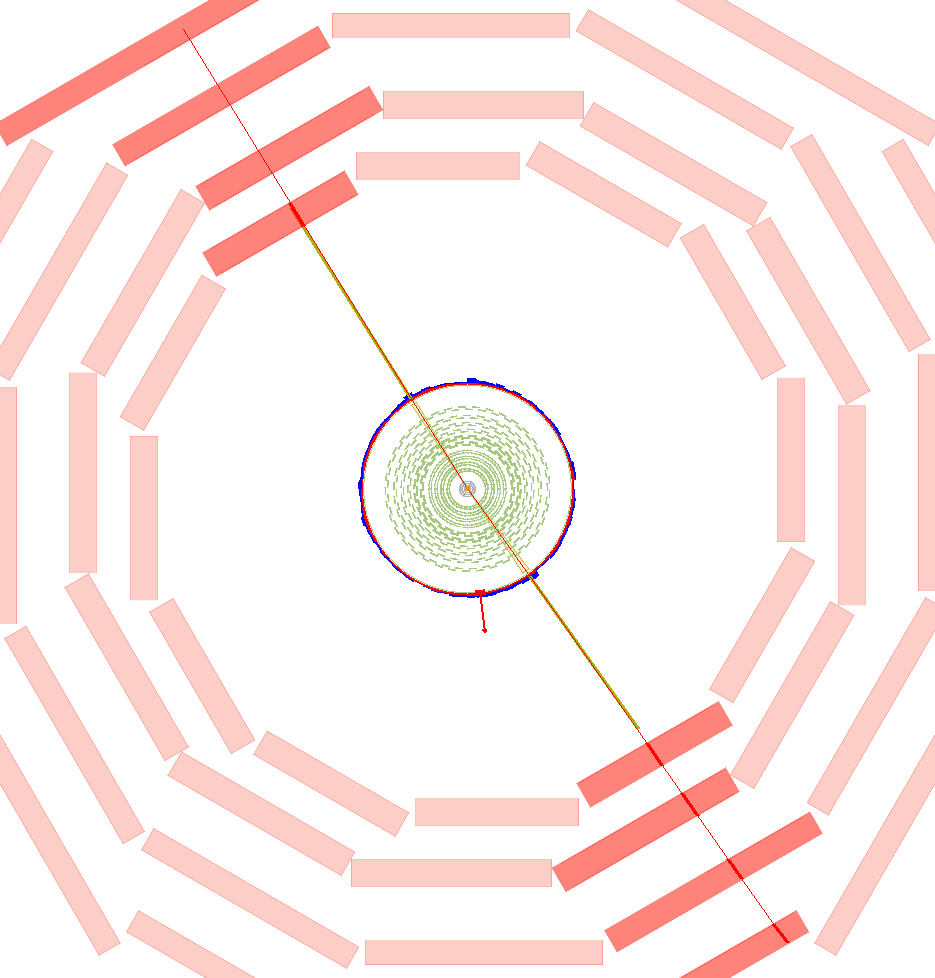
\includegraphics[width=0.31\textwidth]{figures/analysis/EventDisplay_scenario1.png}}
    \frame{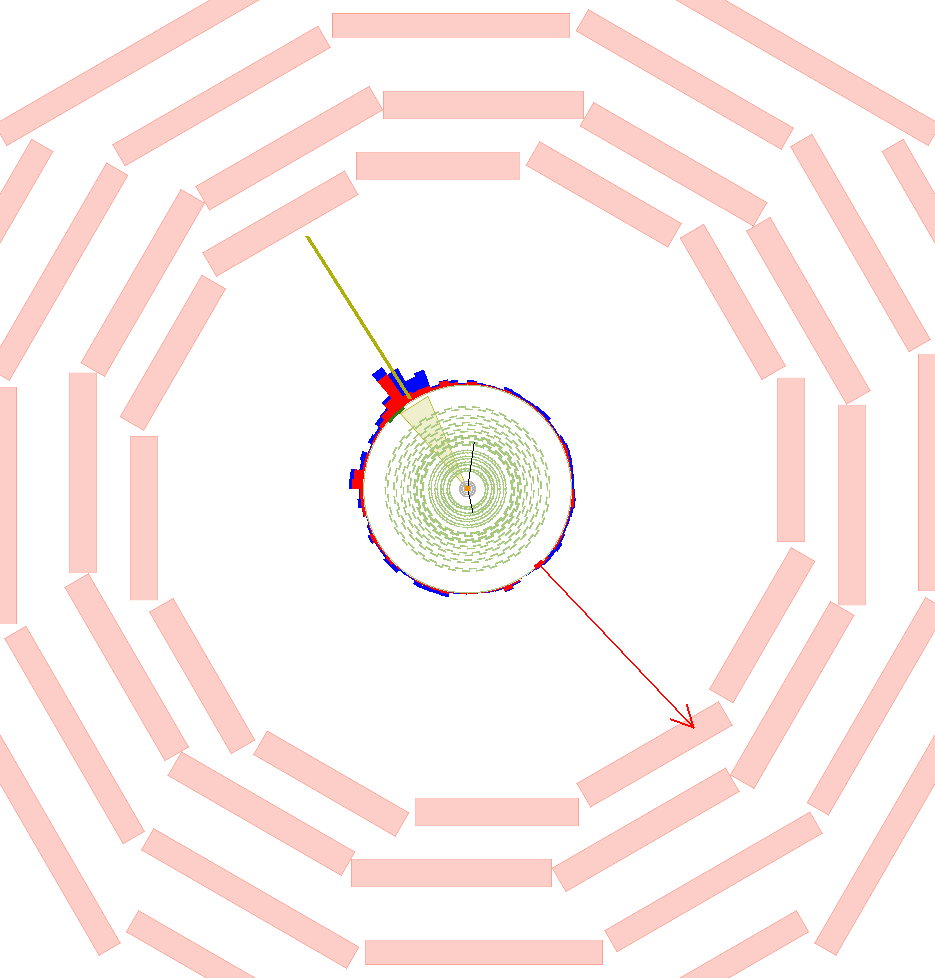
\includegraphics[width=0.31\textwidth]{figures/analysis/EventDisplay_scenario2.png}}
    \frame{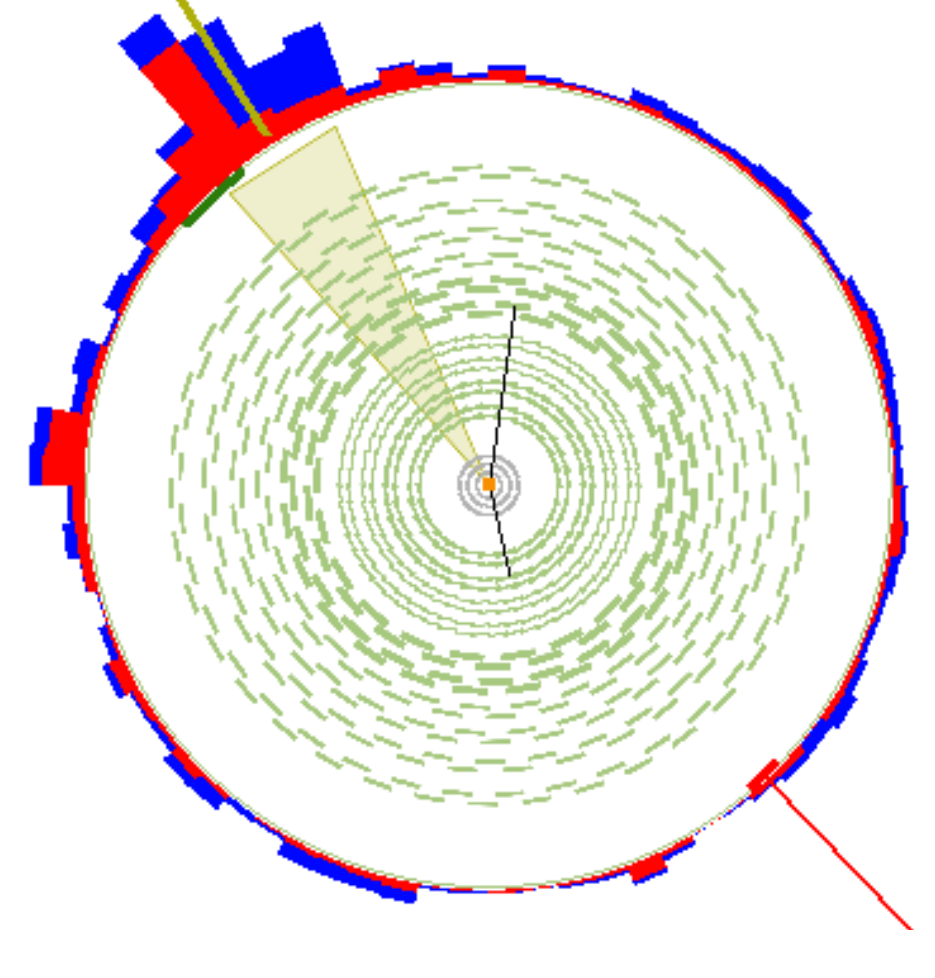
\includegraphics[width=0.31\textwidth]{figures/analysis/EventDisplay_scenario2_Zoomed.png}}
  \end{tabular}
  \caption{Visualisation of possible signatures of a chargino pair produced with a lifetime of $c\tau = 10\,\text{m}$ (left) and a lifetime of $c\tau = 0.5\,\text{m}$ (middle and right). 
           In the left picture, both charginos are reconstructed as muons, which can be seen in the energy deposition in the muon chambers (red boxes). 
           In the middle picture both charginos are only visible as tracks in the tracker (black lines), where both trajectories end inside the silicon tracker, showing the decay point point of the corresponding chargino. 
           The right picture is a zoom of the picture in the middle. Here only the cross-section of the tracker (green wavy lines) is displayed. The red arrow shows the missing transverse energy in the event.} 
  \label{fig:CharginoPaiEventDisplay}
\end{figure}
As mentioned before, this analysis targets a search for supersymmetry with charginos of lifetimes between $10\,\text{cm} \lesssim c\tau \lesssim  40\,\text{cm}$.
That means that the charginos decay rather early in the detector, even at the beginning of the tracker. 
The distinct challenges of such an analysis, shall be listed in the following passage.

First of all, in case R-parity (see Sec.~\ref{theorySUSY}) is conserved, one of the decay products of the chargino, which is the lightest neutralino \chiO is stable, thus travelling through the whole detector only weakly intereacting.
Therefore it is not detectable. 
The other chargino decay product, e.g. a pion, can be hardly reconstructed, mainly because it does not origin from the primary vertex (if the chargino reaches the detector before its decay), 
but secondarily because it is very low in momentum because of the mass-degeneracy between \chipm and \chiO.
The momentum of the decay product is of course highly dependent on the actual mass gap between the neutralino and the chargino.
A typical \pt distribution of a pion originating from a chargino decay can be found in Fig.~\ref{fig:KinkedTrack} for a mass gap between \chipm and \chiO of 150\,\mev.
\begin{figure}[!t]
  \centering 
  \begin{tabular}{c}
    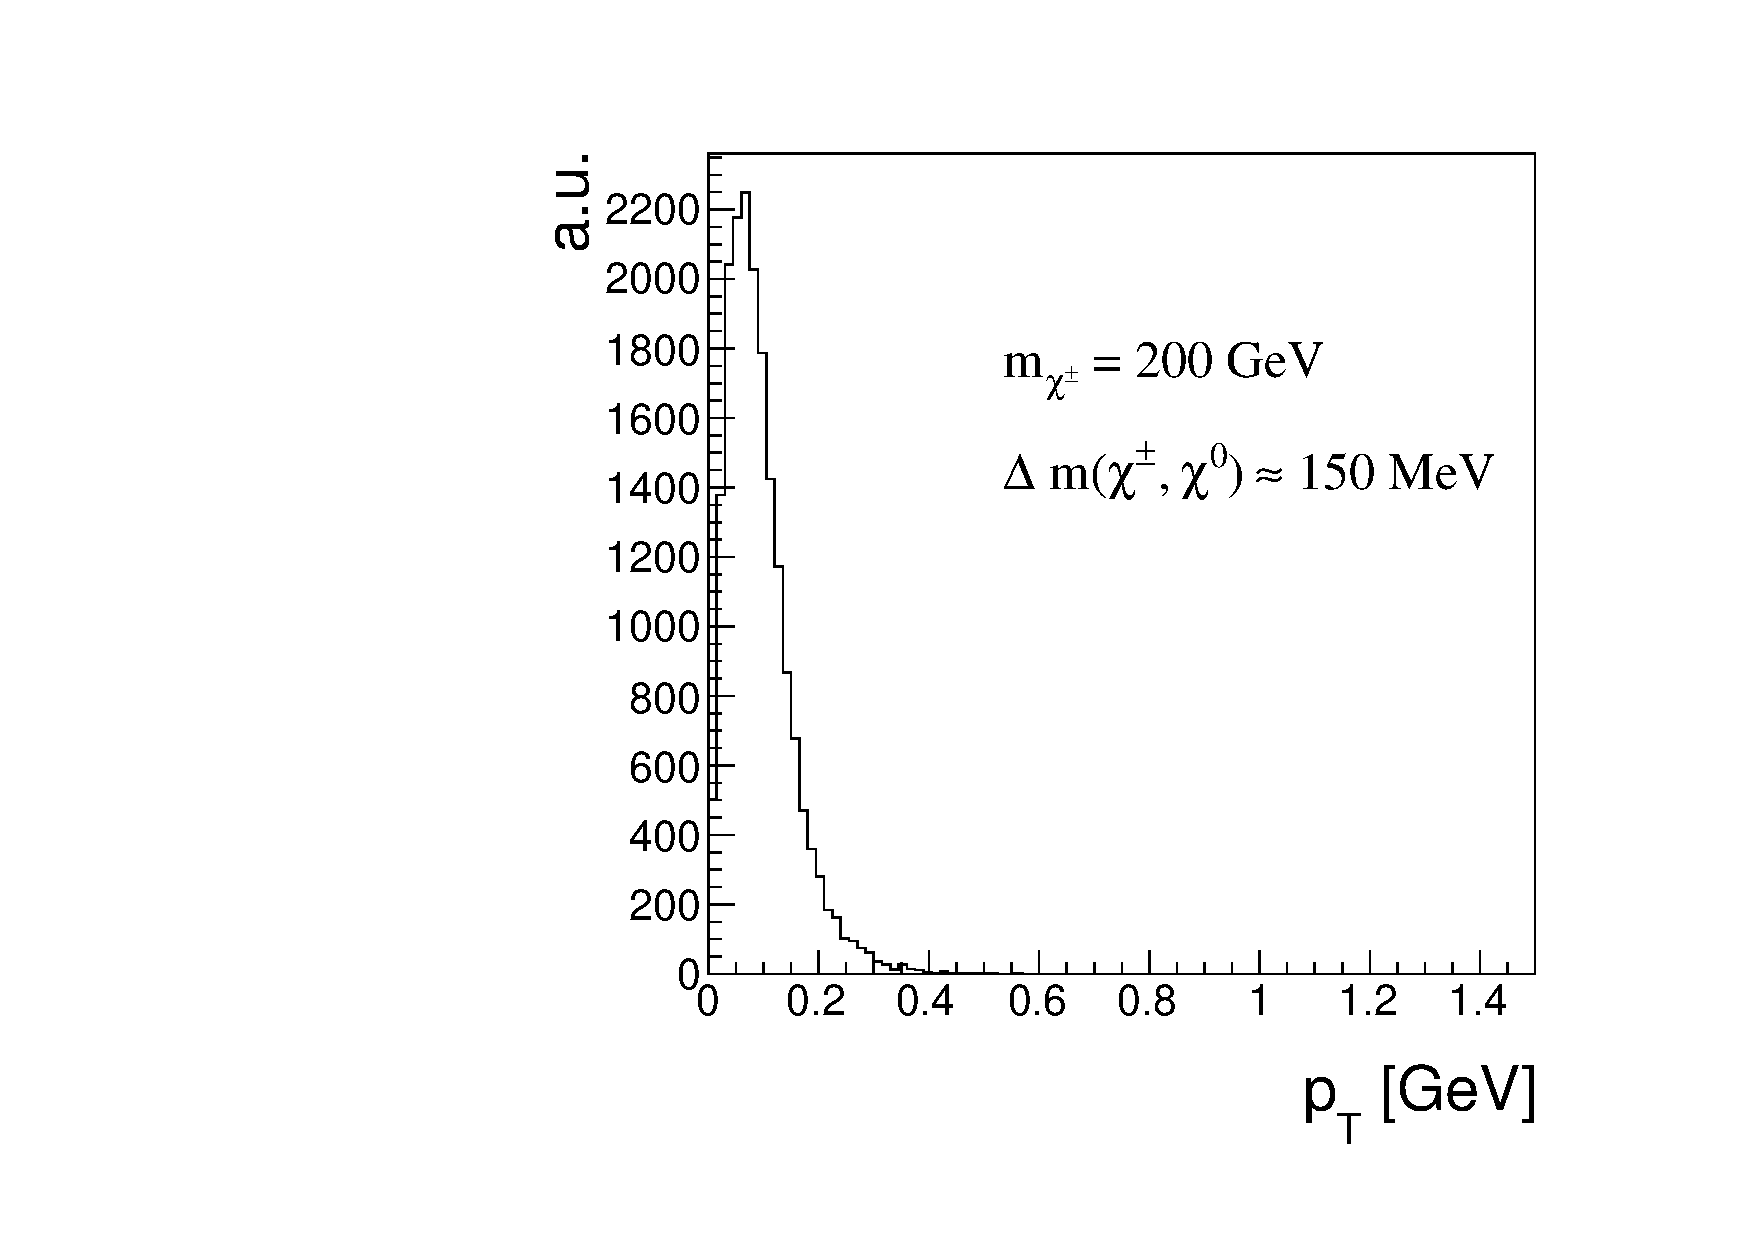
\includegraphics[width=0.6\textwidth]{figures/analysis/ptOfPions.pdf}
  \end{tabular}
  \caption{Transverse momentum distribution of pions coming from chargino decay into a neutralino with a mass gap of 150\mev.}
  \label{fig:ptOfPions}
\end{figure} 
The \pt distribution peaks at \mbox{$\sim$ 100\,\mev} and ends at \mbox{\pt $\sim 400\,$\mev}.
When the transverse momentum of a particle is very low, the particle trajectory is much more bended compared to a particle with higher \pt (see Fig.~\ref{fig:KinkedTrack} for illustration), 
thus making the detection of such a particle very challinging.
\begin{figure}[!bt]
  \centering 
  \begin{tabular}{c}
    \frame{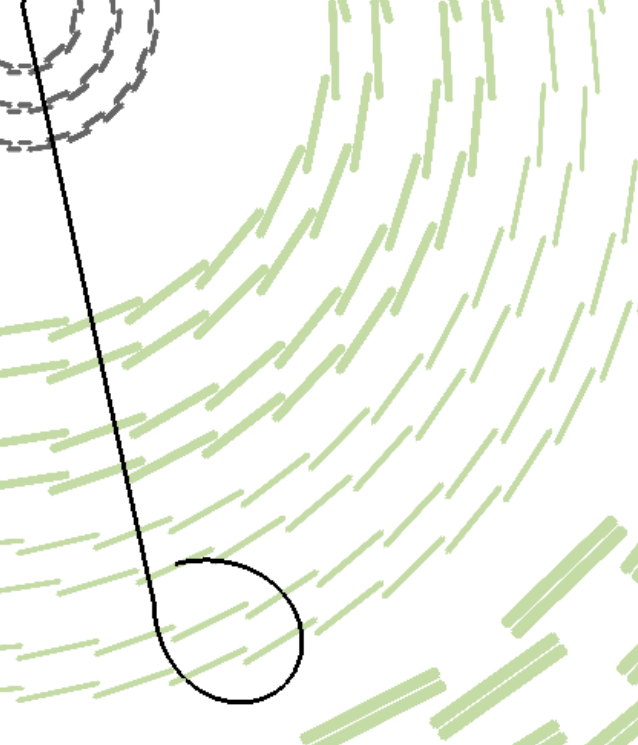
\includegraphics[width=0.3\textwidth]{figures/analysis/KinkedTrackZoom.png}}
  \end{tabular}
  \caption{Cross-sectional view of the tracker (different tracker layers are illustrated with wavy green lines) and a simulated chargino track (black line) decays to a pion (bended black line).}
  \label{fig:KinkedTrack}
\end{figure} 
Because of the stronger bending, the track reconstruction efficiency decreases for particles with a transverse momentum below 1\,\gev rapidely, ending at around 40\% for isolated pions with a \pt of 100\mev (see \cite{bib:CMS:tracking_8TeV}).

Taking the hard or even impossible detection of the decay products of the chargino, this lead to the fact, that besides the (short) track of the chargino, nothing can be seen in the detector.
Unfortunately, there is no dedicated track trigger at CMS, which makes a specific detection of those events with the help of the chargino track impossible.
To be able to search for these models, one therefore need to take advantage of higher order contributions to the feynman diagrams shown in the previous sections (Figs.~\ref{fig:FeynmanDiagramProductionCharginoPair},\ref{fig:FeynmanDiagramProductionCharginoNeutralino}), resulting in initial state radiation (ISR).
When the initial quarks radiate a high \pt gluon, the resulting jet can be detected and can offer a possibility to search for isolated tracks in the tracker.
The non-detection of the chargino's decay products plus a high \pt ISR jet lead additionally to missing transverse energy (MET) in the event. 
Exploiding these two circumstances, it is possible to detect chargino-pair or chargino-neutralino events with the help of Jet+MET triggers.\\

To select possible charginos in an event, additional requirements for isolated, high \pt tracks are needed.
Those tracks can be eventually disappearing, which means that the track does not cross the full pixel and strip detector.
This can happen, when the chargino decays inside the tracker.
For very low lifetimes, the tracks can be very short and can have only a few hits in the detector. 
To define a helical path five parameters are needed, therefore a minimum of three hits are required to be able to reconstruct a particle's trajetcory (see \cite{bib:CMS:tracking_8TeV}).
In this analysis, the massiveness of the charginos shall be exploited, on the one hand by selecting only high \pt tracks, but on the other hand by requiering a high energy deposition per path length (\dedx).
The energy deposition depends quadratically on the particle's mass for low velocities ($0.2<\beta\gamma<0.9$).
\begin{equation}
\langle\frac{dE}{dx}\rangle = K \frac{m^2}{p^2} +C
\end{equation}

thus constitute a very nice discriminating variable for massive particles. 
A specific challenge for this analysis is the combinitation of searching for short tracks and utilising the energy deposition of the chargino.
Unfortunately, the pixel tracker during Run I underwent only a calibration procedure at the very beginning of the start of data taking in 2011.
Because of various readjustments during the year 2012, this introduced a huge non-calibration over time. 
In case we want to look at the \dedx of the tracks, there is therefore the need to recalibrate the pixel detector in order to be able to use its energy information in this analysis.

%\begin{itemize}
%\item No detection of low momentum fermions possible (fermion pt plot?), no detection of the decay products
%\item Concentration on intermediate lifetime $\rightarrow$ only a (short) chargino track can be seen.
%\item Show event displays and sketch for pion decyay!
%\item Detection via ISR 
%\item Event selection by ISR jet and MET
%\item Detection of track (possibly short and disappearing and highly ionizing, not reconstructed as muon)
%\item Short and highly ionizing track $\rightarrow$ inclusion of pixel tracker information 
%\end{itemize}

\subsection{Comparison to existing searches}
As already mentioned before, there were several analyses at CMS, which are sensitive to intermediate lifetime charginos. 
Most notably, the search for long lived-charged particles \cite{bib:CMS:HSCP_8TeV} and the search for disappering tracks \cite{bib:CMS:DT_8TeV}.
An improvement in sensitivity to shorter lifetimes compared to these analysis shall be achieved by including also very short tracks in this analysis.
In \cite{bib:CMS:HSCP_8TeV}, a minimum number of eight hits, whereas in \cite{bib:CMS:DT_8TeV} a minimum of seven hits are required. 
This can be very unefficient for shorter lifetimes, where most of the charginos decay already after the pixel tracker ($\sim 10\,\text{cm}$).
Additionally, the search for disappearing tracks does not make use of the high energy deposition of heavy particles. 
On the other hand is this variable used in the search for long-lived particles, where the sensitiviy decreases much quicker for shorter lifetimes (see Fig~\ref{fig:pMSSMplot}).
In \cite{bib:CMS:DT_8TeV}, there is a muon-veto exploited to supress SM background coming from processes resulting in one or two muons. 
Additionnally, it requires missing outer hits in the tracker (disappearing track), which makes this analysis especially sensitive to a shorter tracks.
In the preseneted analaysis, the stron selection on the number of hits in the tracker shall be lowered and the variable \dedx shall be included to increase sensitiviy.
Also, a muon-veto is applied to make the selection expecially sensitive to very short lifetimes.
\textcolor{red}{MAYBE} show here already a plot with the number of valid hits distribution to emphasize the importance of lossening the number of hits cut!
%%%%%%%%%%%%%%%%%%%%%%%%%%%%%%%%%%%%%%%%%%%%%%%%%%%%%%%%%%%%%%%%%%%%%%%%%%%%%%%%%%%%%%%%%%%%%%%%%%%%%%%%%%%%%%%%%%%%%%%%%%%%%%%%%%%%%%%%%%%%%%%%%%%%%%%%%%%%%%%%%%%%%%%%%%%%%%%%%%%%
%%%%%%%%%%%%%%%%%%%%%%%%%%%%%%%%%%%%%%%%%%%%%%%%%%%%%%%%%%%%%%%%%%%%%%%%%%%%%%%%%%%%%%%%%%%%%%%%%%%%%%%%%%%%%%%%%%%%%%%%%%%%%%%%%%%%%%%%%%%%%%%%%%%%%%%%%%%%%%%%%%%%%%%%%%%%%%%%%%%%
\section{Improved dE/dx measurement of short tracks}
\label{sec:DeDxMeasurement}
It was already pointed out, that the inclusion of the pixel energy measurements can increase the sensitivity when searching especially for short tracks.
While the silicon strip detetcor has already been calibrated as part of the search for long-lived charged particles \cite{bib:CMS:HSCP_8TeV}, there was never an offline calibration done for the pixel silicon tracker.
To increase the discrimination power of \dedx, such an calibration procedure was therefore conducted within this PHD thesis.
 
\subsection{Measuring dE/dx}
The mean energy loss per path length of particles travelling through a layer of material can be described with the Bethe-Bloch formula \cite{bib:Bethe_1930,bib:Bloch_1933}:
\begin{equation}
\langle \frac{dE}{dx} \rangle = kz^2\frac{Z}{A}\frac{1}{\beta^2} [ \frac{1}{2} \ln{\frac{2m_e c^2 \beta^2 \gamma^2 T_{\text{max}}}{I^2}} - \beta^2 - \frac{\delta( \beta \gamma )}{2} ].
\end{equation}
It is valid, where the main energy loss originates from ionization effects which is in a region between $0.1\lesssim\beta\gamma\lesssim 1000$.
It is a function of the atomic number ($Z$) and the atomic mass of the absorber ($A$). 
The mean excitation energy ($I$) for silicon is 173$\pm$3\,eV \cite{?}. 
$T_{\text{max}}$ stands for the maximum energy transfer in a single collision.
The relevant particle's properties are the velocity ($\beta$), the lorentz factor ($\gamma$) and the charge (z) of the incident particle.
The density correction $\delta( \beta \gamma )$ reduces the mean energy loss at high energies because of polarization effects of the material.

Even if widely used, the Bethe-Bloch formula is ill-defined because of the use of the mean energy loss per path length.
The problem arises when looking at the fluctuations of a particle's energy deposition.
In case particles cross material layers of moderate sickness, the probability density function of the deposited energy can be described by a Landau function \cite{bib:Landau_1944}. 
The Landau distribution is a highly asymmetric distribution with a long tail torwards the right end (see Fig.~\ref{fig:landau}).
Theoretically it extends to infinite energies, however in nature the maximal deposited energy is of course limited by the particle's full energy.
\begin{figure}[!t]
  \centering 
  \begin{tabular}{c}
  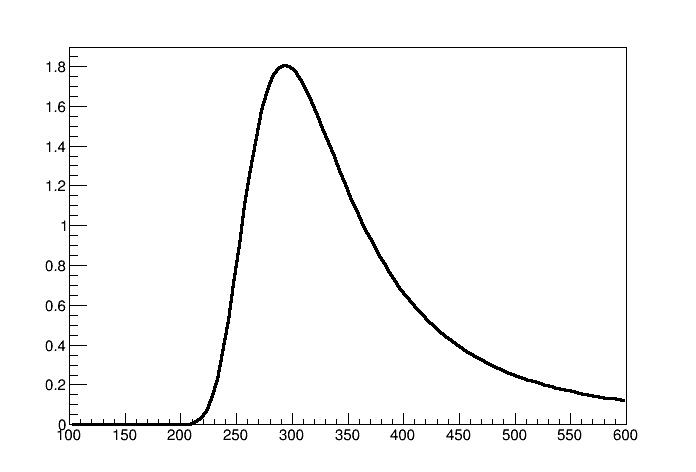
\includegraphics[width=0.5\textwidth]{figures/analysis/landau.png}
  \end{tabular}
  \caption{Illustration of a Landau function. Parameters were arbitrarily chosen for this figure.} 
  \label{fig:landau}
\end{figure}
The mean and the variance of a landau distribution are not defined. 
This is again different for a (limited) measurment, as there it is always possible to calucalute a mean.
Still, this leads to the fact that the definition of the mean energy loss per path length is a problematic and unstable concept.
A much better observable is the most probably value (MPV) being the maximum of the landau function, which is much more stable compared to the mean. 
The most probable energy loss of a charged particle is defined by the Landau-Vavilov-Bichsel equation:
\begin{equation}
\Delta_p = \xi \left[ \ln \frac{2mc^2\beta^2\gamma^2}{I}  + \ln\frac{\xi}{I} + j - \beta^2 - \delta(\beta\gamma)  \right],
\end{equation}
where $\xi=(K/Z)\langle Z/A \rangle (x/\beta^2)$. 
The thickness of the absorber $x$ appears explicitly in the Landau-Vavilov-Bichsel equation making the most probable energy loss per path \mbox{length $\frac{\Delta_p}{dx}$} logarithmically dependent on $x$.
A comparison between the Bethe mean energy loss $\langle \frac{dE}{dx} \rangle$ and the most probable energy loss $\frac{\Delta_p}{dx}$ are shown in Fig.~\ref{fig:dEdx_Bethe_Landau}.
\begin{figure}[!bt]
  \centering 
  \begin{tabular}{c}
  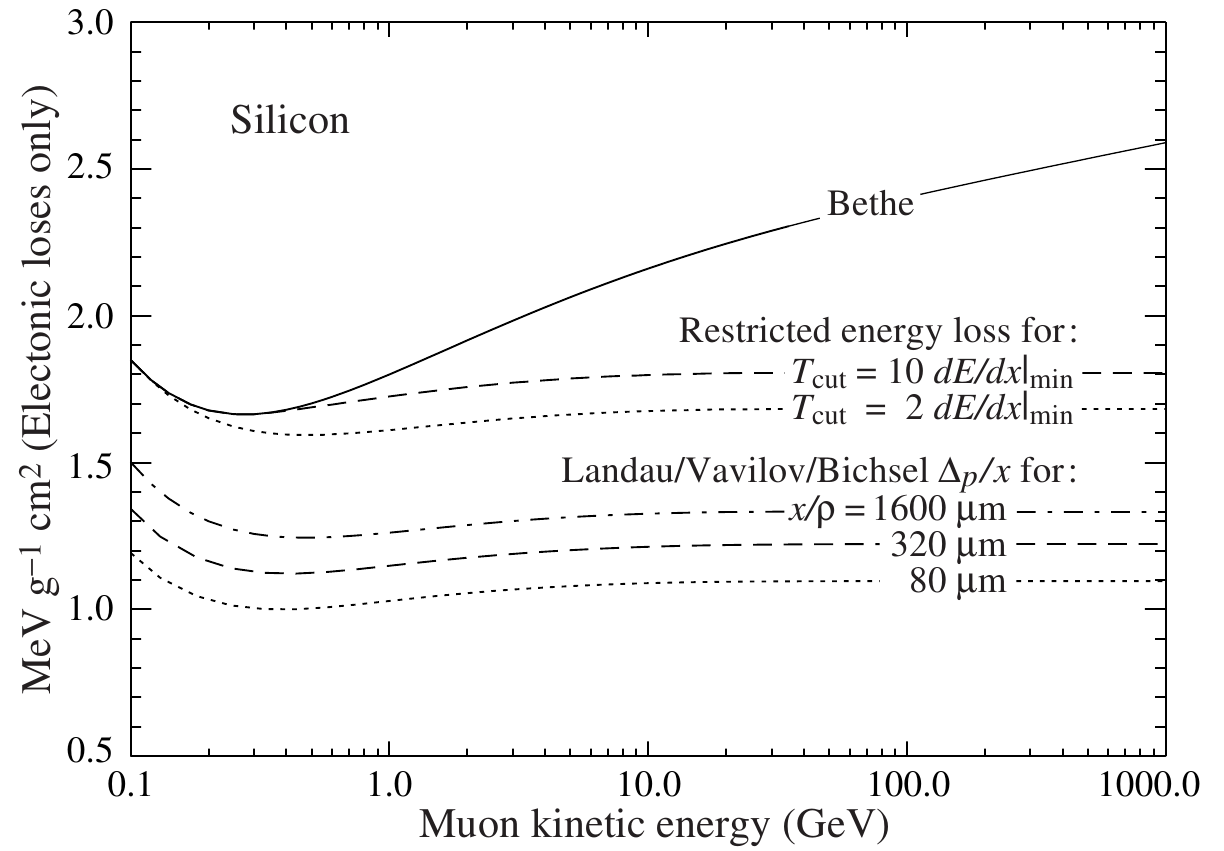
\includegraphics[width=0.5\textwidth]{figures/analysis/dEdx_Bethe_Landau.png}
  \end{tabular}
  \caption{Comparison between the Bethe mean energy loss with and without restricted energy loss and the most probable energy loss described by the Landau-Vavilov-Bichsel function for different sizes of thickness. 
           Taken from \cite{bib:PDG_2014}.} 
  \label{fig:dEdx_Bethe_Landau}
\end{figure}
\\

SM particles as pions and muons are minimal ionising in silicon for $\beta\gamma \sim 4$, dependent on the thickness of the material (see Fig.~\ref{fig:dEdx_Landau_Silicon} ). 
For higher momenta the deposited energies increase again reaching a plateau at around $\beta\gamma\sim100$. 
However, new heavy charged particles would mainly be unrelativistic because of their high mass and would therefore deposit much higher energies in the detector.
This makes the energy deposition per path length to a very well discriminating variable.
\begin{figure}[!bt]
  \centering 
  \begin{tabular}{c}
  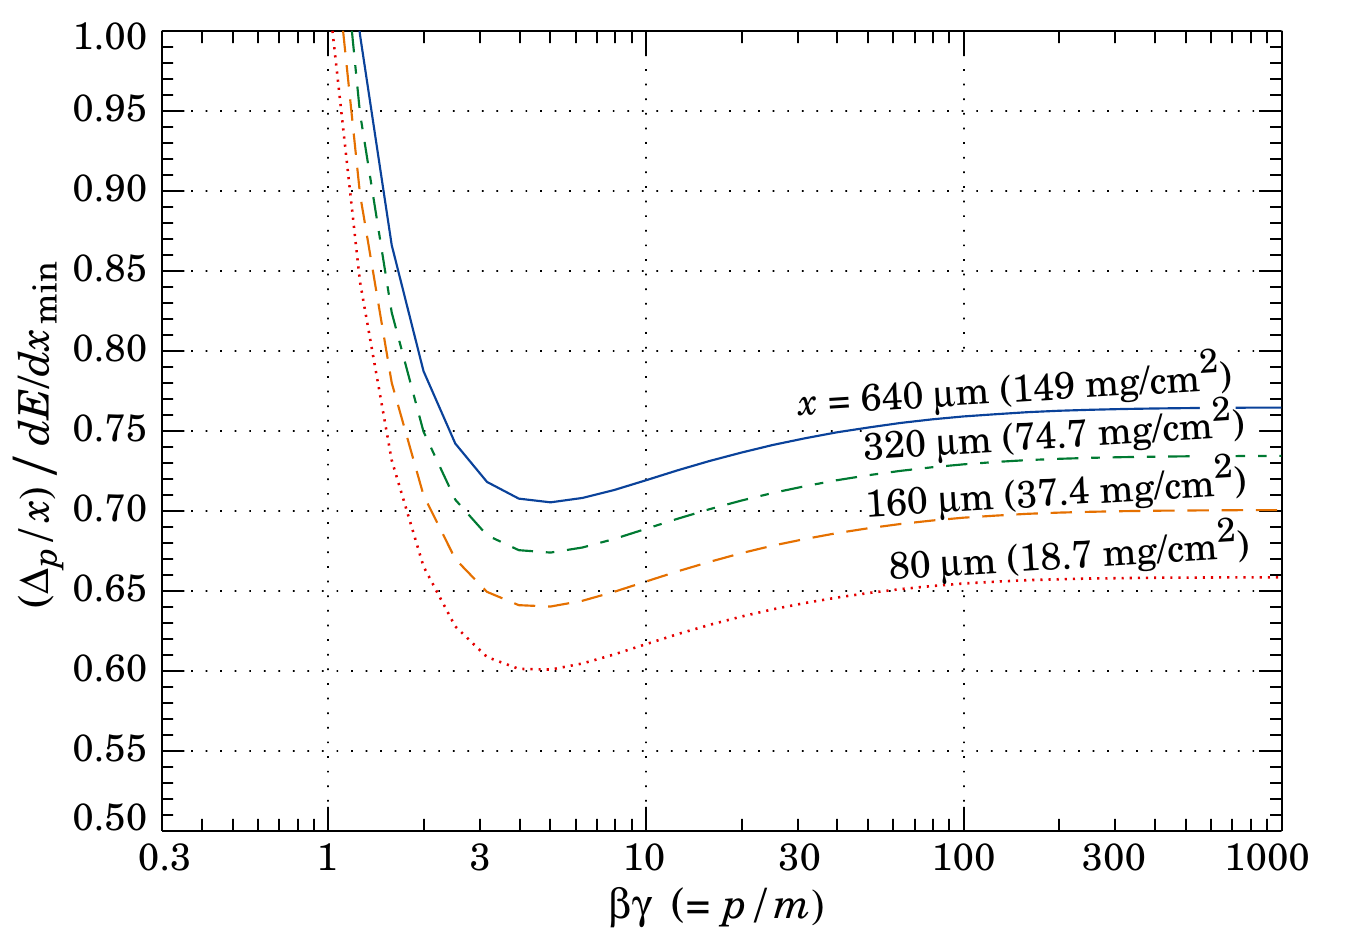
\includegraphics[width=0.5\textwidth]{figures/analysis/dEdx_Landau_Silicon.png}
  \end{tabular}
  \caption{Most probable energy loss in silicon, scaled to the mean loss of a minimal ionizing particle (388 eV/$\mu$m). Taken from \cite{bib:PDG_2014}.} 
  \label{fig:dEdx_Landau_Silicon}
\end{figure}
Thus, the energy loss per path length can be used to discriminate between SM particles and new heavy charged particles, which are usually unrelativistic because of their high mass.

%\begin{itemize}
%\item The variable dE/dx: General introdution
%\item Bethe-Bloch (difficult concept because of undefined mean of the Landau function)
%\item Landau distribution (no mean)
%\item Most probable energy loss landau vavilov function (show comparison plot Landau, Bethe)
%\item Minimal ionising particles (pt cut) (how dedx for pions CMS 2008)
%\end{itemize}

\subsection{Gain calibration of the silicon pixel tracker}

During Run I in 2012, the pixel silicon detector was continously subjected to an energy calibration, which is called gain calibration.
Every pixel was calibrated to the same response, such that the whole pixel tracker should be well inter-calibrated.
Unfortunately, due to imperfect constancy of the reference signal, the approximation of the atan() response with a linear function, and radiation and temperature induces changes, the energy calibration is not adequate to use the emasured energy deposition without further calibration.
This imperfection of the gain calibration can be seen in Fig.~\ref{fig:dEdx_beforeCalibration}, where the harmonic-2 estimator summed over all tracks  (see \cite{} for a detailed explanation) over time is shown.
Four different steps can be spotted. The first and the third correspond to a change  in the settings of the tracker, the second and fourth is, where a gain calibration was applied.
Unfortunately, although a gain calibration was applied (even with delay), it could not bring the average dE/dx to the same level before the change in the setting occured.
The size of the difference in the dE/dx measurement over time being around 10\% is too large to use the dE/dx out of the box.

\begin{figure}[!bt]
  \centering 
  \begin{tabular}{c}
  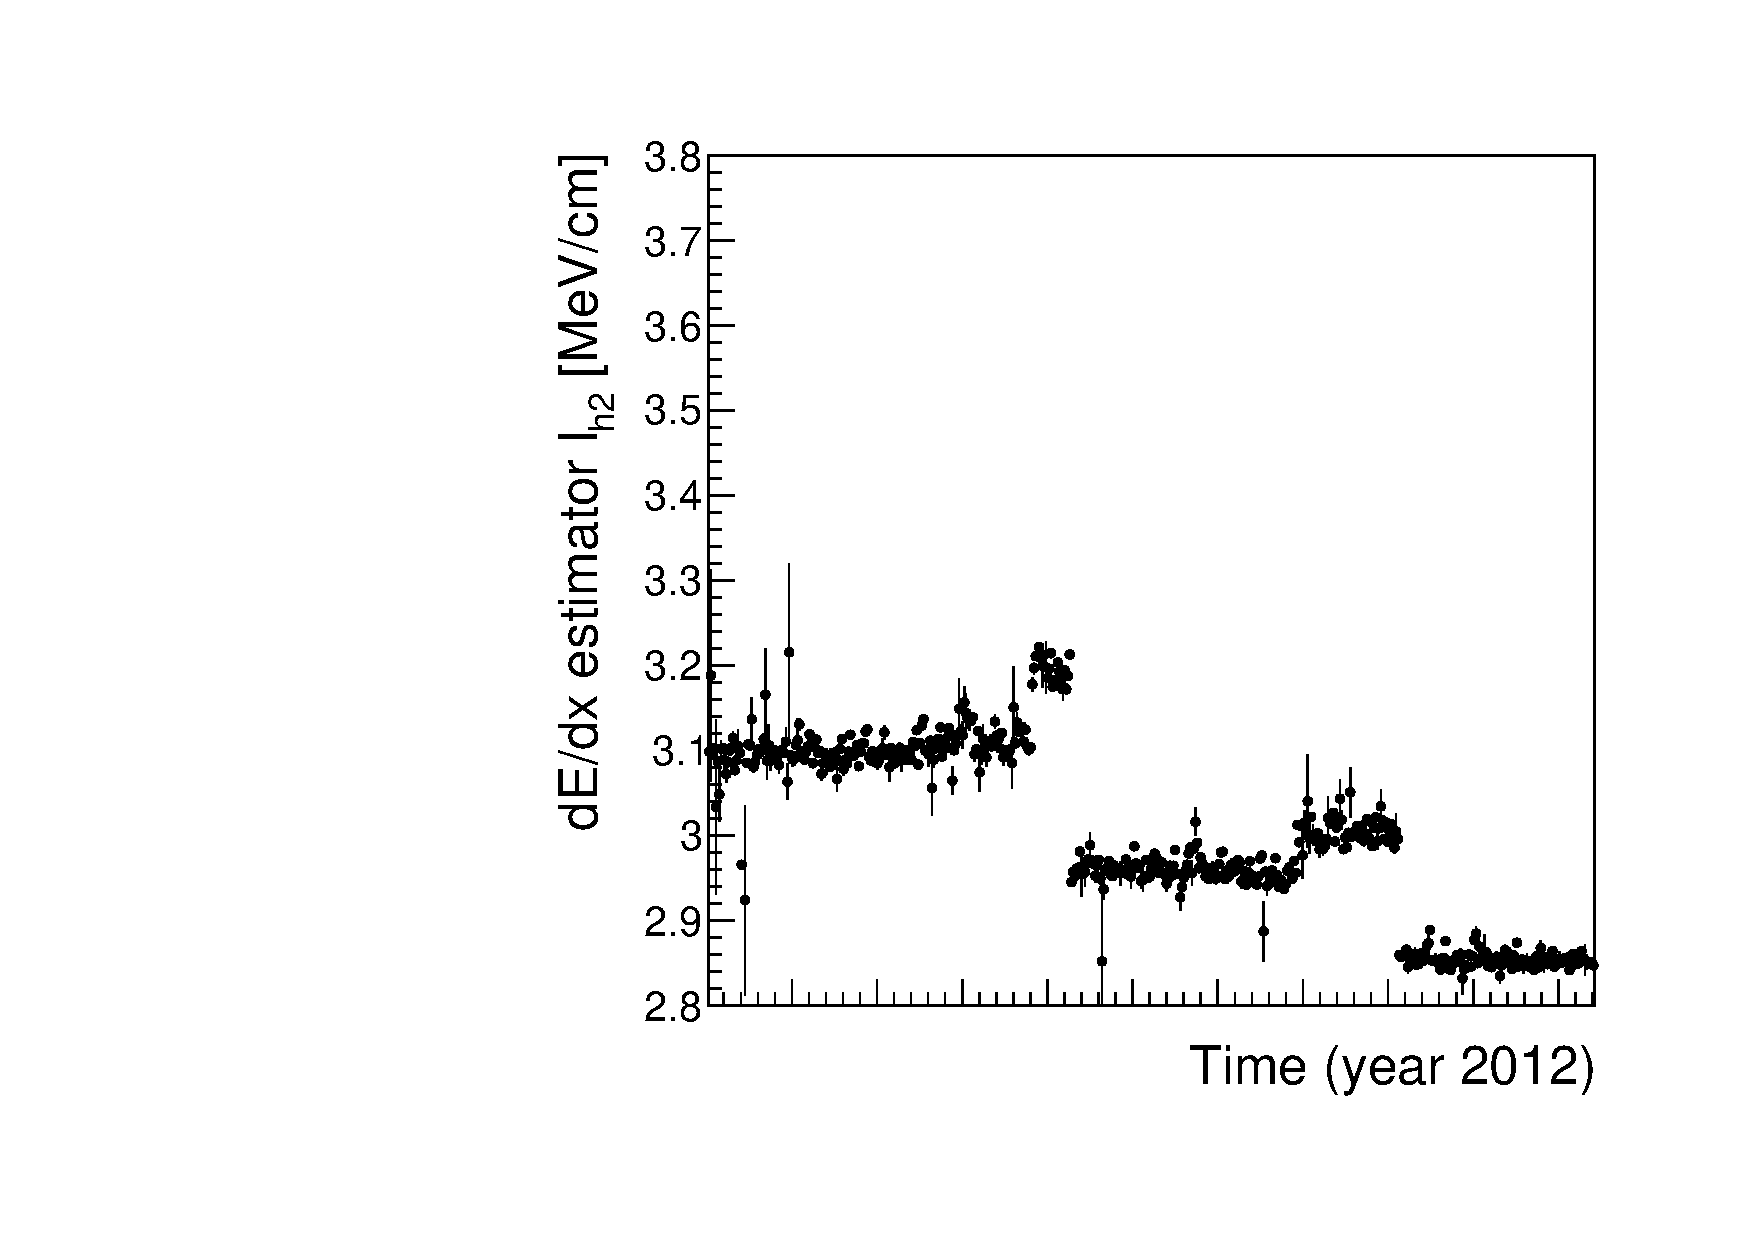
\includegraphics[width=0.5\textwidth]{figures/analysis/StabilityPlot_Pixel_beforeCalibration_withoutStepFits_NEW.pdf}
  \end{tabular}
  \caption{Sum of all track's dE/dx (harmonic-2 estimator) over the full year 2012. Every data point correspond to one run.} 
  \label{fig:dEdx_beforeCalibration}
\end{figure}

\begin{itemize}
\item What kind of calibrations are done with the silicon pixel and strip detectors?
\item Pixel detector has been calibrated once before ijecting it to CMS
\item dEdx not stable over time (show plot)
\item Describe the different levels of calibration (what is calibrated, pixels, what is not calibrated, ROC) (intercalibration of ROCs and a clibration vs. time)
\item How can the calibration been done (using MIPs, \pt cut, which samples are used - Min Bias samples)
\item Which validation procedure were conducted?
\item What are the results of the calibration
\end{itemize}

\subsection{Asymmetric Smirnov discriminator}

\subsection{Efficiency improvements}
%%%%%%%%%%%%%%%%%%%%%%%%%%%%%%%%%%%%%%%%%%%%%%%%%%%%%%%%%%%%%%%%%%%%%%%%%%%%%%%%%%%%%%%%%%%%%%%%%%%%%%%%%%%%%%%%%%%%%%%%%%%%%%%%%%%%%%%%%%%%%%%%%%%%%%%%%%%%%%%%%%%%%%%%%%%%%%%%%%%%
%%%%%%%%%%%%%%%%%%%%%%%%%%%%%%%%%%%%%%%%%%%%%%%%%%%%%%%%%%%%%%%%%%%%%%%%%%%%%%%%%%%%%%%%%%%%%%%%%%%%%%%%%%%%%%%%%%%%%%%%%%%%%%%%%%%%%%%%%%%%%%%%%%%%%%%%%%%%%%%%%%%%%%%%%%%%%%%%%%%%
\section{Simulated samples}
\label{sec:SimulatedSamples}
\subsection{SM samples}
\subsection{Signal samples}
%%%%%%%%%%%%%%%%%%%%%%%%%%%%%%%%%%%%%%%%%%%%%%%%%%%%%%%%%%%%%%%%%%%%%%%%%%%%%%%%%%%%%%%%%%%%%%%%%%%%%%%%%%%%%%%%%%%%%%%%%%%%%%%%%%%%%%%%%%%%%%%%%%%%%%%%%%%%%%%%%%%%%%%%%%%%%%%%%%%%
%%%%%%%%%%%%%%%%%%%%%%%%%%%%%%%%%%%%%%%%%%%%%%%%%%%%%%%%%%%%%%%%%%%%%%%%%%%%%%%%%%%%%%%%%%%%%%%%%%%%%%%%%%%%%%%%%%%%%%%%%%%%%%%%%%%%%%%%%%%%%%%%%%%%%%%%%%%%%%%%%%%%%%%%%%%%%%%%%%%%
\section{Event selection}
\label{sec:EventSelection}
\subsection{Datasets and triggers}
\begin{itemize}
\item Datasets and triggers used in the analysis
\item signal samples generated with Madgraph and pythia
\item They are decayed in Geant to only pions. Around ten different lifetimes were simulated
\item For other lifetimes: lifetime reweighting is done PLOT
\item For five diffenrent masses (100-500 GeV) 
\end{itemize}
\subsection{Preselection}
\begin{itemize}
\item Motivate different selection cuts
\item Reference DT search for most of them
\end{itemize}
\subsection{Main discriminating variables}
\begin{itemize}
\item dE/dx
\item pt
\item Show some MC signal bkg comparioson plots (only Wjets?)
\end{itemize}

%%%%%%%%%%%%%%%%%%%%%%%%%%%%%%%%%%%%%%%%%%%%%%%%%%%%%%%%%%%%%%%%%%%%%%%%%%%%%%%%%%%%%%%%%%%%%%%%%%%%%%%%%%%%%%%%%%%%%%%%%%%%%%%%%%%%%%%%%%%%%%%%%%%%%%%%%%%%%%%%%%%%%%%%%%%%%%%%%%%%
\section{Sources of backgrounds}
\label{sec:SourcesOfBackgrounds}
\begin{itemize}
\item Background consist of particles which make high energy deposits and are high pt
\item In general: Low background search
\end{itemize}
\subsection{Fake tracks}
\begin{itemize}
\item Definition of fake tracks
\item How can they fake the signal
\end{itemize}
\subsection{Muons}
\begin{itemize}
\item How can muons fake the signal
\end{itemize}
\subsection{Pions}
\begin{itemize}
\item How can pions fake the signal
\end{itemize}
\subsection{Electrons}
\begin{itemize}
\item How can electrons fake the signal
\end{itemize}
%%%%%%%%%%%%%%%%%%%%%%%%%%%%%%%%%%%%%%%%%%%%%%%%%%%%%%%%%%%%%%%%%%%%%%%%%%%%%%%%%%%%%%%%%%%%%%%%%%%%%%%%%%%%%%%%%%%%%%%%%%%%%%%%%%%%%%%%%%%%%%%%%%%%%%%%%%%%%%%%%%%%%%%%%%%%%%%%%%%%
%%%%%%%%%%%%%%%%%%%%%%%%%%%%%%%%%%%%%%%%%%%%%%%%%%%%%%%%%%%%%%%%%%%%%%%%%%%%%%%%%%%%%%%%%%%%%%%%%%%%%%%%%%%%%%%%%%%%%%%%%%%%%%%%%%%%%%%%%%%%%%%%%%%%%%%%%%%%%%%%%%%%%%%%%%%%%%%%%%%%
\section{Background estimation methods}
\label{sec:BackgroundEstimation}
\subsection{Fake background}
\subsection{Leptonic background}
\subsection{Systematic uncertainties}

%%%%%%%%%%%%%%%%%%%%%%%%%%%%%%%%%%%%%%%%%%%%%%%%%%%%%%%%%%%%%%%%%%%%%%%%%%%%%%%%%%%%%%%%%%%%%%%%%%%%%%%%%%%%%%%%%%%%%%%%%%%%%%%%%%%%%%%%%%%%%%%%%%%%%%%%%%%%%%%%%%%%%%%%%%%%%%%%%%%%
\section{Optimization of search sensitivity}
\label{sec:Optimization}
\begin{itemize}
\item Show plots
\item show table
\item Include NlostOuter here, too
\end{itemize}

%%%%%%%%%%%%%%%%%%%%%%%%%%%%%%%%%%%%%%%%%%%%%%%%%%%%%%%%%%%%%%%%%%%%%%%%%%%%%%%%%%%%%%%%%%%%%%%%%%%%%%%%%%%%%%%%%%%%%%%%%%%%%%%%%%%%%%%%%%%%%%%%%%%%%%%%%%%%%%%%%%%%%%%%%%%%%%%%%%%%
\section{Statistical Methods/ Limit setting}
\label{sec:LimitSetting}

%%%%%%%%%%%%%%%%%%%%%%%%%%%%%%%%%%%%%%%%%%%%%%%%%%%%%%%%%%%%%%%%%%%%%%%%%%%%%%%%%%%%%%%%%%%%%%%%%%%%%%%%%%%%%%%%%%%%%%%%%%%%%%%%%%%%%%%%%%%%%%%%%%%%%%%%%%%%%%%%%%%%%%%%%%%%%%%%%%%%
\section{Results}
\label{sec:Results}
\begin{itemize}
\item Data cutflowtable
\item Tables with results
\item One plot (4 bins: Prediction and data)
\end{itemize}

%%%%%%%%%%%%%%%%%%%%%%%%%%%%%%%%%%%%%%%%%%%%%%%%%%%%%%%%%%%%%%%%%%%%%%%%%%%%%%%%%%%%%%%%%%%%%%%%%%%%%%%%%%%%%%%%%%%%%%%%%%%%%%%%%%%%%%%%%%%%%%%%%%%%%%%%%%%%%%%%%%%%%%%%%%%%%%%%%%%%
\section{Interpretation}
\label{sec:Interpretation}
\subsection{Systematic uncertainties of simulated signal samples}
\subsection{Exclusion limits}
\begin{itemize}
\item 1-d limits
\item 2-d limits
\end{itemize}



% \chapter{Conclusions} \label{sec:Conclusion}
% wdhaodj



% \appendix
% \input{Appendix.tex}

\bibliographystyle{lucas_unsrt}
\bibliography{Thesis}


% \cleardoublepage
\thispagestyle{empty}
\chapter*{~}
% \input{Danksagung.tex}


\end{document}

% Improvements:
% - cleardoublepage


